%%%%%%%%%%%%%%%%%%%%%%%%%%%%%%%%%%%%%%%%%
% The Legrand Orange Book
% LaTeX Template
% Version 2.1.1 (14/2/16)
%
% This template has been downloaded from:
% http://www.LaTeXTemplates.com
%
% Original author:
% Mathias Legrand (legrand.mathias@gmail.com) with modifications by:
% Vel (vel@latextemplates.com)
%
% License:
% CC BY-NC-SA 3.0 (http://creativecommons.org/licenses/by-nc-sa/3.0/)
%
% Compiling this template:
% This template uses biber for its bibliography and makeindex for its index.
% When you first open the template, compile it from the command line with the 
% commands below to make sure your LaTeX distribution is configured correctly:
%
% 1) pdflatex main
% 2) makeindex main.idx -s StyleInd.ist
% 3) biber main
% 4) pdflatex main x 2
%
% After this, when you wish to update the bibliography/index use the appropriate
% command above and make sure to compile with pdflatex several times 
% afterwards to propagate your changes to the document.
%
% This template also uses a number of packages which may need to be
% updated to the newest versions for the template to compile. It is strongly
% recommended you update your LaTeX distribution if you have any
% compilation errors.
%
% Important note:
% Chapter heading images should have a 2:1 width:height ratio,
% e.g. 920px width and 460px height.
%
%%%%%%%%%%%%%%%%%%%%%%%%%%%%%%%%%%%%%%%%%

%----------------------------------------------------------------------------------------
%	PACKAGES AND OTHER DOCUMENT CONFIGURATIONS
%----------------------------------------------------------------------------------------

\documentclass[11pt,oneside,fleqn]{book} % Default font size and left-justified equations

%----------------------------------------------------------------------------------------

%%%%%%%%%%%%%%%%%%%%%%%%%%%%%%%%%%%%%%%%%
% The Legrand Orange Book
% Structural Definitions File
% Version 2.0 (9/2/15)
%
% Original author:
% Mathias Legrand (legrand.mathias@gmail.com) with modifications by:
% Vel (vel@latextemplates.com)
% 
% This file has been downloaded from:
% http://www.LaTeXTemplates.com
%
% License:
% CC BY-NC-SA 3.0 (http://creativecommons.org/licenses/by-nc-sa/3.0/)
%
%%%%%%%%%%%%%%%%%%%%%%%%%%%%%%%%%%%%%%%%%

%----------------------------------------------------------------------------------------
%	VARIOUS REQUIRED PACKAGES AND CONFIGURATIONS
%----------------------------------------------------------------------------------------

\usepackage[top=3cm,bottom=3cm,left=3cm,right=3cm,headsep=10pt,a4paper]{geometry} % Page margins

\usepackage{graphicx} % Required for including pictures
\graphicspath{{Pictures/}} % Specifies the directory where pictures are stored
\usepackage{overpic} 

\usepackage{lipsum} % Inserts dummy text

\usepackage{tikz} % Required for drawing custom shapes

\usepackage[english]{babel} % English language/hyphenation

\usepackage{enumitem} % Customize lists
\setlist{nolistsep} % Reduce spacing between bullet points and numbered lists

\usepackage{booktabs} % Required for nicer horizontal rules in tables

\usepackage{float} % I (Amelia) did this to arrange my figs, if it breaks something sorry you can remove it. lmk though

\usepackage{xcolor} % Required for specifying colors by name
\definecolor{ocre}{RGB}{200,0,0} % Define the orange color used for highlighting throughout the book
\definecolor{yel}{RGB}{200,200,0}
\definecolor{purble}{RGB}{0,0,220}
%----------------------------------------------------------------------------------------
%	FONTS
%----------------------------------------------------------------------------------------
%\usepackage[lining]{CormorantGaramond}
%\newcommand{\titlefont}{\fontfamily{CormorantGaramond-LF}\selectfont}

\usepackage{fetamont}
\newcommand{\titlefont}{\fontfamily{ffm}\selectfont}

\usepackage{shadowtext}
\shadowoffset{2pt}
\shadowcolor{red!100} 

\usepackage{avant} % Use the Avantgarde font for headings
%\usepackage{times} % Use the Times font for headings
%\usepackage{mathptmx} % Use the Adobe Times Roman as the default text font together with math symbols from the Sym­bol, Chancery and Com­puter Modern fonts
%\usepackage[sfdefault]{biolinum}
%\usepackage{concrete}
\usepackage{mathpazo}
%\usepackage{quattrocento}
%\newcommand{\titlefont}{\quattrocentofont}

\usepackage{subcaption}
\usepackage{microtype} % Slightly tweak font spacing for aesthetics
\usepackage[utf8]{inputenc} % Required for including letters with accents
\usepackage[T1]{fontenc} % Use 8-bit encoding that has 256 glyphs
\usepackage{scalefnt}
\usepackage{xcolor,colortbl}
\usepackage[rightcaption]{sidecap}

\usepackage{avant}

\newcommand{\vm}[1]{{\color{violet}{VM: #1}}}
%----------------------------------------------------------------------------------------
%	BIBLIOGRAPHY AND INDEX
%----------------------------------------------------------------------------------------

\usepackage{csquotes}
\usepackage[style=alphabetic,citestyle=numeric,sorting=nyt,sortcites=true,autopunct=true,autolang=hyphen,hyperref=true,abbreviate=false,backref=true,backend=biber,defernumbers=true]{biblatex}
\addbibresource{bibliography.bib} % BibTeX bibliography file
\defbibheading{bibempty}{}

\usepackage{calc} % For simpler calculation - used for spacing the index letter headings correctly
\usepackage{makeidx} % Required to make an index
\makeindex % Tells LaTeX to create the files required for indexing

%----------------------------------------------------------------------------------------
%	MAIN TABLE OF CONTENTS
%----------------------------------------------------------------------------------------

\usepackage{titletoc} % Required for manipulating the table of contents

\contentsmargin{0cm} % Removes the default margin

% Part text styling
\titlecontents{part}[0cm]
{\addvspace{20pt}\centering\large\bfseries}
{}
{}
{}

% Chapter text styling
\titlecontents{chapter}[1.25cm] % Indentation
{\addvspace{12pt}\large\sffamily\bfseries\hypersetup{linkcolor=ocre}} 
 % Spacing and font options for chapters
{\color{ocre!60}\contentslabel[\Large\thecontentslabel]{1.25cm}\color{ocre}} % Chapter number
{\color{ocre}}  
{\color{ocre!60}\normalsize\;\titlerule*[.5pc]{.}\;\thecontentspage} % Page number

% Section text styling
\titlecontents{section}[1.25cm] % Indentation
{\addvspace{3pt}\sffamily\bfseries} % Spacing and font options for sections
{\contentslabel[\thecontentslabel]{1.25cm}} % Section number
{}
{\hfill\color{black}\thecontentspage} % Page number
[]

% Subsection text styling
\titlecontents{subsection}[1.25cm] % Indentation
{\addvspace{1pt}\sffamily\small} % Spacing and font options for subsections
{\contentslabel[\thecontentslabel]{1.25cm}} % Subsection number
{}
{\ \titlerule*[.5pc]{.}\;\thecontentspage} % Page number
[]

% List of figures
\titlecontents{figure}[0em]
{\addvspace{-5pt}\sffamily}
{\thecontentslabel\hspace*{1em}}
{}
{\ \titlerule*[.5pc]{.}\;\thecontentspage}
[]

% List of tables
\titlecontents{table}[0em]
{\addvspace{-5pt}\sffamily}
{\thecontentslabel\hspace*{1em}}
{}
{\ \titlerule*[.5pc]{.}\;\thecontentspage}
[]

%----------------------------------------------------------------------------------------
%	MINI TABLE OF CONTENTS IN PART HEADS
%----------------------------------------------------------------------------------------

% Chapter text styling
\titlecontents{lchapter}[0em] % Indenting
{\addvspace{15pt}\large\sffamily\bfseries} % Spacing and font options for chapters
{\color{ocre}\contentslabel[\Large\thecontentslabel]{1.25cm}\color{ocre}} % Chapter number
{}  
{\color{ocre}\normalsize\sffamily\bfseries\;\titlerule*[.5pc]{.}\;\thecontentspage} % Page number

% Section text styling
\titlecontents{lsection}[0em] % Indenting
{\sffamily\small} % Spacing and font options for sections
{\contentslabel[\thecontentslabel]{1.25cm}} % Section number
{}
{}

% Subsection text styling
\titlecontents{lsubsection}[.5em] % Indentation
{\normalfont\footnotesize\sffamily} % Font settings
{}
{}
{}

%----------------------------------------------------------------------------------------
%	PAGE HEADERS
%----------------------------------------------------------------------------------------

\usepackage{fancyhdr} % Required for header and footer configuration

\pagestyle{fancy}
\renewcommand{\chaptermark}[1]{\markboth{\sffamily\normalsize\bfseries\chaptername\ \thechapter.\ #1}{}} % Chapter text font settings
\renewcommand{\sectionmark}[1]{\markright{\sffamily\normalsize\thesection\hspace{5pt}#1}{}} % Section text font settings
\fancyhf{} \fancyhead[LE,RO]{\sffamily\normalsize\thepage} % Font setting for the page number in the header
\fancyhead[LO]{\rightmark} % Print the nearest section name on the left side of odd pages
\fancyhead[RE]{\leftmark} % Print the current chapter name on the right side of even pages
\renewcommand{\headrulewidth}{0.5pt} % Width of the rule under the header
\addtolength{\headheight}{2.5pt} % Increase the spacing around the header slightly
\renewcommand{\footrulewidth}{0pt} % Removes the rule in the footer
\fancypagestyle{plain}{\fancyhead{}\renewcommand{\headrulewidth}{0pt}} % Style for when a plain pagestyle is specified

% Removes the header from odd empty pages at the end of chapters
\makeatletter
\renewcommand{\cleardoublepage}{
\clearpage\ifodd\c@page\else
\hbox{}
\vspace*{\fill}
\thispagestyle{empty}
\newpage
\fi}

%----------------------------------------------------------------------------------------
%	THEOREM STYLES
%----------------------------------------------------------------------------------------

\usepackage{amsmath,amsfonts,amssymb,amsthm} % For math equations, theorems, symbols, etc

\newcommand{\intoo}[2]{\mathopen{]}#1\,;#2\mathclose{[}}
\newcommand{\ud}{\mathop{\mathrm{{}d}}\mathopen{}}
\newcommand{\intff}[2]{\mathopen{[}#1\,;#2\mathclose{]}}
\newtheorem{notation}{Notation}[chapter]

% Boxed/framed environments
\newtheoremstyle{ocrenumbox}% % Theorem style name
{0pt}% Space above
{0pt}% Space below
{\normalfont}% % Body font
{}% Indent amount
{\small\bf\sffamily\color{ocre}}% % Theorem head font
{\;}% Punctuation after theorem head
{0.25em}% Space after theorem head
{\small\sffamily\color{ocre}\thmname{#1}\nobreakspace\thmnumber{\@ifnotempty{#1}{}\@upn{#2}}% Theorem text (e.g. Theorem 2.1)
\thmnote{\nobreakspace\the\thm@notefont\sffamily\bfseries\color{black}---\nobreakspace#3.}} % Optional theorem note
\renewcommand{\qedsymbol}{$\blacksquare$}% Optional qed square

\newtheoremstyle{blacknumex}% Theorem style name
{5pt}% Space above
{5pt}% Space below
{\normalfont}% Body font
{} % Indent amount
{\small\bf\sffamily}% Theorem head font
{\;}% Punctuation after theorem head
{0.25em}% Space after theorem head
{\small\sffamily{\tiny\ensuremath{\blacksquare}}\nobreakspace\thmname{#1}\nobreakspace\thmnumber{\@ifnotempty{#1}{}\@upn{#2}}% Theorem text (e.g. Theorem 2.1)
\thmnote{\nobreakspace\the\thm@notefont\sffamily\bfseries---\nobreakspace#3.}}% Optional theorem note

\newtheoremstyle{blacknumbox} % Theorem style name
{0pt}% Space above
{0pt}% Space below
{\normalfont}% Body font
{}% Indent amount
{\small\bf\sffamily}% Theorem head font
{\;}% Punctuation after theorem head
{0.25em}% Space after theorem head
{\small\sffamily\thmname{#1}\nobreakspace\thmnumber{\@ifnotempty{#1}{}\@upn{#2}}% Theorem text (e.g. Theorem 2.1)
\thmnote{\nobreakspace\the\thm@notefont\sffamily\bfseries---\nobreakspace#3.}}% Optional theorem note

% Non-boxed/non-framed environments
\newtheoremstyle{ocrenum}% % Theorem style name
{5pt}% Space above
{5pt}% Space below
{\normalfont}% % Body font
{}% Indent amount
{\small\bf\sffamily\color{ocre}}% % Theorem head font
{\;}% Punctuation after theorem head
{0.25em}% Space after theorem head
{\small\sffamily\color{ocre}\thmname{#1}\nobreakspace\thmnumber{\@ifnotempty{#1}{}\@upn{#2}}% Theorem text (e.g. Theorem 2.1)
\thmnote{\nobreakspace\the\thm@notefont\sffamily\bfseries\color{black}---\nobreakspace#3.}} % Optional theorem note
\renewcommand{\qedsymbol}{$\blacksquare$}% Optional qed square
\makeatother

% Defines the theorem text style for each type of theorem to one of the three styles above
\newcounter{dummy} 
\numberwithin{dummy}{section}
\theoremstyle{ocrenumbox}
\newtheorem{theoremeT}[dummy]{Theorem}
\newtheorem{problem}{Problem}[chapter]
\newtheorem{exerciseT}{Exercise}[chapter]
\theoremstyle{blacknumex}
\newtheorem{exampleT}{Example}[chapter]
\theoremstyle{blacknumbox}
\newtheorem{vocabulary}{Vocabulary}[chapter]
\newtheorem{definitionT}{Definition}[section]
\newtheorem{corollaryT}[dummy]{Corollary}
\theoremstyle{ocrenum}
\newtheorem{proposition}[dummy]{Proposition}

%----------------------------------------------------------------------------------------
%	DEFINITION OF COLORED BOXES
%----------------------------------------------------------------------------------------

\RequirePackage[framemethod=TikZ]{mdframed}% Required for creating the theorem, definition, exercise and corollary boxes

% Theorem box
\newmdenv[roundcorner=5pt,
skipabove=7pt,
skipbelow=7pt,
backgroundcolor=black!5,
linecolor=ocre,
innerleftmargin=5pt,
innerrightmargin=5pt,
innertopmargin=5pt,
leftmargin=0cm,
rightmargin=0cm,
innerbottommargin=5pt]{tBox}

% Exercise box	  
\newmdenv[skipabove=7pt,
skipbelow=7pt,
rightline=false,
leftline=true,
topline=false,
bottomline=false,
roundcorner=10pt,
backgroundcolor=ocre!10,
linecolor=ocre,
innerleftmargin=5pt,
innerrightmargin=5pt,
innertopmargin=5pt,
innerbottommargin=5pt,
leftmargin=0cm,
rightmargin=0cm,
linewidth=4pt]{eBox}	

% Definition box
\newmdenv[skipabove=7pt,
skipbelow=7pt,
rightline=false,
leftline=true,
topline=false,
bottomline=false,
linecolor=ocre,
roundcorner=10pt,
innerleftmargin=5pt,
innerrightmargin=5pt,
innertopmargin=0pt,
leftmargin=1cm,
rightmargin=0cm,
linewidth=4pt,
innerbottommargin=0pt]{dBox}	

% Corollary box
\newmdenv[skipabove=7pt,
skipbelow=7pt,
rightline=false,
leftline=true,
topline=false,
bottomline=false,
linecolor=gray,
backgroundcolor=black!5,
roundcorner=10pt,
innerleftmargin=5pt,
innerrightmargin=5pt,
innertopmargin=5pt,
leftmargin=0cm,
rightmargin=0cm,
linewidth=4pt,
innerbottommargin=5pt]{cBox}

\newmdenv[skipabove=7pt,
skipbelow=7pt,
rightline=false,
leftline=true,
topline=false,
bottomline=false,
linecolor=gray,
backgroundcolor=black!5,
roundcorner=10pt,
innerleftmargin=5pt,
innerrightmargin=5pt,
innertopmargin=5pt,
leftmargin=1cm,
rightmargin=0cm,
linewidth=4pt,
innerbottommargin=5pt]{vBox}

% Creates an environment for each type of theorem and assigns it a theorem text style from the "Theorem Styles" section above and a colored box from above
\newenvironment{theorem}{\begin{tBox}\begin{theoremeT}}{\end{theoremeT}\end{tBox}}
\newenvironment{exercise}{\begin{eBox}\begin{exerciseT}}{\hfill{\color{ocre}\tiny\ensuremath{\blacksquare}}\end{exerciseT}\end{eBox}}				  
\newenvironment{definition}{\begin{dBox}\begin{definitionT}}{\end{definitionT}\end{dBox}}	
\newenvironment{example}{\begin{exampleT}}{\hfill{\tiny\ensuremath{\blacksquare}}\end{exampleT}}		
\newenvironment{corollary}{\begin{cBox}\begin{corollaryT}}{\end{corollaryT}\end{cBox}}	

%----------------------------------------------------------------------------------------
%	REMARK ENVIRONMENT
%----------------------------------------------------------------------------------------

\newenvironment{remark}{\par\vspace{10pt}\small % Vertical white space above the remark and smaller font size
\begin{list}{}{
\leftmargin=35pt % Indentation on the left
\rightmargin=25pt}\item\ignorespaces % Indentation on the right
\makebox[-2.5pt]{\begin{tikzpicture}[overlay]
\node[draw=ocre!60,line width=1pt,circle,fill=ocre!25,font=\sffamily\bfseries,inner sep=2pt,outer sep=0pt] at (-15pt,0pt){\textcolor{ocre}{R}};\end{tikzpicture}} % Orange R in a circle
\advance\baselineskip -1pt}{\end{list}\vskip5pt} % Tighter line spacing and white space after remark

%----------------------------------------------------------------------------------------
%	SECTION NUMBERING IN THE MARGIN
%----------------------------------------------------------------------------------------

\makeatletter
\renewcommand{\@seccntformat}[1]{\llap{\textcolor{ocre}{\csname the#1\endcsname}\hspace{1em}}}                    
\renewcommand{\section}{\@startsection{section}{1}{\z@}
{-4ex \@plus -1ex \@minus -.4ex}
{1ex \@plus.2ex }
{\normalfont\large\sffamily\bfseries}}
\renewcommand{\subsection}{\@startsection {subsection}{2}{\z@}
{-3ex \@plus -0.1ex \@minus -.4ex}
{0.5ex \@plus.2ex }
{\normalfont\sffamily\bfseries}}
\renewcommand{\subsubsection}{\@startsection {subsubsection}{3}{\z@}
{-2ex \@plus -0.1ex \@minus -.2ex}
{.2ex \@plus.2ex }
{\normalfont\small\sffamily\bfseries}}                        
\renewcommand\paragraph{\@startsection{paragraph}{4}{\z@}
{-2ex \@plus-.2ex \@minus .2ex}
{.1ex}
{\normalfont\small\sffamily\bfseries}}

%----------------------------------------------------------------------------------------
%	PART HEADINGS
%----------------------------------------------------------------------------------------

% numbered part in the table of contents
\newcommand{\@mypartnumtocformat}[2]{%
\setlength\fboxsep{0pt}%
\noindent\colorbox{ocre!20}{\strut\parbox[c][.7cm]{\ecart}{\color{ocre!70}\Large\sffamily\bfseries\centering#1}}\hskip\esp\colorbox{ocre!40}{\strut\parbox[c][.7cm]{\linewidth-\ecart-\esp}{\Large\sffamily\centering#2}}}%
%%%%%%%%%%%%%%%%%%%%%%%%%%%%%%%%%%
% unnumbered part in the table of contents
\newcommand{\@myparttocformat}[1]{%
\setlength\fboxsep{0pt}%
\noindent\colorbox{ocre!40}{\strut\parbox[c][.7cm]{\linewidth}{\Large\sffamily\centering#1}}}%
%%%%%%%%%%%%%%%%%%%%%%%%%%%%%%%%%%
\newlength\esp
\setlength\esp{4pt}
\newlength\ecart
\setlength\ecart{1.2cm-\esp}
\newcommand{\thepartimage}{}%
\newcommand{\partimage}[1]{\renewcommand{\thepartimage}{#1}}%
\def\@part[#1]#2{%
\ifnum \c@secnumdepth >-2\relax%
\refstepcounter{part}%
\addcontentsline{toc}{part}{\texorpdfstring{\protect\@mypartnumtocformat{\thepart}{#1}}{\partname~\thepart\ ---\ #1}}
\else%
\addcontentsline{toc}{part}{\texorpdfstring{\protect\@myparttocformat{#1}}{#1}}%
\fi%
\startcontents%
\markboth{}{}%
{\thispagestyle{empty}%
\begin{tikzpicture}[remember picture,overlay]%
\node at (current page.north west){\begin{tikzpicture}[remember picture,overlay]%	
\fill[ocre!20](0cm,0cm) rectangle (\paperwidth,-\paperheight);
\node[anchor=north] at (4cm,-3.25cm){\color{ocre!40}\fontsize{220}{100}\sffamily\bfseries\@Roman\c@part}; 
\node[anchor=south east] at (\paperwidth-1cm,-\paperheight+1cm){\parbox[t][][t]{8.5cm}{
\printcontents{l}{0}{\setcounter{tocdepth}{1}}%
}};
\node[anchor=north east] at (\paperwidth-1.5cm,-3.25cm){\parbox[t][][t]{15cm}{\strut\raggedleft\color{white}\fontsize{30}{30}\sffamily\bfseries#2}};
\end{tikzpicture}};
\end{tikzpicture}}%
\@endpart}
\def\@spart#1{%
\startcontents%
\phantomsection
{\thispagestyle{empty}%
\begin{tikzpicture}[remember picture,overlay]%
\node at (current page.north west){\begin{tikzpicture}[remember picture,overlay]%	
\fill[ocre!20](0cm,0cm) rectangle (\paperwidth,-\paperheight);
\node[anchor=north east] at (\paperwidth-1.5cm,-3.25cm){\parbox[t][][t]{15cm}{\strut\raggedleft\color{white}\fontsize{30}{30}\sffamily\bfseries#1}};
\end{tikzpicture}};
\end{tikzpicture}}
\addcontentsline{toc}{part}{\texorpdfstring{%
\setlength\fboxsep{0pt}%
\noindent\protect\colorbox{ocre!40}{\strut\protect\parbox[c][.7cm]{\linewidth}{\Large\sffamily\protect\centering #1\quad\mbox{}}}}{#1}}%
\@endpart}
\def\@endpart{\vfil\newpage
\if@twoside
\if@openright
\null
\thispagestyle{empty}%
\newpage
\fi
\fi
\if@tempswa
\twocolumn
\fi}

%----------------------------------------------------------------------------------------
%	CHAPTER HEADINGS
%----------------------------------------------------------------------------------------

% A switch to conditionally include a picture, implemented by  Christian Hupfer
\newif\ifusechapterimage
\usechapterimagetrue
\newcommand{\thechapterimage}{}%
\newcommand{\chapterimage}[1]{\ifusechapterimage\renewcommand{\thechapterimage}{#1}\fi}%
\newcommand{\thechapterimagecaption}{}%
\newcommand{\chapterimagecaption}[1]{\renewcommand{\thechapterimagecaption}{#1}}%
\def\@makechapterhead#1{%
{\parindent \z@ \raggedright \normalfont
\ifnum \c@secnumdepth >\m@ne
\if@mainmatter
\begin{tikzpicture}[remember picture,overlay]
\node at (current page.north west)
{\begin{tikzpicture}[remember picture,overlay]
\node[anchor=north west,inner sep=0pt] at (0,0) {\ifusechapterimage\includegraphics[width=\paperwidth]{\thechapterimage}\fi};
\draw[anchor=west] (\Gm@lmargin,-9cm) node [line width=2pt,rounded corners=15pt,draw=ocre,fill=white,fill opacity=0.5,inner sep=15pt]{\strut\makebox[22cm]{}};
\draw[anchor=west] (\Gm@lmargin+.3cm,-9cm) node {\huge\sffamily\bfseries\color{black}\thechapter. #1\strut};
\ifx\thechapterimagecaption\empty\else
  \node[anchor=north east, inner sep=4pt,
        fill=black, fill opacity=0.4, text opacity=1,
        rounded corners=2pt] at (\paperwidth -0.2cm, -0.3cm)
    {\small\sffamily\color{white}\thechapterimagecaption};
\fi
\end{tikzpicture}};
\end{tikzpicture}
\else
\begin{tikzpicture}[remember picture,overlay]
\node at (current page.north west)
{\begin{tikzpicture}[remember picture,overlay]
\node[anchor=north west,inner sep=0pt] at (0,0) {\ifusechapterimage\includegraphics[width=\paperwidth]{\thechapterimage}\fi};
\draw[anchor=west] (\Gm@lmargin,-9cm) node [line width=2pt,rounded corners=15pt,draw=ocre,fill=white,fill opacity=0.5,inner sep=15pt]{\strut\makebox[22cm]{}};
\draw[anchor=west] (\Gm@lmargin+.3cm,-9cm) node {\huge\sffamily\bfseries\color{black}#1\strut};
\ifx\thechapterimagecaption\empty\else
  \node[anchor=north east, inner sep=4pt,
        fill=black, fill opacity=0.4, text opacity=1,
        rounded corners=2pt] at (\paperwidth -0.2cm, -0.3cm)
    {\small\sffamily\color{white}\thechapterimagecaption};
\fi
\end{tikzpicture}};
\end{tikzpicture}
\fi\fi\par\vspace*{270\p@}}}


%-------------------------------------------

\def\@makeschapterhead#1{%
\begin{tikzpicture}[remember picture,overlay]
\node at (current page.north west)
{\begin{tikzpicture}[remember picture,overlay]
\node[anchor=north west,inner sep=0pt] at (0,0) {\ifusechapterimage\includegraphics[width=\paperwidth]{\thechapterimage}\fi};
\draw[anchor=west] (\Gm@lmargin,-9cm) node [line width=2pt,rounded corners=15pt,draw=ocre,fill=white,fill opacity=0.5,inner sep=15pt]{\strut\makebox[22cm]{}};
\draw[anchor=west] (\Gm@lmargin+.3cm,-9cm) node {\huge\sffamily\bfseries\color{black}#1\strut};
\ifx\thechapterimagecaption\empty\else
  \node[anchor=north east, inner sep=4pt,
        fill=black, fill opacity=0.4, text opacity=1,
        rounded corners=2pt] at (\paperwidth -0.2cm, -0.3cm)
    {\small\sffamily\color{white}\thechapterimagecaption};
\fi
\end{tikzpicture}};
\end{tikzpicture}
\par\vspace*{250\p@}}
\makeatother

%----------------------------------------------------------------------------------------
%	HYPERLINKS IN THE DOCUMENTS
%----------------------------------------------------------------------------------------
\newenvironment{plainbox}{\begin{tBox}\ignorespaces}{\end{tBox}}
\newenvironment{plainexercise}{\begin{eBox}\ignorespaces}{\hfill{\color{ocre}\tiny}\end{eBox}}
\newenvironment{plaincorollary}{\begin{cBox}\ignorespaces}{\end{cBox}}
\newenvironment{plaindefinition}{\begin{dBox}\ignorespaces}{\end{dBox}}
\newenvironment{plainvbox}{\begin{vBox}\ignorespaces}{\end{vBox}}

\usepackage{hyperref}
\hypersetup{
    breaklinks=true,
    colorlinks=true,
    urlcolor=purble,
    linkcolor=black,
    citecolor=purble,
    filecolor=ocre,
    bookmarksopen=false,
    pdftitle={Title},
    pdfauthor={Author}}
\usepackage{bookmark}
\bookmarksetup{
open,
numbered,
addtohook={%
\ifnum\bookmarkget{level}=0 % chapter
\bookmarksetup{bold}%
\fi
\ifnum\bookmarkget{level}=-1 % part
\bookmarksetup{color=ocre,bold}%
\fi
}
}
\usepackage{tcolorbox}

%timeline
\usepackage{charter}
\usepackage{environ}
\usepackage{tikz}
\usetikzlibrary{calc,matrix}
\makeatletter
    \let\matamp=&
    \catcode`\&=13
    \def&{%
        \iftikz@is@matrix%
            \pgfmatrixnextcell%
        \else%
            \matamp%
        \fi%
    }
\makeatother

\newcounter{lines}
\def\endlr{\stepcounter{lines}\\}

\newcounter{vtml}
\setcounter{vtml}{0}

\newif\ifvtimelinetitle
\newif\ifvtimebottomline

\tikzset{
    description/.style={column 2/.append style={#1}},
    timeline color/.store in=\vtmlcolor,
    timeline color=ocre,
    timeline color st/.style={fill=\vtmlcolor,draw=\vtmlcolor},
    use timeline header/.is if=vtimelinetitle,
    use timeline header=false,
    add bottom line/.is if=vtimebottomline,
    add bottom line=false,
    timeline title/.store in=\vtimelinetitle,
    timeline title={},
    line offset/.store in=\lineoffset,
    line offset=4pt,
}

\NewEnviron{vtimeline}[1][]{%
    \setcounter{lines}{1}%
    \stepcounter{vtml}%
    \begin{tikzpicture}[column 1/.style={anchor=east},
        column 2/.style={anchor=west},
        text depth=0pt,text height=1ex,
        row sep=1ex,
        column sep=1em,
        #1
    ]
        \matrix(vtimeline\thevtml)[matrix of nodes]{\BODY};
        \pgfmathtruncatemacro\endmtx{\thelines-1}

        \path[timeline color st]
            ($(vtimeline\thevtml-1-1.north east)!0.5!(vtimeline\thevtml-1-2.north west)$)--
            ($(vtimeline\thevtml-\endmtx-1.south east)!0.5!(vtimeline\thevtml-\endmtx-2.south west)$);

        \foreach \x in {1,...,\endmtx}{
            \node[circle,timeline color st, inner sep=0.15pt, draw=white, thick]
            (vtimeline\thevtml-c-\x) at
            ($(vtimeline\thevtml-\x-1.east)!0.5!(vtimeline\thevtml-\x-2.west)$){};
                \draw[timeline color st](vtimeline\thevtml-c-\x.west)--++(-3pt,0);
        }

        \ifvtimelinetitle%
            \draw[timeline color st]([yshift=\lineoffset]vtimeline\thevtml.north west)--
                ([yshift=\lineoffset]vtimeline\thevtml.north east);

            \node[anchor=west,yshift=16pt,font=\large]
                at (vtimeline\thevtml-1-1.north west)
                {\textsc{Timeline \thevtml}: \textit{\vtimelinetitle}};
        \else%
            \relax%
        \fi%

        \ifvtimebottomline%
            \draw[timeline color st]([yshift=-\lineoffset]vtimeline\thevtml.south west)--
            ([yshift=-\lineoffset]vtimeline\thevtml.south east);
        \else%
            \relax%
        \fi%
    \end{tikzpicture}
}
 % Insert the commands.tex file which contains the majority of the structure behind the template
\usepackage{parskip}
\usepackage{multirow}
\begin{document}

%----------------------------------------------------------------------------------------
%	TITLE PAGE
%----------------------------------------------------------------------------------------

\begingroup
\thispagestyle{empty}
\begin{tikzpicture}[remember picture,overlay]
\coordinate [below=9cm] (midpoint) at (current page.north);
\node at (current page.north west)
{\begin{tikzpicture}[remember picture,overlay]
\node[anchor=north west,inner sep=0pt] at (0,0) {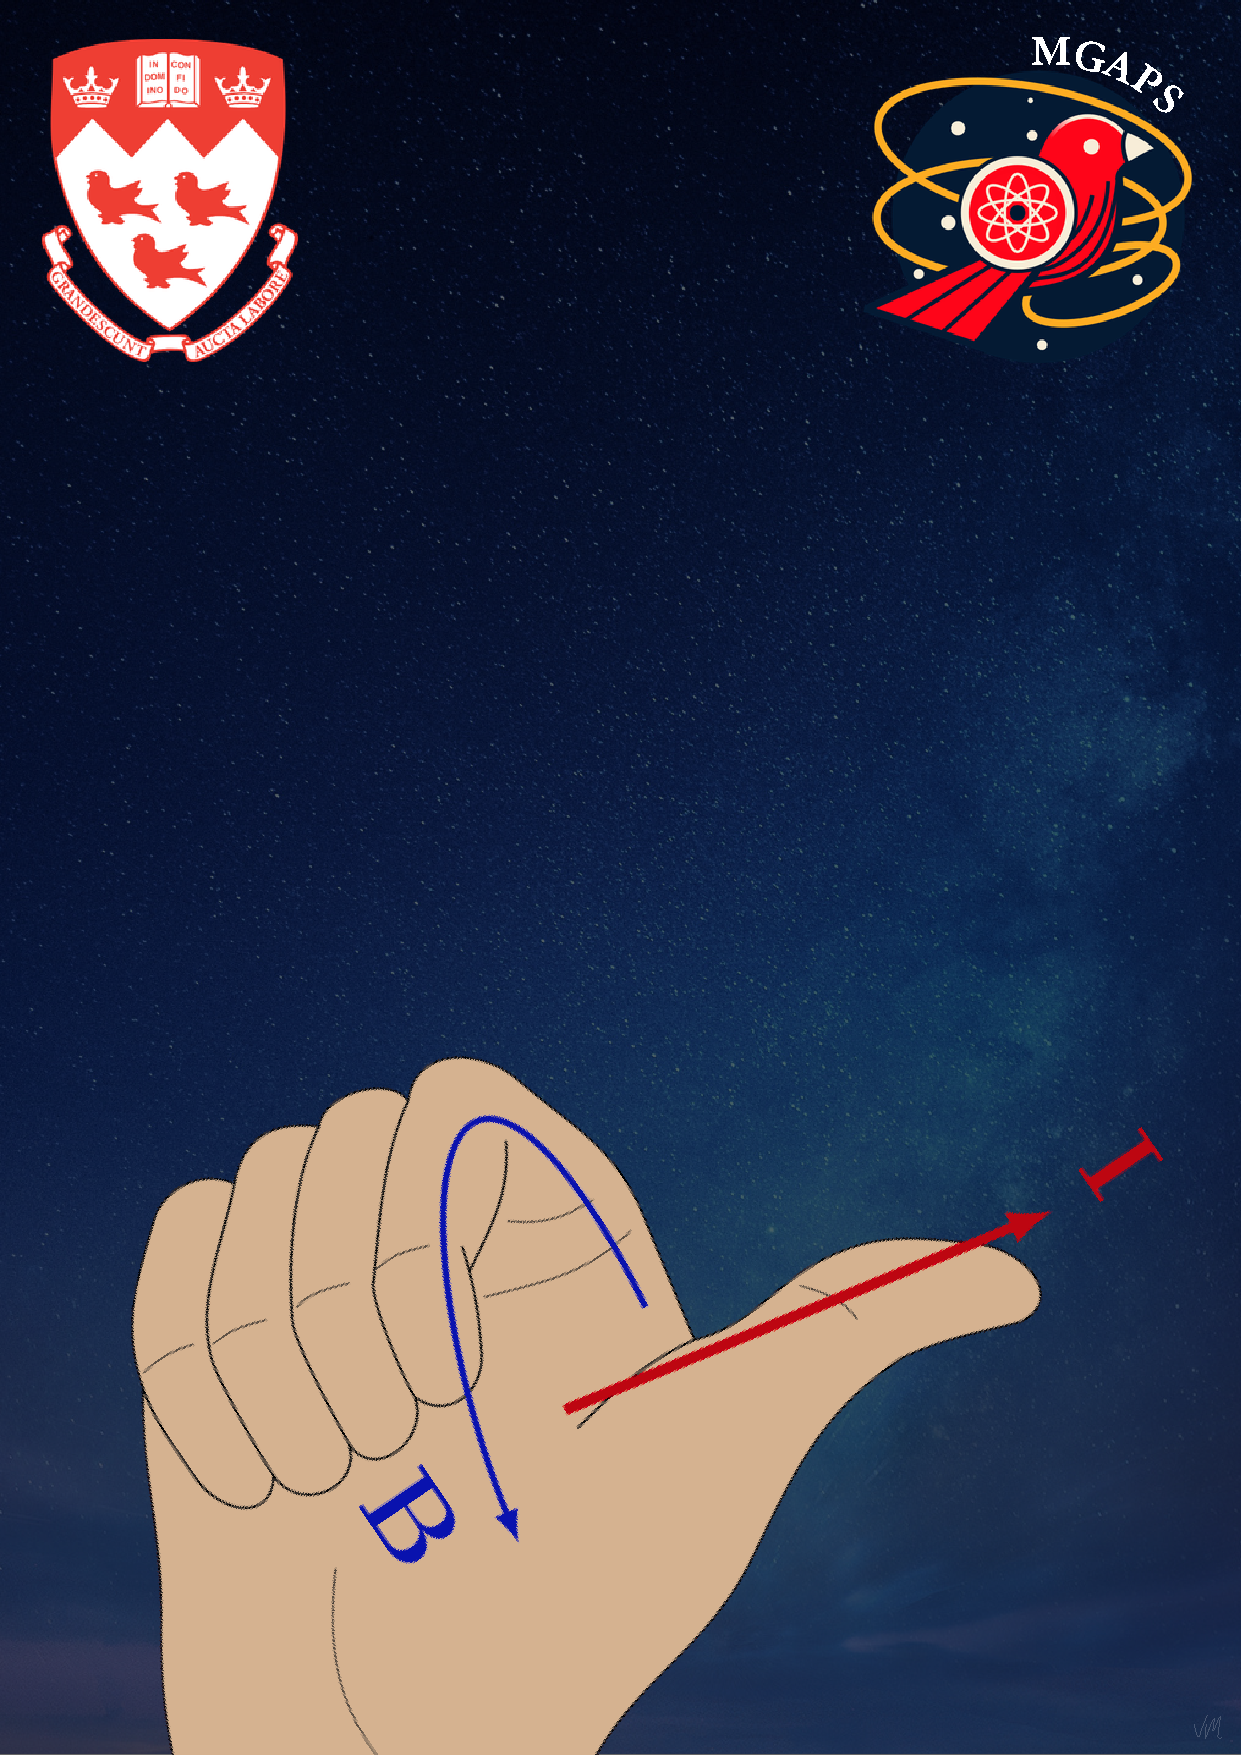
\includegraphics[width=\paperwidth]{cover}}; % Background image
\draw[anchor=north] (midpoint) node [fill=red!50!red,fill opacity=0,text opacity=1,inner sep=0cm]{\centering\bfseries\parbox[c][][t]{\paperwidth}{\hspace{-0.5cm}\centering \titlefont\Huge	\scalefont{2.5}\shadowtext{{\color{white}\textit{The Hitchhiker's}}}\\[1pt] % Book title
{\hspace{-1.5cm}\titlefont\Huge\scalefont{2.5}\shadowtext{{\color{white}\textit{Guide to McGill}}}}\\ [1pt] 
{\hspace{-9.5cm}\Huge\scalefont{2.5}\shadowtext{{\color{white}\textit{\raggedleft Physics}}}}}}; % Author name
\node[anchor=south east, inner sep=4pt,
        fill=black, fill opacity=0, text opacity=1,
        rounded corners=2pt] at (\paperwidth -1cm, -27cm)
    {\scalefont{2}\sffamily\color{yellow!50}\textit{a handbook}};
\end{tikzpicture}};
\end{tikzpicture}
\endgroup

\let\cleardoublepage\clearpage


 % Table of contents heading image
\chapterimage{contents.pdf}
\chapterimagecaption{\textit{The Village Lawyer’s Office} (1618) by Pieter Brueghel the Elder}
%\pagestyle{empty} % No headers
\tableofcontents % Print the table of contents itself

\cleardoublepage % Forces the first chapter to start on an odd page so it's on the right

\pagestyle{fancy} % Print headers again

%----------------------------------------------------------------------------------------
%	PART
%----------------------------------------------------------------------------------------


%----------------------------------------------------------------------------------------
%	CHAPTER 1
%----------------------------------------------------------------------------------------

% Chapter heading image
\chapterimage{onboarding.pdf}
\chapterimagecaption{\textit{The School of Athens} (1511) by Raphael}
\chapter{Onboarding}
    \section{Onboarding Checklist} \index{Onboarding}
Welcome to McGill! Below is a checklist for new students. Make sure to go over these items! This will make your life much easier.

\begin{itemize}[
    label={$\square$},
    leftmargin=1.8em,
    itemsep=1em
]

    \item Register as a \textbf{``full-time''} student by adding the Registration Confirmation course (REGN RCGR) for both the Fall and Winter terms. The registration period is until \textbf{August 14th, 2026}. Classes begin on \textbf{August 31st}. The Add/Drop deadline is \textbf{September 15th}.
    
    \item MSc students register for 30 research credits towards their thesis and 15 credits of courses. Typically, \textbf{PHYS 693} is taken in the 1st year with courses; \textbf{PHYS 690D1} and \textbf{PHYS 690D2} are taken in the 2nd year.

    \item PhDs take two classes at the 600+ level. Students who complete their MSc at McGill can carry over one of the 600+ level courses. PhDs must also pass the \textbf{PhD Preliminary Exam}.

    \item Additionally, new students must also take two professional development courses, \textbf{PHYS 601 \& 602}. 

    \item Check your official McGill e-mail account (first.last@mail.mcgill.ca) for announcements, scholarship opportunities and formal paperwork.

    \item Request a \textbf{Tuition Deferral} in Minerva to avoid interest charges on your student account. Tuition supplements can only be paid out on September 1st.

    \textit{Minerva > My Financial Aid \& Awards > Defer Payment of Tuition \& Fees.}

    \item \textbf{Conditions of Admission:} Submit your final official transcripts/proof of graduation to Enrolment Services. Many universities are now providing electronic copies. They can be sent to \href{mailto:officialschooldocs@mcgill.ca}{officialschooldocs@mcgill.ca}.

    \item \textbf{International students:}  Keep the department updated and let them know when you receive your \textbf{CAQ} and \textbf{Study Permit}. Use \href{https://www.mcgill.ca/legaldocuments/how}{this} site for information on uploading your documents. When you arrive in Canada, you will open a Canadian bank account and update your mailing address in Minerva. You have options for receiving your research stipend before you arrive in Canada. \\    

    \textbf{\color{ocre}Note:} When you arrive in Canada, you can request an adjustment (or refund) for the \textbf{International Health Insurance premium}, for the months that you were not in Canada. \index{Health Insurance!International Health Insurance}

    \item \textbf{Canadian students:} Update your personal banking information in Minerva to set up your \textbf{Direct Deposit}. 
    
    \item Send your signed \textbf{TA contract} and personal data form to Kim (\href{mailto:ao.physics@mcgill.ca}{ao.physics@mcgill.ca}), so that she can create your TA appointment in Workday.

     \item \textbf{Finding a desk:} You must make sure to set up an office space from where you can work, this procedure may vary slightly from student to student depending on their group, see the next section for more details. Email Kim when you have a desk, for access.
     
     \item \textbf{Building access:} As an active member of the physics community, you should make sure you have keycard access to your lab, office, and the Rutherford Physics Building. Since Louise has retired, reach out to Robert Turner (\href{mailto:robert.turner@mcgill.ca}{robert.turner@mcgill.ca}) to request keycard access.

    \item Email the Graduate Coordinator, Sam Maroussis (\href{mailto:Graduate.Physics@McGill.ca}{Graduate.Physics@McGill.ca}) if you have any questions!

\end{itemize}

\medskip

\textbf{\color{ocre}Note:} you will also receive this checklist from Sam to help you get set up.

\subsection*{McGill E-Mails}\index{Emails}
\begin{itemize}
    \item You have a McGill email: 
    \href{mailto:first.last@mail.mcgill.ca}{first.last@mail.mcgill.ca}.

    \item You can get an account on the department Linux network (ask your supervisor) which will give you an @physics.mcgill.ca e-mail.

    \item If you are a teacher assistant (TA), you will also be assigned an e-mail which is 
    \href{mailto:@mcgill.ca}{@mcgill.ca}. Note that this is temporary! It will go away if you stop being a TA, such as during the summer or during terms where you have a TA buyout from your supervisor. 
    \item To avoid the failure mode where you cannot access emails sent to your @mcgill.ca emails during times when this email is deactivated, consider setting up Outlook forwarding from your @mcgill.ca to @mail.mcgill.ca account.
\end{itemize}

It’s really important to check your McGill email (@mail.mcgill.ca) -- this is where announcements about things like funding, workshops will come. You should also use it for communication within the university (you may not get a response otherwise). Department announcements can sometimes go to your physics email address \href{mailto:grads@physics.mcgill.ca}{grads@physics.mcgill.ca} (if you have one). You can have this redirected to your McGill email address by adding a \texttt{.forward} file in your home directory, or if you don’t have a physics account you can email Juan Gallego \href{mailto:operator@physics.mcgill.ca}{(operator@physics.mcgill.ca)} to make one.

\subsection*{ID Cards}\index{ID Cards}
To get your McGill ID, follow the steps on \href{https://www.mcgill.ca/student-records/personal-information/id}{this} website. You just need to upload your photo using the upload tool, wait for it to get approved, and then collect it from Service Point.

\subsection*{Building Access}\index{Building Access}
There are many different types of access within the Rutherford Physics Building. Access can be requested only after the ID card has been physically picked up by the student. They must send Robert Turner an email indicating their name, email, and the room for which access is requested, while CCing their supervisor. 

All graduate students are guaranteed after-hour access to the building. Send another mail to Robert (without CCing your supervisor) with your McGill ID and a PIN. To open Rutherford doors after-hours, tap your keycard on the reader in the main entrance and type the \textbf{\color{ocre} last four digits} of your student ID number or the PIN of your choosing. Access to specific offices must be requested directly from the administration. 

In case your work requires access to your group's laboratory space, contact your supervisor and the administration. To access specific research facilities and creative spaces within the Rutherford and Wong buildings, such as the Wet Lab or the Makerspace, you must contact the technician responsible for the site to obtain access. Rooftop access is restricted to individuals working with the Anna McPherson observatory or who work with research materials stored on the roof.


\subsection*{Getting a Desk} \index{Finding a Desk}
The most direct and most commonly used way to secure a desk in the Rutherford Physics Building offices is to pick the office of your choice and check with the current occupiers if there are any desks available. Once you have found a free desk, make sure to claim it by attaching a name tag to it: simply write your name and contact information. Afterwards, contact Kim Metera (\href{mailto:ao.physics@mcgill.ca}{ao.physics@mcgill.ca}) with your room and desk number.

\begin{plainexercise}
 Note that even if you claim a desk by adding your name tag, you must make sure to actively use it otherwise it is entirely possible someone else will claim it as their own.    
\end{plainexercise}
\vspace{-5pt}
Some research groups have desks inside their laboratories, in which case you should check with your group mates to check if any of those desks are available. Do \textbf{NOT} claim multiple desks in the building, desk space is limited and cases of double-desking will inevitably lead you to get kicked out of one of your desks.

Recently, the MGAPS council is mounting a Graduate Study Room in ERB 433, featuring communal desks equipped with monitors. This initiative is meant to accomodate any students that do not have a permanent desk and are on the desk waitlist, which is especially the case for incoming students.

\subsection*{Room Booking} \index{Room Booking}
To book a room in the Rutherford, contact Maha (\href{mailto:chairsec.physics@mcgill.ca}{chairsec.physics@mcgill.ca}) for now. All room bookings are detailed on \href{https://calendar.google.com/calendar/u/0/embed?height=600&wkst=1&bgcolor=%23ffffff&ctz=America/Toronto&src=bG91aXNlLmRlY2VsbGVzQG1jZ2lsbC5jYQ&src=cGh5c2ljc3Jvb21zQGdtYWlsLmNvbQ&color=%23039BE5&color=%23039BE5}{this calendar}, consult it to verify which rooms are available. Note that if you wish to book the Rutherford Auditorium (ERB 112), you must submit a request to the McGill Faculty of Science.

\subsection*{Safety and Training}\index{Safety}
The Department Safety Committee (DSC) is responsible for ensuring safety standards within the Rutherford Physics Building. Primarily, this includes laboratory safety, disposal of laboratory materials and junk, construction, and building operation (e.g. shut downs and leaks). The Chair and Safety Officer, Michael Hilke, is primarily responsible for ensuring these safety standards. Matters such as junk removal, on-going construction, and maintenance are usually handled by the Building Director, Andreas Warburton. 

The Environmental Health and Safety (EHS) is the entity responsible for training and certifying laboratory personnel. Any research involving laboratory work requires EHS certification and safety training, and some types of work (e.g. radiation, lasers) may require further training and permits.

For more on the role of the DSC, please see \href{https://www.mcgill.ca/ehs/policies-and-safety-committees/health-and-safety-committees/departmental-safety-committees}
{here}. For more information regarding the EHS, see \href{https://www.mcgill.ca/ehs/training}{here}. Also, contact your supervisor for more information regarding your own laboratory safety procedures and certifications.

\section{Relevant Contacts} \label{contacts}

\subsection*{Administration, Advisors, and Committee Chairs}
Below is a comprehensive list of the administration team, their roles, and contacts (as of August 2026).

\vspace{-5 pt}
    \begin{table}[h!]
        \hspace*{-1.5cm}
    \centering
    \renewcommand{\arraystretch}{1.2}
    \arrayrulecolor{ocre}
    \begin{tabular}{|>{\columncolor{ocre!20}}lc>{\columncolor{ocre!20}}cc|}
    \hline
    \rowcolor{ocre!60}
  {\color{white}\large\sffamily \textbf{Role}} & {\color{white}\large\sffamily \textbf{Name}}  & {\color{white}\large\sffamily \textbf{Office}}  & {\color{white}\large\sffamily \textbf{Email Address}} \\
        Department Chair & Ken Ragan & ERB 108 & chair.physics@mcgill.ca\\
        Building Director & Andreas Warburton & ERB 343 & buildingdirector.physics@mcgill.ca \\
        Safety Officer & Michael Hilke & ERB 408 & michael.hilke@mcgill.ca \\
        Administrative Officer & Kim Metera & ERB 108 & ao.physics@mcgill.ca \\
        Graduate Studies Coordinator & Sam Maroussis & ERB 108 & graduate.physics@mcgill.ca \\
        Graduate Studies Advisor & Nikolas Provatas & ERB 218 & nikolaos.provatas@mcgill.ca \\
        Undergraduate Advisor & Maha Ibrahim & ERB 223 & advising.physics@mcgill.ca \\
        Reimbursements \& Financials & Sonal Patel & ERB 443 & scipod1.managers@mcgill.ca \\
        Administrative Coordinator & Eddie Del Campo & ERB 108 & eduardo.delcampo@mail.mcgill.ca \\
        Administrative Coordinator & Alba Furfaro & ERB 108 & alba.furfaro@mcgill.ca \\
        Computer System Operator & Juan Gallego & ERB 331 & juan.gallego@mcgill.ca \\
        Library Liaison & April Colosimo & & april.colosimo@mcgill.ca \\
        EDI Committee Chair & Jason Hessels & ERB 215 & jason.hessels@mcgill.ca \\
        Inreach/Outreach Coordinator & Eesha Das Gupta & TSI 030A & eesha.dasgupta@mcgill.ca \\
        \hline
\end{tabular}
\arrayrulecolor{black}
\end{table}

\subsection*{Technicians and Professionals}   
Below is a table containing all technicians and research professionals affiliated with the Physics Department (as of August 2026). In case you require assistance, contact your supervisor to determine the best way to proceed and the best suited research professional.

\vspace{-5 pt}
 \begin{table}[h!]
        \hspace*{-1.7cm}
    \centering
    \renewcommand{\arraystretch}{1.2}
    \arrayrulecolor{ocre}
    \begin{tabular}{|>{\columncolor{ocre!20}}lc>{\columncolor{ocre!20}}cc|}
    \hline
    \rowcolor{ocre!60}
  {\color{white}\large\sffamily \textbf{Role}} & {\color{white}\large\sffamily \textbf{Name}}  & {\color{white}\large\sffamily \textbf{Office}}  & {\color{white}\large\sffamily \textbf{Email Address}} \\

        Linux Support and Physics Servers & Juan Gallego & ERB 331 & juan.gallego@mcgill.ca \\
        Machine Shop Supervisor & Pascal Bourseguin & ERB 004 & pascal.bourseguin@mcgill.ca \\
        Machine Shop Technician & Marc Giroux & ERB 004 & marc.giroux@mcgill.ca \\
        Electronics Design & Eamon Egan & ERB 228 & eamon.egan@mcgill.ca \\
        Rutherford Sample Preparation Lab &  Robert Gagnon & ERB 421A & robert.gagnon@mcgill.ca \\
        Technician: Vacuum Systems & John Smeros & ERB 420B & john.smeros@mcgill.ca \\
        Technician: Electronics Support & Richard Talbot & ERB 422A & richard.talbot@mcgill.ca \\
        Technician: Windows Support & Janney Wu & WON 0130 & janney.wu@mcgill.ca \\
        Undergraduate Lab Manager & Robert Turner & WON 0121 & robert.turner@mcgill.ca \\
        Technician: Undergrad Teaching Lab  & Anwesha Basu & Trottier 3080 & anwesha.basu@mcgill.ca \\
        Technician: Undergrad Teaching Lab  & Robert Idsinga & WON 0101 & robert.idsinga@mcgill.ca \\
        Technician: Undergrad Teaching Lab  & Philippe Movafegh & WON 0130 & philippe.movafegh@mcgill.ca \\
        Technician: Undergrad Teaching Lab & Brandon Ruffolo & WON 0130 & brandon.ruffolo@mcgill.ca \\
        Nanotools Manager & Zhao Lu & ERB 014 & zhao.lu@mcgill.ca \\
        Nanotools Equipment Technologist & John Li & ERB 013 & john.li@mcgill.ca \\
        Nanotools Research Professional & Peng Yang & ERB 013 & peng.yang2@mcgill.ca \\
        \hline
\end{tabular}
\arrayrulecolor{black}
\end{table}
\newpage

\subsection*{Wider University} 
Below is a list of contacts for individuals within McGill that could prove useful (as of August 2026).
\vspace{-5 pt}
 \begin{table}[h!]
        \hspace*{-1.7cm}
    \centering
    \renewcommand{\arraystretch}{1.2}
    \arrayrulecolor{ocre}
    \begin{tabular}{|>{\columncolor{ocre!20}}lc>{\columncolor{ocre!20}}cc|}
    \hline
    \rowcolor{ocre!60}
  {\color{white}\large\sffamily \textbf{Role}} & {\color{white}\large\sffamily \textbf{Name}}  & {\color{white}\large\sffamily \textbf{Site}}  & {\color{white}\large\sffamily \textbf{For Appointments}} \\

        Dean of Students & Tony Mittermaier & \href{https://mcgill.ca/deanofstudents/}{Link}& deanofstudents@mcgill.ca \\
        Dean of Graduate and Post-Doctoral Studies & Marie-Hélène Pennestri & \href{https://mcgill.ca/gps/}{Link}& Deanadm.gps@mcgill.ca \\
        Dean of Science & Alana Watt & \href{https://mcgill.ca/science/}{Link} & secdean.science@mcgill.ca \\
        \hline
\end{tabular}
\arrayrulecolor{black}
\end{table}


\section{Getting Involved}
\subsection{McGill Graduate Association of Physics Students (MGAPS)} \index{MGAPS}
The McGill Graduate Association of Physics Students (MGAPS) is the official division of all graduate physics students at McGill University. In other words, every graduate student is an MGAPS member. A \$10 fee for MGAPS membership is automatically billed into the graduate student tuition by the Post-Graduate Student Society (comprised of all graduate student associations in McGill University) into the MGAPS yearly budget for the organization of actions and events that aim to improve graduate students' experiences. The MGAPS council is a group of elected volunteers that serves as the governing body of MGAPS and is comprised of a president, vice-presidents, officers, representatives, and liaisons (for a full list of these roles and their descriptions see the \href{https://mgaps.physics.mcgill.ca/people/}{list of current council members} or the \href{https://mgaps.physics.mcgill.ca/files/MGAPS_Constitution_2025-01-28.pdf}{constitution}). The MGAPS council has as primary objectives the maintenance and improvement of wages, infrastructure, and enrichment for MGAPS members. 

\begin{plaincorollary}
    Becoming involved with the MGAPS council and MGAPS events is one of the most direct ways for graduate physics students to meet new people, develop leadership skills, and learn how to navigate new research environments.
\end{plaincorollary}
To become involved with MGAPS and the council, the council meets on a \textbf{biweekly basis} and organizes a series of weekly and recurring events, all details of which are noted in the \href{https://mgaps.physics.mcgill.ca/community/events/}{MGAPS calendar}). All MGAPS council activities and meetings are open to all MGAPS members. The MGAPS council also maintains the \textbf{Graduate Student Lounge (ERB 322)}, located in the 3rd floor of the Rutherford Physics Building, as a social space for all graduate students and post-docs in physics, and the lounge operates as the primary locations for council meetings and small MGAPS events. Any member of MGAPS can assume a position within the MGAPS council by winning the elections hosted in the Fall MGAPS General Assemblies, and any vacant positions will be again open for election in the Winter MGAPS General Assemblies as per the \href{https://mgaps.physics.mcgill.ca/files/MGAPS_Constitution_2025-01-28.pdf}{constitution}.
\begin{plainexercise}
    The MGAPS council is involved with various bodies both in and out of McGill University, including: Physics department administration, the Physics research centers (CHEP, CPM, and TSI), the Equity, Diversity, and Inclusion Committee, the Outreach Committee, the Teaching Support Union at McGill, the Post-Graduate Student Society, the Faculty of Science, and industry.
\end{plainexercise}
So, if you are interested, get involved with the MGAPS council! In order to contact any MGAPS council see the contacts listed below or see the \href{https://mgaps.physics.mcgill.ca/people/}{list of current council members} for specific contacts. Join the MGAPS Slack \href{https://mcgillphysics-rag1431.slack.com/join/shared_invite/zt-3vlrg6luf-k0KqSG3LdCQ2V2P96XF_kQ#/shared-invite/email}{here}.

\vspace{-5 pt}
 \begin{table}[h!]
    \centering
    \renewcommand{\arraystretch}{1.2}
    \arrayrulecolor{ocre}
    \begin{tabular}{|l>{\columncolor{ocre!20}}cc|}
    \hline
    \rowcolor{ocre!60}
  {\color{white}\large\sffamily \textbf{Role}} & {\color{white}\large\sffamily \textbf{Name}} &{\color{white}\large\sffamily \textbf{Email}} \\

        President and Vice Presidents & MGAPS & mgaps.exec@physics.mcgill.ca \\
        \hline 
\end{tabular}
\arrayrulecolor{black}
\end{table}
Note that it may be more practical to reach out to specific contacts.

\subsection{McGill Society of Physics Students (MSPS)}
The McGill Society of Physics Students (MSPS) is the official division of all undergraduate physics students at McGill University. Therefore, all undergraduate physics students are members of MSPS, and MSPS is an organization within the Students’ Society of McGill University. The MSPS council is a volunteer group of undergraduates that is elected as the representative body of MSPS, and a full list of the roles and their descriptions can be found in the \href{https://www.msps.physics.mcgill.ca/}{MSPS website}. The MSPS council maintains the Undergraduate Student Lounge as a social space for undergraduates, and MSPS council meetings take place in this lounge. The MSPS collaborates with MGAPS, the Equity, Diversity, and Inclusion Committee, and the Outreach Committee in the organization of events. The MSPS council is also the primary body within the physics department that is responsible for ordering McGill Physics merchandise for both undergraduate and graduate students, orders are handled seasonally by MSPS and can be ordered through the \href{https://www.msps.physics.mcgill.ca/}{MSPS website}. To contact the MSPS council, see the contacts listed below or see the \href{https://www.msps.physics.mcgill.ca/}{MSPS website} for specific contacts.

\vspace{-5 pt}
 \begin{table}[h!]
    \centering
    \renewcommand{\arraystretch}{1.2}
    \arrayrulecolor{ocre}
    \begin{tabular}{|l>{\columncolor{ocre!20}}cc|}
    \hline
    \rowcolor{ocre!60}
  {\color{white}\large\sffamily \textbf{Role}} & {\color{white}\large\sffamily \textbf{Name}}   & {\color{white}\large\sffamily \textbf{Contact}} \\

        President and Vice Presidents & MSPS & msps.physics@mcgill.ca \\
        \hline
\end{tabular}
\arrayrulecolor{black}
\end{table}
Note that it may be more practical to reach out to specific contacts.

\subsection{Equity, Diversity, and Inclusion (EDI) Committee} \index{Coordinators!EDI}
The Equity, Diversity, and Inclusion (EDI) Committee in the Department of Physics at McGill is a group of students, postdoctoral fellows, staff, and faculty members that aims to create a safe and inclusive working environment. The EDI Committee seeks to achieve this by organizing social and educational events, participating in outreach with CÉGEPs, maintaining EDI-related resources, and organizing with the physics administration team to improve departmental policies and conditions. The committee is led by a chair and composed of members, all of which are listed in the \href{https://www.physics.mcgill.ca/edi/}{EDI Committee website}, and frequently collaborate with MGAPS and MSPS. 

To become involved with committee activities, students can attend the \textbf{weekly Physics and Society Discussion Group} to discuss topics suggested by students and special EDI events announced by the committee. The committee also organizes a \textbf{weekly lunch for women and non-binary people} in physics in the Graduate Student Lounge (ERB 322), and the lunch is catered on a biweekly basis. Finally, the EDI Committee organizes an \href{https://www.physics.mcgill.ca/edi/library.html}{Equity Library} on the 2nd floor of the Rutherford Physics Building that covers equity issues in Canada and the United States. See the MGAPS Newsletter or the \href{https://www.physics.mcgill.ca/edi/events.html}{EDI Committee events page} for more details on recurring EDI events and resources.

To become a member of the EDI Committee, students may apply for one of the two paid \textbf{Graduate EDI Coordinator} positions open for graduate students (the pay is equivalent to a teaching assitant position) or be elected for the EDI Officer position within the MGAPS council. To contact the EDI Committee, see the contacts listed below or see the \href{https://www.physics.mcgill.ca/edi/}{EDI Committee website} for more specific contacts.

\vspace{-5 pt}
 \begin{table}[h!]
        \hspace*{-1.2cm}
    \centering
    \renewcommand{\arraystretch}{1.2}
    \arrayrulecolor{ocre}
    \begin{tabular}{|>{\columncolor{ocre!20}}lc>{\columncolor{ocre!20}}c|}
    \hline
    \rowcolor{ocre!60}
  {\color{white}\large\sffamily \textbf{Role}} & {\color{white}\large\sffamily \textbf{Name}}   & {\color{white}\large\sffamily \textbf{Contact}} \\

        EDI Committee Chair & Jason Hessels & jason.hessels@mcgill.ca \\
        Graduate EDI Coordinator & Angela Sabzevari Gonzalez & angela.sabzevarigonzalez@mail.mcgill.ca \\
        Graduate EDI Coordinator & Maryam Rahbaran & maryam.rahbaran@mail.mcgill.ca \\
        EDI Officer & Jack Faller & jacob.faller@mail.mcgill.ca \\
        \hline
\end{tabular}
\arrayrulecolor{black}
\end{table}

\subsection{Outreach Committee: McGill Physics and TSI Outreach} \index{Coordinators!Outreach}
The McGill Physics and TSI Outreach Committee is the primary organizing body behind outreach and science communication initiatives in the Physics department, and is composed of the McGill Physics and the Trottier Space Institute (TSI) outreach teams. The Outreach Committee aims to communicate Physics and Astronomy research to the general public, students, and the McGill community, and counts on the participation of paid outreach coordinators (the salary being roughly equivalent to a teaching assistantship) and numerous volunteers. 

To become members of the Outreach Committee, graduate students can become \textbf{outreach coordinators} by applying for the positions. Alternatively, graduate students can also become members by being elected as VP Professional Development in the MGAPS Council, who acts as a liaison between the committee and the MGAPS council. The Outreach Committee frequently calls upon volunteers from both graduate and undergraduate student bodies to organize its events, and it is an excellent way to begin involvement in outreach. To contact the Outreach Committee, see the contacts listed below or see the \href{https://physics-tsi-outreach.physics.mcgill.ca/index.html#team}{Outreach Committee website} for more specific contacts. Join the Outreach Slack to check for department-wide activity.

\vspace{-5 pt}
 \begin{table}[h!]
        \hspace*{-2.7cm}
    \centering
    \renewcommand{\arraystretch}{1.2}
    \arrayrulecolor{ocre}
    \begin{tabular}{|>{\columncolor{ocre!20}}lc>{\columncolor{ocre!20}}c|}
    \hline
    \rowcolor{ocre!60}
  {\color{white}\large\sffamily \textbf{Role}} & {\color{white}\large\sffamily \textbf{Name}}   & {\color{white}\large\sffamily \textbf{Contact}} \\

        Outreach Committee Chair & Thomas Brunner & outreach@physics.mcgill.ca \\
        Outreach Coordinator & Eesha Das Gupta & eesha.dasgupta@mcgill.ca\\
        Public Talks and Social Media Coordinator & Amélie Chiasson David & amelie.chiassondavid@mail.mcgill.ca\\
        Public Observing Nights & Anna I. McPherson Observatory & observatory@physics.mcgill.ca  \\
        Hackathon Coordinator &  Brendan Barry & hackathon@physics.mcgill.ca \\
        Space Explorers Coordinator & Patrick Horlaville & patrick.horlaville@mail.mcgill.ca \\
        Science in Space Coordinator & Georgia Mraz & georgia.mraz@mail.mcgill.ca \\
        MGAPS Liaison & Catherine Boisvert & catherine.boisvert4@mail.mcgill.ca\\
        \hline
\end{tabular}
\arrayrulecolor{black}
\end{table}

\newpage
\subsubsection{Public Talks} \index{Coordinators!Public Talks}
The Physics Department offers public talks roughly monthly during the academic year. Speakers are often professors, permanent researchers, postdocs, or senior PhD students-including researchers from local institutions and visiting scholars alike. The McGill Physics and TSI Public Talks are organized by a paid Outreach Coordinator (see contact above). Some volunteer opportunities include helping guide members of the public, posting and removing signs, and staffing the book sale table (if applicable). 

\subsubsection{Public Observing Nights and Events} 
The Anna McPherson observatory is located on the fifth floor of the Rutherford Building and hosts \textbf{monthly public observing nights} as well as other outreach and inreach events. The observatory coordinator is (historically) a graduate student volunteer role and the events are supported by undergraduate, graduate, postdoc, and staff volunteers who help operate telescopes and talk to the public about astronomy, current events in space, and astro-related research at McGill. Anyone in the department is welcome to volunteer for events, no prior experience required! Please email \href{mailto:observatory@physics.mcgill.ca}{observatory@physics.mcgill.ca} to be added to the volunteer list. The observatory coordinator monitors this inbox, but you can also (secondarily) reach out to the TSI inreach/outreach coordinator.  

The Outreach Committee often hosts outreach observation events during eclipses, such as providing educational materials and safe viewing methods for the 2026 partial, 2024 total solar eclipses, and rooftop observations of lunar eclipses (such as in 2025). These events are, naturally, seasonal and community involvement varies depending on the magnitude of the eclipse. For instance, the 2024 total solar eclipse was effectively a mass mobilization effort requiring total committee involvement, multiple graduate and undergraduate volunteers, an information fair, and featured a full crowd of visitors occupying the entire McGill Campus. Therefore, these events may require a large or small group of volunteers depending on popular demand.

\subsubsection{McGill Physics Hackathon}\index{Coordinators!Hackathon}
The McGill Physics Hackathon started in 2016 and is an annual computer programming competition open to anyone (and especially attended by undergraduate, CÉGEP, and high school students). The hackathon is an extensive endeavour, and organization efforts are led by the \textbf{Hackathon Outreach Coordinator} and the hackathon team. The hackathon also counts on the assistance of a team of volunteers, and is a popular way to become involved with science education and project development. To learn more about the physics hackathon, see the \href{https://www.hackathon.physics.mcgill.ca/}{McGill Physics Hackathon website}.

\subsubsection{Space Explorers}\index{Coordinators!Space Explorers}
Space Explorers is an Outreach Committee initiative through which recruited and trained volunteers visit elementary school classrooms to deliver hands-on, inquiry-based learning activities meant to initiate children to fundamental physics concepts (such as density, gravity, craters, and friction). These activities are designed for children aged 9-10 (grades 3-4) but can extend to younger (grade 2) and older (grades 5-6) children in some cases. Through Space Explorers, volunteers gain experience in teaching to children and developing their science communication skills, some activities may be in French so it might be an opportunity to practice.

\subsubsection{Science in Space} \index{Coordinators!Science in Space}
“Science in Space (in collaboration with Dell Technologies/Girls who Game) is a 10-week astronomy program introducing elementary students (grades 5-8; ages 10-14) to physics, astronomy, and telescopes. Students learn about telescopes through hands-on lessons, and ultimately design and build telescopes in Minecraft with the guidance of graduate student mentors (who themselves identify as members of marginalized groups in STEM). Science in Space is organized by the Science in Space Outreach Coordinator (see contact above). The program is aimed at girls and students of marginalized genders in STEM to mitigate attrition from STEM”.

\subsubsection{Science Fairs, Open Houses, and Tours}
There are many opportunities to volunteer at city-wide science fairs through the Outreach Committee, such as Family Science Day in September, and 24 Heures de Science in May, and AstroFest. Volunteer duties vary but often include ``classic" outreach activities relating to building a solar system mobile, aluminium foil boats, designing an extremophile, straw rockets, craters, constellations, and more. The physics department also has working relationships with several schools. For example, there is often demand for judges for the Royal Vale School science fair in the spring, and there is demand for outreach volunteers to work with ``World of STEM" participants.

Sometimes physics department members organize open houses to invite high school groups to learn more about the department, tour the Rutherford Physics Collection Museum (see below). In such cases, physics department members often seek a small group of graduate students to give brief talks about their research. 

Lastly, some laboratories and groups conduct their own outreach opportunities (e.g. the RAD kits designed by the McGill Radio Lab). Ask around to learn more!

\subsubsection{The Ground State Podcast (MGAPS)}
The Ground State Podcast is a recent outreach initiative started by the MGAPS council. \textbf{Note} that the podcast is \textbf{NOT} an Outreach Committee initiative but it is coordinated by the MGAPS liaison within the Outreach Committee, who serves as VP Professional Development within the MGAPS council. The podcast interviews students about their work with the aim of giving more visibility to the research done within the physics department. Specifically, the podcast primarily interviews students about published work and their experiences. If you wish to participate in the podcast initiative or be interviewed, reach out to the MGAPS liaison within the Outreach Committee.


\subsection{Departmental Divisions}
The McGill Physics Department is host to various research centers covering the primary research interests of the physics community. Many students within the physics department work primarily within one or multiple of these centers and their facilities. The MGAPS council is currently seeking to arrange a meeting of center organizers once a year to maintain an open communication channel between the centers.  

\subsection*{Center for High Energy Physics (CHEP)}\index{CHEP}
The Center for High Energy Physics (CHEP) is the primary center for people working in high energy and nuclear physics and is composed of subgroups in experimental high energy physics (XHEP), theoretical high energy physics (THEP), nuclear physics (NP), and particle astrophysics (PA). Founded in 1983, the CHEP is hosted in the \textbf{3rd level of the Rutherford Physics Building}, and features seminars and journal clubs covering its community's research interests including: Hadronic Physics Seminars, Particle and Astroparticle Seminars, Theory HEP Seminars, and HEP Theory Journal Club. 

The CHEP consists of faculty members affiliated with CERN, SNOLAB, TRIUMF, VERITAS, and RHIC, as well as a roster of \href{https://www.physics.mcgill.ca/chep/ras-f.html#XHEP}{research associates} and visiting scholars from various research centers and universities. The CHEP is also responsible for hosting the \href{https://www.physics.mcgill.ca/~francois/projects/guidelines.html}{Physics Computer Network}, which is utilized by various groups in the physics department including the CPM and the TSI. Researchers also frequently use clusters at the Digital Research Alliance of Canada (DRAC; formerly Compute Canada) to run demanding programs.

The CHEP is organized primarily by its faculty members, usually through the lead of a director, and seminars are run by select post-docs and doctoral students. The XHEP branch is also involved in organizing outreach initiatives, in collaboration with the Outreach Committee, including LEGO models, spark chambers, bubble chambers, and tours, see \href{https://www.physics.mcgill.ca/xhep/en/outreach/}{here} to learn more. For more information on the CHEP, see the \href{https://www.physics.mcgill.ca/chep/}{CHEP page} and see contacts below for faculty members primarily involved with CHEP organization. See also the \href{https://www.physics.mcgill.ca/xhep/en/}{XHEP} page for more information on experimental research. \textbf{Note} that the CHEP is currently in a transitional state following the retirement of its previous director so the contacts below are \textit{de facto} organizers. 

\vspace{-5 pt}
 \begin{table}[h!]
    \centering
    \renewcommand{\arraystretch}{1.2}
    \arrayrulecolor{ocre}
    \begin{tabular}{|>{\columncolor{ocre!20}}lc>{\columncolor{ocre!20}}c|}
    \hline
    \rowcolor{ocre!60}
  {\color{white}\large\sffamily \textbf{Role}} & {\color{white}\large\sffamily \textbf{Name}}   & {\color{white}\large\sffamily \textbf{Contact}} \\

        Faculty Member & Thomas Brunner & thomas.brunner@mcgill.ca \\
        Faculty Member & Brigitte Vachon & brigitte.vachon@mcgill.ca \\
        
        \hline
\end{tabular}
\arrayrulecolor{black}
\end{table}



\subsection*{Center for the Physics of Materials (CPM)}\index{CPM}
The Center for the Physics of Materials (CPM) was funded in 1989 and is the primary center for people working in condensed matter and materials physics. The center is present in the \textbf{4th level of the Rutherford Physics Building} and is funded by the \href{https://rqmp.ca/}{Regroupement Québécois sur les Matériaux de Pointe (RQMP)}, the Faculty of Science, and McGill University. The research scope of the center is incredibly broad and features members and associates from various departments including physics, chemistry, biology, computer science, materials engineering, electrical engineering, and chemical engineering. The center also employs research staff and technicians, and is directly involved with the \href{https://www.mcgill.ca/microfab/}{McGill Nanotools Micro- and Nanofabrication Facility} in the B1 level as well as the \href{https://www.physics.mcgill.ca/preplab/}{Sample Preparation Laboratory} (ERB 205-206) in the 2nd level of the Rutherford Physics Building.

The CPM is associated with three primary research networks: the RQMP, \href{https://www.intriq.org/}{Institut Transdisciplinaire d'Information Quantique (INTRIQ)}, \href{https://www.mcgill.ca/miam/}{McGill Institute for Advanced Materials (MIAM)}, and the McGill Quantum Center (MQC) (which is currently being built). Through these networks, CPM students attend student conferences including the Advanced Materials Academy (AMA) summer school, the INTRIQ seasonal conferences, MaQTech conferences, and the MQC conference. Through these networks, CPM members are able to utilize facilities in the Université de Montréal, the 
Polytechnique Montréal, and the Université de Sherbrooke, and coordinate internships with industry and other universities both in and out of Canada. Researchers also frequently use  clusters at the Digital Research Alliance of Canada (DRAC; formerly Compute Canada) to run demanding programs. Some CPM members also maintain third party affiliations within their own groups, one example being \href{https://nanoacademic.com/}{Nanoacademic Technologies}, and these affiliations serve as means for students to become involved with industry or other aspects of research. Beyond these affiliations, some CPM groups also collaborate and co-supervise with CHEP, TSI, and the Medical Physics Unit on particular projects.

The CPM is organized by a scientific directorship and a student committee, which organize weekly CPM seminars, the annual CPM day, and numerous social events, such as student talks and barbecues. The weekly CPM seminars feature invited speakers presenting research relevant to the center, while CPM Day is an annual conference organized by the CPM directorship and student committee. The student committee also coordinates the student talks, where students and postdoctoral researchers present and share their work with the CPM community. Any CPM student can become a member of the CPM committee and is encouraged to do so to contribute to community building. Given the interdisciplinary nature of the CPM, students involved with organizing will occasionally have to work with different institutes and departments. Students can volunteer to help organize CPM events, and volunteering work may include helping organize conferences, set up talks, and help gather materials for social events. Below is a table with contacts for the CPM directorship and student committee; for more information on CPM members and research visit the \href{https://cpm.research.mcgill.ca}{CPM website}.

\vspace{-5 pt}
 \begin{table}[hbt!]
    \centering
    \renewcommand{\arraystretch}{1.2}
    \arrayrulecolor{ocre}
    \begin{tabular}{|>{\columncolor{ocre!20}}lc>{\columncolor{ocre!20}}c|}
    \hline
    \rowcolor{ocre!60}
  {\color{white}\large\sffamily \textbf{Role}} & {\color{white}\large\sffamily \textbf{Name}}   & {\color{white}\large\sffamily \textbf{Contact}} \\

        Co-Director & Tami Pereg-Barnea & tamar.pereg-barnea@mcgill.ca \\
        Co-Director & Bradley Siwick & bradley.siwick@mcgill.ca \\
        Student Committee Member & Julia Azzi & julia.azzi@mail.mcgill.ca \\
        Student Committee Member & Clément Fortin & clement.fortin@mail.mcgill.ca \\
        Student Committee Member & Matheus A. S. Pessôa & matheus.pessoa@mail.mcgill.ca\\
        Student Committee Member & Louis Rossignol & louis.rossignol@mail.mcgill.ca\\
        
        \hline
\end{tabular}
\arrayrulecolor{black}
\end{table} 

\subsection*{Trottier Space Institute (TSI)}\index{TSI}
The Trottier Space Institute (TSI), founded in 2015 as the McGill Space Institute, is the primary center for people working in astrophysics, cosmology, and astronomy. The institute is an interdisciplinary center that brings together a broad range of space-related research areas including members from the departments of physics, earth and planetary science, atmospheric and oceanic sciences, and astrobiology. The TSI is located \textbf{beside the Rutherford Physics Building at 3550 Rue University}, and is funded by Matrox, the Power Corporation of Canada, the Faculty of Science, and McGill University. 

The TSI is associated with research networks and groups including the Canadian Astronomical Society (CASCA) and the Centre for Research in Astrophysics of Québec (CRAQ), as well as groups with specific themes such as the Trottier Institute for Research on Exoplanets (IREx) or the Canadian Epoch of Reionization Science Working Group. In addition, the TSI features researchers from a wide range of collaborations including: CHIME, CHORD, ALBATROS, MIST, HIRAX, SPT, LOFAR, SKA, JWST, and OMM. High-performance computing (HPC) access is key to much TSI research. Many research groups have allocations on Digital Research Alliance of Canada (DRAC; formerly Compute Canada) clusters (e.g. Fir, Trillium, Narval). Others use the Canadian Advanced Network for Astronomical Research (CANFAR), and some help develop the Canadian Data-Intensive Astrophysics PLatform (CanDIAPL). Some third parties affiliated with specific TSI groups include the McGill Arctic Research Station (MARS), Polar Continental Shelf Program (PCSP), and the National Research Council (e.g. Dominion Radio Astrophysical Observatory). Some TSI groups also active maintain relationships with industry, one of such cases being \href{https://www.t0.technology/}{t0.technology}, which may offer internships to graduate students.

The TSI is led by the TSI Board, which is headed by a director and a roster of TSI internal members, McGill internal members, and external members. The institute's activities are organized by coordinating staff and students. Student coordinators of lunches with TSI seminar speakers serve one-year terms. The graduate student representative to the TSI Board serves a two-year term, and may occasionally be invited to Faculty of Science-wide meetings with leaders of other institutes and departments. The TSI organizes discussion groups catered to the research interests present within the institute including: TSI Lunch Talks (general), Cosmo-ph (cosmology), Astro-ph (all astro), Transient Discussion (radio transients, both slow and fast), Black Hole Lunch, Planet Lunch (exoplanets), Neutron Star Discussion, Random Papers Discussion, and SpaceCraft. Another popular event is the \href{https://astronomyontap.org/locations/montreal-qc-canada/}{Astronomy on Tap} Montréal chapter, which offers biweekly events consisting of two short talks by members of the astronomy community, each followed by rounds of astronomy trivia. Some volunteer opportunities relate to planning, helping speakers craft their talks, helping manage the crowd, and creating and hosting trivia. See below for a list of contacts for the TSI Board and coordinators, also see the \href{https://tsi.mcgill.ca/}{TSI website} for more information on TSI activities and members.

\vspace{-5 pt}
 \begin{table}[hbt!]
    \centering
    \renewcommand{\arraystretch}{1.2}
    \arrayrulecolor{ocre}
    \begin{tabular}{|>{\columncolor{ocre!20}}lc>{\columncolor{ocre!20}}c|}
    \hline
    \rowcolor{ocre!60}
  {\color{white}\large\sffamily \textbf{Role}} & {\color{white}\large\sffamily \textbf{Name}}   & {\color{white}\large\sffamily \textbf{Contact}} \\

        Director & Victoria Kaspi & victoria.kaspi@mcgill.ca \\
        Inreach/Outreach Coordinator & Eesha Das Gupta & eesha.dasgupta@mcgill.ca \\
        Program Administrator & Alexandre David-Uraz & alexandre.david-uraz@mcgill.ca\\
        Computing Fellow & Siddarth Mohite & siddharth.mohite@mcgill.ca\\
        
        
        \hline
\end{tabular}
\arrayrulecolor{black}
\end{table} 


\subsection{Teaching Support Union at McGill (TSUM)}\index{TSUM}
The Teaching Support Union at McGill (TSUM) is the oldest Teaching Assistant Union in the province of Québec, and it represents graduate teaching assistants, invigilators, and course-based academic casuals (i.e. graders, course tutors, undergraduate student assistants, graduate student assistants, and teaching fellows) at McGill. TSUM was originally founded in January 11th, 1993 as the Association of Graduate Students Employed at McGill (AGSEM) but its name was changed in 2026 to reflect its growing number of undergraduate and non-student members. The TSUM is headquartered at 207-3641 Rue University, and operates as a highly organized workers union. The TSUM's highest decision-making body is the General Assembly, and General Assemblies for Unit 1 (teaching assistants), Unit 2 (invigilators), and Unit 3 (academic casuals) make decisions related to their unit. The combined General Assembly elects executives, amends the constitution, and approves the budget. 

In between General Assemblies, the Delegates' Council meets monthly to mandate the Executive Committee and organize union activity. Bargaining Committees are formed one year in advance of the expiration of a unit's respective collective agreement. Becoming involved with TSUM is an excellent starting point for graduate students to become familiar with university working conditions and structure. 

To become involved with TSUM, graduate students may be elected as TSUM delegates in the MGAPS General Assembly, simultaneously becoming TSUM representatives within the MGAPS council, or become elected for positions within the TSUM Executive Committee or Bargaining Committee, though such positions usually require the experience of first becoming a delegate. The TSUM has a very close relationship with MGAPS and its council, and TSUM delegates frequently organize to improve graduate students' wages and working conditions in the physics department. To get in touch with the physics TSUM delegates see the contacts below, and to learn more about TSUM visit the \href{https://www.agsem.ca}{TSUM website}.
\index{TSUM!Delegate}

 \begin{table}[h!]
 \hspace*{-0.2cm}
    \centering
    \renewcommand{\arraystretch}{1.2}
    \arrayrulecolor{ocre}
    \begin{tabular}{|>{\columncolor{ocre!20}}lc>{\columncolor{ocre!20}}cc|}
    \hline
    \rowcolor{ocre!60}
  {\color{white}\large\sffamily \textbf{Role}} & {\color{white}\large\sffamily \textbf{Name}}   & 
  {\color{white}\large\sffamily \textbf{Office}} &
  {\color{white}\large\sffamily \textbf{Contact}} \\
  TSUM Delegate 1 & Numa Karolinski & ERB 325 & \href{mailto:physics1.delegate@tsum-stsem.ca}{\color{black}physics1.delegate@tsum-stsem.ca} \\
    TSUM Delegate 2 & Varun Muralidharan & ERB 349 & \href{mailto:physics2.delegate@tsum-stsem.ca}{\color{black}physics2.delegate@tsum-stsem.ca} \\
    TSUM Delegate 3 & Eric Friesen Waldner & ERB 404 & \href{mailto:physics3.delegate@tsum-stsem.ca}{\color{black}physics3.delegate@tsum-stsem.ca} \\
        \hline  
\end{tabular}
\end{table}

\subsection{Post-Graduate Student Society (PGSS)}
The Post-Graduate Student Society (PGSS) of McGill University is the umbrella organization that encompasses all graduate student and post-doctoral associations, including MGAPS. The PGSS is a very extensive representative body that aims to provide resources to deal with university and Montreal life, advocate for students, improve student life, and plan social activities. The PGSS body politic is comprised of legislative, executive, and judicial branches under a board of directors, and featuring committees of council covering a variety of affairs, to learn more about PGSS structure see \href{https://pgss.mcgill.ca/en/get-involved}{here}.

The PGSS is headquartered in the \href{http://thomsonhouse.ca/home}{Thomson House}, a limestone mansion built in 1932 that was purchased by McGill University in 1968, and all graduate and post-doctoral fellows are granted associate membership. Thomson House serves as a common social club for events and dining. It is possible for graduate students and graduate student associations to reserve full rooms in Thomson House for events; however, it can come at a heavy fee and there are other options near campus that may provide better offers (such as the \href{https://bmp.coop/}{Co-Op Bar Milton-Parc}).

To become involved with PGSS, graduate students can become elected as PGSS representatives in the MGAPS council to represent the interests of physics graduate students in PGSS meetings and assemblies. Graduate students can also become directly involved with PGSS as volunteers, or become members of specific branches within the PGSS branches by applying for the positions or winning elections. These processes differ depending on the positions in question. To contact the PGSS physics representatives see the contacts below, and to learn more about PGSS visit the \href{https://pgss.mcgill.ca/en/}{PGSS Website}.

 \begin{table}[h!]
         \hspace*{-1cm}
    \centering
    \renewcommand{\arraystretch}{1.2}
    \arrayrulecolor{ocre}
    \begin{tabular}{|>{\columncolor{ocre!20}}lc>{\columncolor{ocre!20}}c|}
    \hline
    \rowcolor{ocre!60}
  {\color{white}\large\sffamily \textbf{Role}} & {\color{white}\large\sffamily \textbf{Name}}   & 
  {\color{white}\large\sffamily \textbf{Contact}} \\
  PGSS Representative 1 & Angela Sabzevari Gonzalez & \href{mailto:angela.sabzevarigonzalez@mail.mcgill.ca}{\color{black}angela.sabzevarigonzalez@mail.mcgill.ca} \\
    PGSS Representative 2 & Talia Martz-Oberlander & \href{mailto:talia.martz-oberlander@mail.mcgill.ca}{\color{black}talia.martz-oberlander@mail.mcgill.ca} \\
    PGSS Representative 3 & Valentin Boettcher & \href{mailto:valentin.boettcher@mail.mcgill.ca}{\color{black}valentin.boettcher@mail.mcgill.ca} \\
        \hline  
\end{tabular}
\end{table}

\subsection{Departmental Initiatives}
\subsubsection{Rutherford Physics Collection Museum}
Idealized by Prof. Jean Barrette, the Rutherford Physics Collection is a museum dedicated to displaying and maintaining historical physics instruments from the 19th and early 20th centuries, including the apparatus and documents from Ernest Rutherford’s time at McGill University. Recently, a paid position (with pay equivalent to a teaching assistant) became available to graduate students; however, the museum is currently in a transition period. Reinvigorating it may be an ideal chance to develop science communication and history of science skills. See the \href{https://www.physics.mcgill.ca/museum/}{website} for more information.

\subsubsection{McGill International Physicists’ Tournament (MIPT)}
The McGill International Physicists’ Tournament (MIPT) team, started in 2022 by Matheus Pessôa, is the inaugural Canadian team to participate in the International Physicists' Tournament (IPT). Every year, the team organizes physics problems in preparation for the IPT, and those involved get the chance to develop problem solving and education skills. The team is composed of Bachelor's and Master's students and is organized by an executive team. See the \href{https://mipt.sus.mcgill.ca/}{MIPT website} for more details on how to get involved.


\subsection{Medical Physics Unit} \index{Medical Physics}
The Medical Physics Unit is a completely separate department from the Department of Physics, featuring its own graduate student association and EDI Committee, and it is hosted within the Department of Oncology. However, the Medical Physics Unit does not have proper doctoral program, so graduate students pursuing doctoral degrees officially fall within programs in physics (PhD) or biomedical engineering (PEng). Graduate students pursuing doctorate degrees in the field of medical physics will still work with groups in the Medical Physics Unit but because some of these students are pursuing doctorates in physics, these students fall within MGAPS membership. This creates a particular quirk where only medical physics students in doctorate programs associated with physics can officially act as MGAPS members and members of the physics community. Regardless of this distinction, medical physics students can still become involved with the Department of Physics, most commonly by being selected by the \href{https://www.mcgill.ca/medphys/students/student-council}{Medical Physics Student Council} to act as MGAPS liaisons. Medical physics students officially associated with the Department of Physics through the aforementioned quirk can act as physics students and occupy the same positions as a regular student within the Department of Physics. The MGAPS council maintains an open doors policy with the Medical Physics Student Council through its liaisons such that all MGAPS events are open to medical physics students regardless of degree, and conversely the Medical Physics Student Council allows physics students to participate in select events in the Medical Physics Unit. For more information on the Medical Physics Unit, see the \href{https://www.mcgill.ca/medphys/}{Medical Physics Unit website}. Finally, Prof. Peter Watson from the Medical Physics Unit also runs a medical physics newsletter called the Dummy Source, see \href{https://thedummysource.github.io/}{here} for more information and to sign up.

\section{Technical Information} 
\subsection{Printing in Rutherford}\index{Printing}
There are a few ways to print in the Rutherford building.
\begin{enumerate}
  \item \textbf{uPrint}. This is a McGill-wide printing and scanning service which allows you to print off of any uPrint printers on campus. Once you have UPrint set up on your laptop, you can simply print from your laptop and use your student ID to swipe at any of the UPrint printers. Some more info:
  \begin{itemize}
      \item Note that this option costs money! Each B\&W print is \$0.077 and each colour print is \$0.27.
      \item The current uPrint printer in Rutherford is located on the 3rd floor.
      \item For instructions on how to get uPrint on your laptop, please visit this website: \href{https://mcgill.service-now.com/itportal?id=kb_article&sysparm_article=KB0011017}{uPrint services}
      \item Another simple no-setup alternative is to email your documents from your McGill email account to \textbf{uprint.mono@mcgill.ca} (for black \& white jobs) or \textbf{uprint.colour@mcgill.ca} (for colour jobs). More info \href{https://www.mcgill.ca/libraries/using-libraries/scan-print-copy}{here} (applicable campus wide, not just at the libraries).
  \end{itemize}
  \item \textbf{Physics Computer Network}. A detailed list of printers in Rutherford can be found \href{https://www.physics.mcgill.ca/~francois/projects/guidelines.html}{here}. You can also find \href{https://www.physics.mcgill.ca/~francois/projects/guidelines.html#printers}{instructions} on how to add and print using our Rutherford printers (note: it is FREE for you but your supervisor is charged for your usage so be mindful! The handbook committee suspects this isn't tracked directly unless you have submitted your credentials to be whitelisted on the physics network, a prerequisite to print in colour). For any question regarding setting up and using these printers, please contact the Computer System Operator (see \hyperref[contacts]{\textcolor{purble}{\ref*{contacts}}}). 
\end{enumerate} 

\subsubsection{Printing conference posters}
Although you can print your conference poster at basically any print shop in Montr\'eal, the easiest, closest, and relatively cheap way to do it is at CopiEUS. Some more info:
\begin{itemize}
    \item Location: McConnell Engineering Building, 1st floor
    \item Cost: \href{https://www.copieus.mcgilleus.ca/posters}{https://www.copieus.mcgilleus.ca/posters}
    \item More information about copiEUS (can do more than just print posters!): \href{https://www.copieus.mcgilleus.ca/}{copiEUS}
\end{itemize}

\subsection{Makerspace} \index{Makerspace}
There is a Makerspace located in the Wong building (Room 0080, basement level) that is open to support all your 3D printing and prototyping needs. The facility is equipped with: \index{3D printing}

\begin{itemize}
    \item 5 Prusa 3D printers (4 MK3 and 1 MK4 series)
    \item Other equipment that requires separate training with the technician:
    \begin{itemize}
        \item Formlabs SLA printer (Form 2) 
        \item Engraving machines (suited to "machine" prototype circuit boards)
    \end{itemize}
    \item Test equipment
    \begin{itemize}
        \item 3 Soldering stations \index{Soldering}
        \item Signal generator
        \item Power supplies, etc.
    \end{itemize}
\end{itemize}
    
All members of the department are welcome to use these resources, especially the 3D printers, once training is completed. Importantly, most of these resources are available to use for personal projects, not just for research.

\textbf{For New Users:}

To get started, you will need to sign up for a training session (approximately 1 hour) with the Makerspace TA. You can book a session using \href{https://bookings.cloud.microsoft/book/MakerspaceTraining1@McGill.onmicrosoft.com/?ismsaljsauthenabled}{this link}. After completing the training and signing the user agreement, you'll receive a card access to the facility, Monday to Friday, 9:00 AM - 5:00 PM.

\textbf{For Existing Users:}

If you'd like a refresher, feel free to use the link above to schedule another session.

For more details, visit the Makerspace \href{https://makerspace.physics.mcgill.ca/index.html}{website} to explore available resources and learn more about the Makerspace.

If you have any questions or need support with your 3D printing projects, don't hesitate to reach out!


    \subsection{Laptop Rentals} \index{Laptop Rentals}

The Computer Taskforce in the basement of Burnside (room 1B19) rents laptops out to students for 1 week at a time (free of charge), with possibility to renew as long as needed. Laptop rentals are requested by email to ctf.science@mail.mcgill.ca, more information about the rental process and what devices are available is provided \href{https://ctf.mcgill.ca/for_students/laptop_lending.html}{here}.
\\\\
You can also rent laptops and microphones through the McGill IT department. \href{https://mcgill.service-now.com/itportal?id=kb_article_view&sysparm_article=KB0010873#How}{This} webpage describes the equipment loan process and what you can borrow (free of charge).  Laptops are available for students for one month periods at most, and must be requested at least 2 business days in advance through the IT portal \href{https://mcgill.service-now.com/itportal?id=sc_cat_item&sys_id=6b72b78d133437085a165d122244b035&sysparm_category=6aee4c914f4a9200b18f59dd0210c75e}{here}. More information about laptop rentals in particular is provided on \href{https://mcgill.service-now.com/itportal?id=kb_article_view&sysparm_article=KB0010885}{this} webpage.

    \section{Mailing Lists and Chats}\index{Mailing Lists}

The Department of Physics and its student groups issue announcements and organize events through a variety of mailing lists and group chats. As a graduate student, you should already be added to the department-wide and general graduate physics student mailing lists but you must add yourself to specific group chats or mailing lists to receive further information about activities and seminars, as well as socialize with your peers. Below is a comprehensive list of these lines of communications and their purpose.

\subsection*{Mailing lists}

\noindent\textit{* = only to be used by the administration team}

\begin{itemize}
    \item Department-wide communications*: 
    \href{mailto:all-dept@physics.mcgill.ca}{all-dept@physics.mcgill.ca}

    \item Graduate physics student-wide communications: 
    \href{mailto:PhysicsGrads@campus.mcgill.ca}{PhysicsGrads@campus.mcgill.ca}

    \item Undergraduate physics student-wide communications: 
    \href{mailto:Physics_ugrads@campus.mcgill.ca}{Physics\_ugrads@campus.mcgill.ca}

    \item \href{https://www.physics.mcgill.ca/seminars/sem_lists.html}{Seminar notifications sign-up form}
\end{itemize}

\subsection*{Physics group chats}

\begin{itemize}
    \item \href{https://mcgillphysics-rag1431.slack.com/join/shared_invite/zt-3vlrg6luf-k0KqSG3LdCQ2V2P96XF_kQ}{Graduates and Post-Docs Slack}

    \item \href{https://join.slack.com/t/physoutreachv-8w11821/shared_invite/zt-46ado9t80-6DSn~Wb26pX5CK_io4bFZQ}{Outreach Slack}

    \item \href{https://discord.gg/6CQgQrdNrZ}{Graduates Sports Discord}

    \item \href{https://discord.gg/BEXgQhSnHJ}{Undergraduate Discord}

    \item \href{https://join.slack.com/t/mcgillphysics-jns2249/shared_invite/zt-3xqtkfyt0-kcsvyuS8yKqqAEUud70Vsg}{Department-wide summer activities Slack}
\end{itemize}

    
\chapterimage{advice.pdf}
\chapterimagecaption{\textit{The Thinker} (1904) by Auguste Rodin}

\chapter{Program Advice}

\section{Graduate Program}

The Physics Department at McGill offers excellent research in a broad range of fields. Graduate studies are offered at the Masters and PhD level. Graduate students will be embedded in one of the department's research groups and work on a specific topic under the guidance of their supervisor.

    \subsection{MSc Requirements} \index{MSc Requirements}

    Complete details of degree requirements can be found \href{https://www.physics.mcgill.ca/grads/requirements.html}{here}.

    \subsubsection{Courses}

    Official course recommendations can be found \href{https://www.physics.mcgill.ca/grads/courses.html}{here}. Note that the department lists recommended courses according to your area of study. You do NOT \textit{need} to follow this recommendation, as long as you and your supervisor agree on which courses you should take based on your interest/research. You are also more than welcome to take courses outside the department/university, see the next section for more information.

    Students need to do 5 courses worth 3 credits each, and at least one of the 5 must be at the 600 level or higher. A minimum of 2 of these 5 courses must be a PHYS course at McGill. The other 3 courses may be either physics or non-physics courses, and a maximum of 2 of those 3 courses may be taken outside McGill. If you take 2 or more courses at McGill at the 600 or 700 level, you may request to use one of them as an exemption for your PhD. Students also need to register for professional development courses PHYS 601/PHYS 602 in their first year. 

    \begin{plainexercise}
            \textbf{DO NOT FORGET}: Register for research courses PHYS 693 (3) in your first year and thesis course PHYS 690 (12 + 12 credits) in your second year. 
    \end{plainexercise}

    \subsubsection{Thesis} \index{Thesis}

    All details for writing/submitting a thesis can be found \href{https://www.mcgill.ca/gps/thesis}{here}. There are specific deadlines that you need to submit your thesis draft by to ensure your status is "Thesis Evaluation" which entitles you to a much lower tuition during the next semester if you plan on being enrolled in the same program for another semester. GPS provides the table below listing all the deadlines and graduation dates.

    \begin{figure}[hbt]
        \centering
        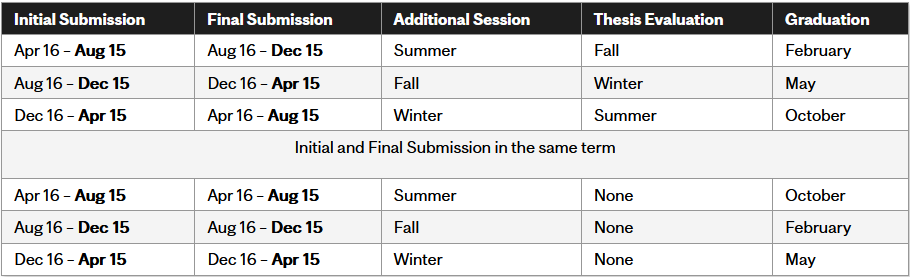
\includegraphics[width=0.9\linewidth]{Pictures/thesis_submission_deadlines.png}
        \label{fig:thesis_submission_deadlines}
    \end{figure}


    \begin{plaincorollary}
        The term after you submit your initial thesis is referred to as your thesis evaluation term which reduces the amount of tuition that you have to pay. For example: if you submit your thesis at the end of April, the summer term will count as your thesis evaluation term. You would need to make your final submission before the end of August if you wish to graduate in October.
    \end{plaincorollary}

    \subsection*{MSc Timeline}
    Here's a sample timeline for students starting their MSc program in Fall. You need not follow this exact roadmap. Use \href{https://horizon.mcgill.ca/myprogress/ResponsiveDashboard/}{myProgress} for a more comprehensive timeline and refer to \href{https://www.physics.mcgill.ca/grads/courses.html}{this} website for complete coursework requirements. The course credits are mentioned in the parenthesis.

    \begin{vtimeline}[description={text width=12cm}, row sep=2ex]
        Sem 1 & PHYS 601 (3) + PHYS 693 (3) + 2 Courses (3+3) \endlr 
        Sem 2 & PHYS 602 (3) + 2 Courses (3+3)\endlr
        Sem 3 & PHYS 690D1 (12) + 1 Course (3) \endlr
        Sem 4 & PHYS 690D2 (12) + Initial Thesis Submission\endlr
        Summer & Final Thesis Submission \endlr
    \end{vtimeline}

    If you join the program in the winter, you can do PHYS 602 in your first semester and then PHYS 601 in your second. These two courses can be taken in any order but they must be taken in consecutive terms. The research courses 690 and 693 remain in progress on your transcript untill you are granted a degree by the senate.
    
    It is recommended to take as many complementary courses in your first year so that you have more available time to focus on your thesis in your second year.

    \subsection{Fast-Tracking} \index{Fast-Tracking}
        On the recommendation of the Departmental Graduate Committee, fast-tracking from the M.Sc. program into the Ph.D. program may be granted after one year, if:  the student has fulfilled the M.Sc. coursework requirements, or;
        the candidate's Supervisor determines that the student qualifies based on the student's academic and research record.

        It is recommended to talk to your supervisor about fast-tracking! It has pros and cons, so please chat with your peers/supervisor to see if this is the best option for you.

        \textbf{If you do end up fast-tracking}, you will be a ``\textbf{PhD1}'' in your first year, which means that you will \textit{need} to register for the following courses: PHYS 715 PhD1 Research Credit Course 1 and PHYS 716 PhD1 Research Credit Course 2. These will be taken consecutively in your first year. 
    
    \subsection{PhD Requirements} \index{PhD Requirements}

    Complete details of degree requirements can be found \href{https://www.physics.mcgill.ca/grads/requirements.html}{here}. Candidates starting their PhD directly from a Bachelor's degree in Physics are referred to as ``\textbf{PhD1}''. Candidates entering their PhD program with an MSc degree in Physics or equivalent qualification are referred to as ``\textbf{PhD2}''.

     PhD1 students are required to take 30 research credits (PHYS 715 and PHYS 716) upon entry to the program. And they must complete 6 3-credit graduate courses at the 500 or 600 level or above, with at least three being at the 600 level. 
     
     PhD2 students need to do 2 3-credit graduate courses at the 600 level or above. One of the courses can be substituted if the student completed his MSc at McGill. 
    
    \subsubsection{Courses}
    
    Official course recommendations can be found \href{https://www.physics.mcgill.ca/grads/courses.html}{here}. Note that the department lists recommended courses according to your area of study. You do NOT \textit{need} to follow this recommendation, as long as you and your supervisor agree on which courses you should take based on your interest/research. You are also more than welcome to take courses outside the department/university, see the next section for more information. Students who did their undergrad at McGill may transfer 1 course for graduate credit if they did not need it to complete their undergraduate degree.

    \subsubsection{Letter of Understanding} \index{Letter of Understanding}

    The letter of understanding (LOU) is a way for you and your supervisor to be on the same page in terms of your research objectives, goals, and timeline. This is meant to be structured as a conversation and helps with communication and transparency. 

    Details on the generating this letter of understanding can be found \href{https://www.physics.mcgill.ca/grads/lou22.pdf}{here}.

    \subsubsection{Supervisory Committee}

    Your supervisory committee is a group of 3 professors (including your supervisor) meant to serve as your guides throughout the course of your PhD (think of it as an Order of Jedi to your young Padawan self). A meeting with your supervisory committee will be a yearly checkpoint to see how your research is progressing.

    For these checkpoints, you need to fill out the \href{https://www.mcgill.ca/gps/students/progress-tracking}{Graduate Student Progress Tracking Form} and submit it to GPS. 
    
    \subsubsection{Prelim} \index{Prelim}

    The prelim should be taken within 2.5 years of your program start date for PhD 1 students and within 1.5 years for PhD 2 students. This exam is aimed at testing undergraduate physics knowledge related to your research project, along with your understanding of your research problem and subfield. It has two components:
    \begin{itemize}
        \item A 10-page research proposal 
        \item An oral exam, which includes a 20 minute presentation and a 1-1.5hr question period.
    \end{itemize}

    The prelim committee consists of 4 people: your supervisory committee plus one prelim chair (a professor from a different research area).

    A lot more information about prelims (and in much more detail) can be found \href{https://www.physics.mcgill.ca/grads/prelim-candidate.html}{here}.

    In case of failure on your first try, you are allowed one final second attempt.

    Students who have taken the prelim in the past few years recommend confirming your prelim committee at least 2.5 months before the date of the exam. Usually, the availability of professors acts as the biggest obstacle. Since December is usually a busy time, if you can, try scheduling your prelim for end of November (this is not compulsory, just a suggestion; a lot of people still do prelims in December). It is also worth asking your supervisor which professors might be the best fit for your committee. 
    
    Although generally advertised as testing undergraduate knowledge, the latter part of the oral exam may involve questions about your research and your knowledge of the field. Expect to be challenged with hard questions -- most people find it to be so and it is not a reflection of how your exam is going. Professors may progressively ask harder questions to help you structure the direction of your research.

    \subsubsection{Thesis} \index{Thesis}

    All details for writing/submitting a thesis can be found \href{https://www.mcgill.ca/gps/thesis}{here}. 

    \subsection*{PhD Timeline}
    Here's a sample timeline for students starting at the PhD2 level in Fall. You need not follow this exact roadmap. Use \href{https://horizon.mcgill.ca/myprogress/ResponsiveDashboard/}{myProgress} for a more comprehensive timeline and refer to \href{https://www.physics.mcgill.ca/grads/courses.html}{this} website for complete coursework requirements. The course credits are mentioned in the parenthesis.

    \begin{vtimeline}[description={text width=14cm}, row sep=2ex]
        Sem 1 & PHYS 601 (3) + PhD2 Progress Tracking + 1 or 2 Courses (3+3) + LOU \endlr 
        Sem 2 & PHYS 602 (3) \endlr
        Summer & Prelim Prep (Report) \endlr
        Sem 3 & PHYS 700 (Prelim) =  PhD3 Progress Tracking \endlr
        Sem 4 &  \endlr
        Sem 5 &  PhD4 Progress Tracking \endlr
        Sem 6 & Individual Development Plan (IDP)  \endlr
        Sem 7 & PhD5 Progress Tracking\endlr
        Sem 8 & Initial Thesis Submission \endlr
        Summer & Final Thesis Submission \endlr
    \end{vtimeline}

    \section{Taking courses in a different department/university}\index{Courses outside McGill}
        It is entirely possible to take a course in a different department/university and still get credited for your degree. Note that although the physics department website outlines the courses that you \textit{should} be taking, it is entirely up to you and your supervisor to decide which courses will most benefit you and your research. This section will focus on the different ways in which you can take a course outside of the McGill physics department. 

        \subsection{Courses outside the Department Area}

        Depending on your research area, it might be wise to take a course outside of the physics department, such as, but not limited to, in the chemistry, engineering, and biology departments.

        Some supervisors encourage students to think as broadly as possible when planning their courses, which may involve taking more than the two out-of-department courses technically allowed for MSc and direct-entry PhD students. As long as the courses are relevant to your research area and you justify this to the GPC, this rule is quite flexible in practice. 

        \subsection{Courses outside the University}

There will be opportunities, often sent via email, to take courses at a different university. Many universities also offer courses to students in different institutions without publicising them. If you find that McGill does not offer enough relevant courses to fulfil program requirements, you might want to check the other universities in Québec or even Canada.

\subsubsection{Québec Universities}

The process for Québec universities is pretty simple, and McGill has a \href{https://www.mcgill.ca/transfercredit/iut}{page specifically for it}:
\begin{enumerate}
    \item Go on the \href{https://aehe.bci-qc.ca/en}{AEHE portal}.
    \item Click on "Applications" and select McGill as your home institution.
    \item Log in with your McGill student account.
    \item Accept the terms of use and click "Submit".
    \item Accept the information transfer description. Change the frequency of verification if desired.
    \item Select "Student" as your occupation.
    \item Agree to the terms and conditions again.
    \item Click on "New Application"
    \item Log in with your McGill credentials (if not automatically redirected to the log-in window, click on Azure SSO)
    \item Verify that the information provided is correct
    \item Select the correct program is not already selected
    \item Select the appropriate semester and click on "Create Request"
    \item Add your desired class by looking up the host university and location
    \item Add the desired class by double-clicking it and filling out the information. 
    \begin{itemize}
        \item The schedule and section are only truly relevant when the same class is offered in multiple instances, but you should fill it out nonetheless
        \item Try to find the closest equivalent at McGill to add in the replacement section
        \item In the comments, briefly describe why you are taking a class outside McGill
    \end{itemize} 
    \item Once you have added the desired course, you can submit the application.
\end{enumerate}
It might take a while to hear back from the host university. It is recommended that you stay in contact with the prof directly so that you can be updated on the course start date and the first few assignments and documents in case you do not have access to the host university's website in time. 

\subsubsection{Other Canadian Universities}
The exact process varies across universities. General advice from people who took a class at another university: contact the graduate coordinator for the physics program at the host university directly. They will send you the relevant forms. This should be done as soon as possible as the process can be long and arduous. 

In addition, for courses outside McGill (both in Québec and outside Québec), the course grades cannot be transferred. This means that these course grades will be pass/fail (or Satisfactory/Unsatisfactory in McGill terminology) and you will only get the credit but it will not count towards your GPA. Students must also make sure that the courses are offered by an institution in some sort of graduate exchange agreement (e.g. these is one between McGill, UBC, UdeM, and UToronto). Through these exchange agreements, students do not pay tuition to the school at which they are taking a course. Students must provide official syllabi for the courses (which cannot be a PDF of the course website according to the Faculty of Sciences) and then pay to officially send the transcript from said school to McGill after the term ends. 


     
        
\chapterimage{health.pdf}
\chapterimagecaption{\textit{Lunch atop a Skyscraper (1932)} by Charles Clyde Ebbets?}

\chapter{Health and Safety}

    \section{Health Insurance} \index{Health Insurance}
    
\subsection{Canadian Students}

\subsubsection{PGSS Health Insurance}
    Canadian Graduate students are offered Health and Dental plans by PGSS. The billing for these is included in your student fees. The plans are separate, you can choose either one or the other, both of them, or neither. They include coverage on:
    \begin{itemize}
        \item Health (prescription drugs, vaccinations, discounts on physio, massage, chiro, etc.)
        \item Vision (glasses, some eye exams/surgery)
        \item Travel (insurance for travel health, cancellation, etc.)
        \item Dental (covers most cleanings, oral surgery, etc.)
        \item Gender Affirmation Care (certain surgeries and other treatments)
    \end{itemize}

    There is an additional Legal Care Program for \$50 per year (also automatically opted in, billed in student fees). Note that there is different coverage based on whether you take the \textbf{Basic} or \textbf{Enhanced} Care Plan. Cost breakdown can be found \href{https://studentcare.ca/rte/en/McGillUniversitygraduatestudentsPGSS_Cost_HowMuchDoesItCost}{here}.
    \textbf{Keep in mind that students are \textit{automatically} enrolled in ENHANCED Health and Dental Plans!} What can you do in this case?
    \begin{itemize}
        \item Keep the Enhanced plans
        \item Change to Basic plans (you can pick and choose whether you want both Health and Dental to be Basic, or just choose one of them as Basic and the other Enhanced)*
        \item Opt-out of the Health and Dental Plans entirely*
        \item Modify your plan to add family members*
    \end{itemize}

    *For these changes, you MUST do this before the Opt-Out/Changes deadline every semester, which is usually close to the end of September for Fall incoming students, and close to the end of January for Winter incoming students. More details on Opt-outs/changes can be found \href{https://www.studentcare.ca/rte/en/McGillUniversitygraduatestudentsPGSS_ChangeofCoverage_OptOuts}{here}.
    
    Extensive detail surrounding the coverage can be found on PGSS's \href{https://studentcare.ca/rte/en/McGillUniversitygraduatestudentsPGSS_Home}{Studentcare website}. If you want a quick overview, please see this \href{https://pgss.mcgill.ca/document/view/10773/PGSS%20Studentcare%20Health%20and%20Dental%20Insurance%20Presentation.pdf}{document}.

    \subsubsection{Provincial Health Insurance} \index{Health Insurance! Provincial Health Insurance}
    If you are a Canadian from outside of Québec who only came to Montréal to pursue your studies, you are considered a temporary resident in Québec and therefore are not eligible to obtain RAMQ (Régie de l'assurance maladie du Québec). You can be covered by RAMQ if you decide to settle in Québec, please consult \href{https://www.ramq.gouv.qc.ca/en/citizens/health-insurance/register}{the official eligibility check}. \index{Health Insurance!RAMQ}

    If you wish, you can register for RAMQ through this \href{https://www.ramq.gouv.qc.ca/en/citizens/health-insurance/registration-information}{application}. However, it should be noted that anyone aged 26 or older will be required to pay for the Public Prescription Drug Insurance Plan if they do not have access to a private plan. Relevantly, the PGSS Health Insurance is NOT considered a private plan for this purpose. As of Aug 2026, its \href{https://www.ramq.gouv.qc.ca/en/citizens/prescription-drug-insurance/annual-premium}{annual rate} is \$789 per person.
    
    Canadian students from another province can remain covered under their province or territory of origin by virtue of the interprovincial health insurance agreements concluded between the Canadian provinces and territories. To maintain your coverage, you will need to notify your home province of your absences for full-time study purposes. Find the applicable procedure for your home province in \href{https://pgss.mcgill.ca/en/ramq-_-provincial-health-insurance}{this list}. Furthermore, you will need to file taxes in your home province instead of in Québec (see \hyperref[tax]{\textcolor{purble}{\ref*{tax}}}).

    For out-of-province Canadian students, appointments at the McGill's Wellness Hub tend to be the most hassle free as they handle all the insurances behind the scene for you. For off-campus resources, you will have to pay upfront for an appointment, but can submit the receipts to your home province for reimbursements. However, if approved, you are reimbursed according to your province's standard medical fee rates, which may not cover the full amount you were charged in Québec. The difference may then be submitted for reimbursements to the PGSS Health Insurance.

    Canadian non-residents who came here to study have to obtain the International Health Insurance until they have established residency in Canada. These are more specific cases and we encourage students in such situation to reach out directly to \href{https://www.mcgill.ca/student-accounts/tuition-fees/non-tuition-charges/insurance}{McGill Student Services} for help.
    
\subsection{International Students}

    Please refer to Section  
\hyperref[section:inthealth]{\textcolor{purble}{\ref*{section:inthealth}}}
    for more health insurance details specifically applying to international students. The \href{https://www.mcgill.ca/internationalstudents/health/benefits/handbook}{IHI handbook} details exact coverage amounts for each type of health service. 
    
\section{Health Resources}

    \subsection{Physical Health}

    For \textbf{on-campus care}, the \href{https://www.mcgill.ca/wellness-hub/}{Wellness Hub} offers a wide range of services. To meet with a nurse/doctor/counsellor, you can follow \href{https://www.mcgill.ca/wellness-hub/contact}{these instructions} to book an appointment.

    \begin{plaincorollary}
    Appointments with a physician at the Wellness Hub cannot be booked more than a day in advance. Same-day appointments go quickly. You need to call exactly at the opening time to secure a spot. Once on the line, keep pressing 1 instead of waiting for all the prompts.
    \end{plaincorollary}

    For \textbf{off-campus} care, please visit \href{https://www.mcgill.ca/wellness-hub/get-support/find-community-resources/navigatinghealthcare}{this website}, which provides a list of off-campus clinics and healthcare providers. 

    We also get \textbf{Virtual Care}! Our virtual care is through Maple, which provides an easy way to virtually consult physicians on the same day. Depending on the issue, you can get prescribed medication through Maple. More information on Maple and creating an account can be found \href{https://www.mcgill.ca/internationalstudents/health/benefits/maple-virtual-care}{here}.
    

    \subsection{Mental Health}
    For mental health resources, visit the 
    \href{https://www.mcgill.ca/wellness-hub/get-support/mental-health-support}{McGill Wellness Hub}. You can also talk to a licensed-therapist via Maple included in your health insurance. PGSS also provides a list of resources \href{https://pgss.mcgill.ca/en/mental-health-resources}{here} and the physics department has a list of emergency contacts \href{https://www.physics.mcgill.ca/resources/grads.html}{here}. 
    

    \section{How to File Complaints} \index{Complaints}
    

\subsection{Building Complaints}

If you have any issues with the building, you can address your concern to any of the following individuals:
\begin{itemize}
  \item MGAPS Workspace and Accessibility Officer
  \item Physics Building Director: \href{mailto:buildingdirector.physics@mcgill.ca}{buildingdirector.physics@mcgill.ca} (currently Andreas Warburton)
\end{itemize}

\subsection{Safety Complaints}\index{Safety}

For any \textbf{campus safety concerns}, you can:
\begin{itemize}
    \item Call campus security (514-398-3000) or 911. \textbf{These numbers are in case of emergencies}
    \item Call campus security for general inquiries (514-398-4556)
    \item Learn more about campus public safety \href{https://www.mcgill.ca/campussafety/}{here}.
\end{itemize} 

In case of sexual violence/assault, or in case of witnessing sexual violence/assault, you can use these following resources. These resources are meant to be \textbf{entirely confidential}.
\begin{itemize}
    \item Sexual Assault Center of the McGill Students Society (SACOMSS) \href{www.sacomss.org}{www.sacomss.org}
    \item Office for Sexual Violence Response, Support and Education (OVRSE) \href{https://www.mcgill.ca/osvrse/}{www.mcgill.ca/osvrse}
\end{itemize}

\subsection{Supervisor Complaints}

If you have issues with your supervisor that cannot be resolved between you and your supervisor, you next person to contact would be the Graduate Program Director (GPD), who is currently Nik Provatas.
If this is still not working, please visit \href{https://www.mcgill.ca/expmed/policies/conflict-resolution-policy}{this website} for more details on who to contact/how to navigate the hierarchy of help. This is also expanded on in Section \hyperref[section:supercomp]{\textcolor{purble}{\ref*{section:supercomp}}}.


\chapterimage{finance.pdf}
\chapterimagecaption{\textit{At the Roulette Table in Monte Carlo} (1892) by Edvard Munch}

\chapter{Financial Information} \index{Finances}


    \section{Travel Guidelines} \index{Travel}
    When travelling on behalf of McGill there are four main things to arrange, depending on your specific circumstances: \textbf{Travel insurance, accommodation, transport, food, and visas}.    \href{https://www.mcgill.ca/financialservices/policies/reimburse/procedures}{\textbf{Read through this website first before proceeding.}}

     The aim of this section is to give a brief outline of the process as well as provide some information on grants and awards to fund your travel.


  \subsection{Travel Insurance} \index{Travel! Insurance}
    Travel insurance is essential so that you're covered for any emergency medical expenses abroad. The insurance is provided through PGSS or McGill at no additional cost.
    
    \begin{itemize}
    \item Canadian Citizens (anyone that accesses PGSS Health plan):\\
    Coverage provided by PGSS, see this \href{https://studentcare.ca/rte/en/McGilluniversitygraduatestudentspgss\_Travel\_TravelCoverage}{site}.\vspace{5pt}

    \item International Students:\\
    Coverage provided through \href{https://www.mcgill.ca/internationalstudents/health/benefits/going-abroad}{extension} of Blue Cross International Health Insurance (up to 4 weeks).
    \end{itemize}

    \subsection{Accomodation} \index{Travel! Accomodation}
    \begin{itemize}
    \item Before booking anywhere to stay, first determine if your conference/event provides any funding for accommodation (many do!). If this is the case, there will likely be a per night price limit up to which they will reimburse, as well as a restriction on how many nights before/after the scheduled programming they will support. For example, if the conference runs Monday to Friday, they most likely will fund Sunday night to Friday night inclusive.
    \item If the event will not provide any lodging support, speak with your supervisor to determine if they will support your stay. Most groups in the physics department will fund their student’s accommodation.
    \item If your accommodation is covered (either by your supervisor’s grant funds or by the conference hosts), it will likely be in the form of a reimbursement after the event. It is therefore recommended to look for accommodation that only requires you to pay the full amount nearer/upon check in, so that the money is not tied up for months on end.
    \item To be reimbursed with your supervisor’s grant funds, you should follow the guide below on reimbursements (section \hyperref[section:reimbursement]{\textcolor{purble}{\ref*{section:reimbursement}}}).
    \item The process to obtain reimbursement from the event organizers will vary depending on the host institution. However, most events will have dedicated in house organization/admin staff to assist with this process.
    \item Many conferences will provide hotel recommendations upon registration, so be sure to look out for these!\\

    \end{itemize}


    \subsection{Transport} \index{Travel! Transport}

    \noindent If you need to take a flight, there are two main ways to approach booking and paying for it:
    \begin{enumerate}
        \item Direct billing of your supervisor’s grant fund
        \item You pay (and then are possibly reimbursed)
    \end{enumerate}

    \noindent The first method is recommended, so you are not out of pocket for the months leading up to the event. If you're going to take a train/coach/anything else, this option is not available, so you must book with your own money and then seek reimbursement (see section \hyperref[section:reimbursement]{\textcolor{purble}{\ref*{section:reimbursement}}}).\\

    \subsection*{Guide for direct billing method}  
    (Read in it’s entirety before proceeding)\\

    \begin{itemize}[leftmargin=10pt]
        \item Go to \url{https://www.mcgill.ca/travelservices/transport/tmc} and click ‘Create New Profile’. Enter your details, then wait for the account to be approved by admin staff. Then log in by clicking ‘Access Existing Profile’.
        \begin{figure}[H]
            \centering
            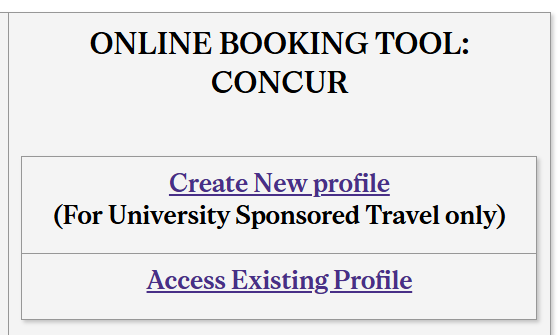
\includegraphics[width=0.4\columnwidth]{Pictures/CreateAccount.png}
        \end{figure}

        \item Navigate to the flight tab, and read the provided instructions for an overview of the process. Note that the Workday step at the end is only available from September to April. Over the summer, this step can be completed by submitting a ticket to the Finance Service Desk (\url{https://hrservicedesk.mcgill.ca/servicedesk/customer/portal/12}), under the category ‘WE-Airfare/Rail (Spend Authorization’. 

        \begin{figure}[H]
            \centering
            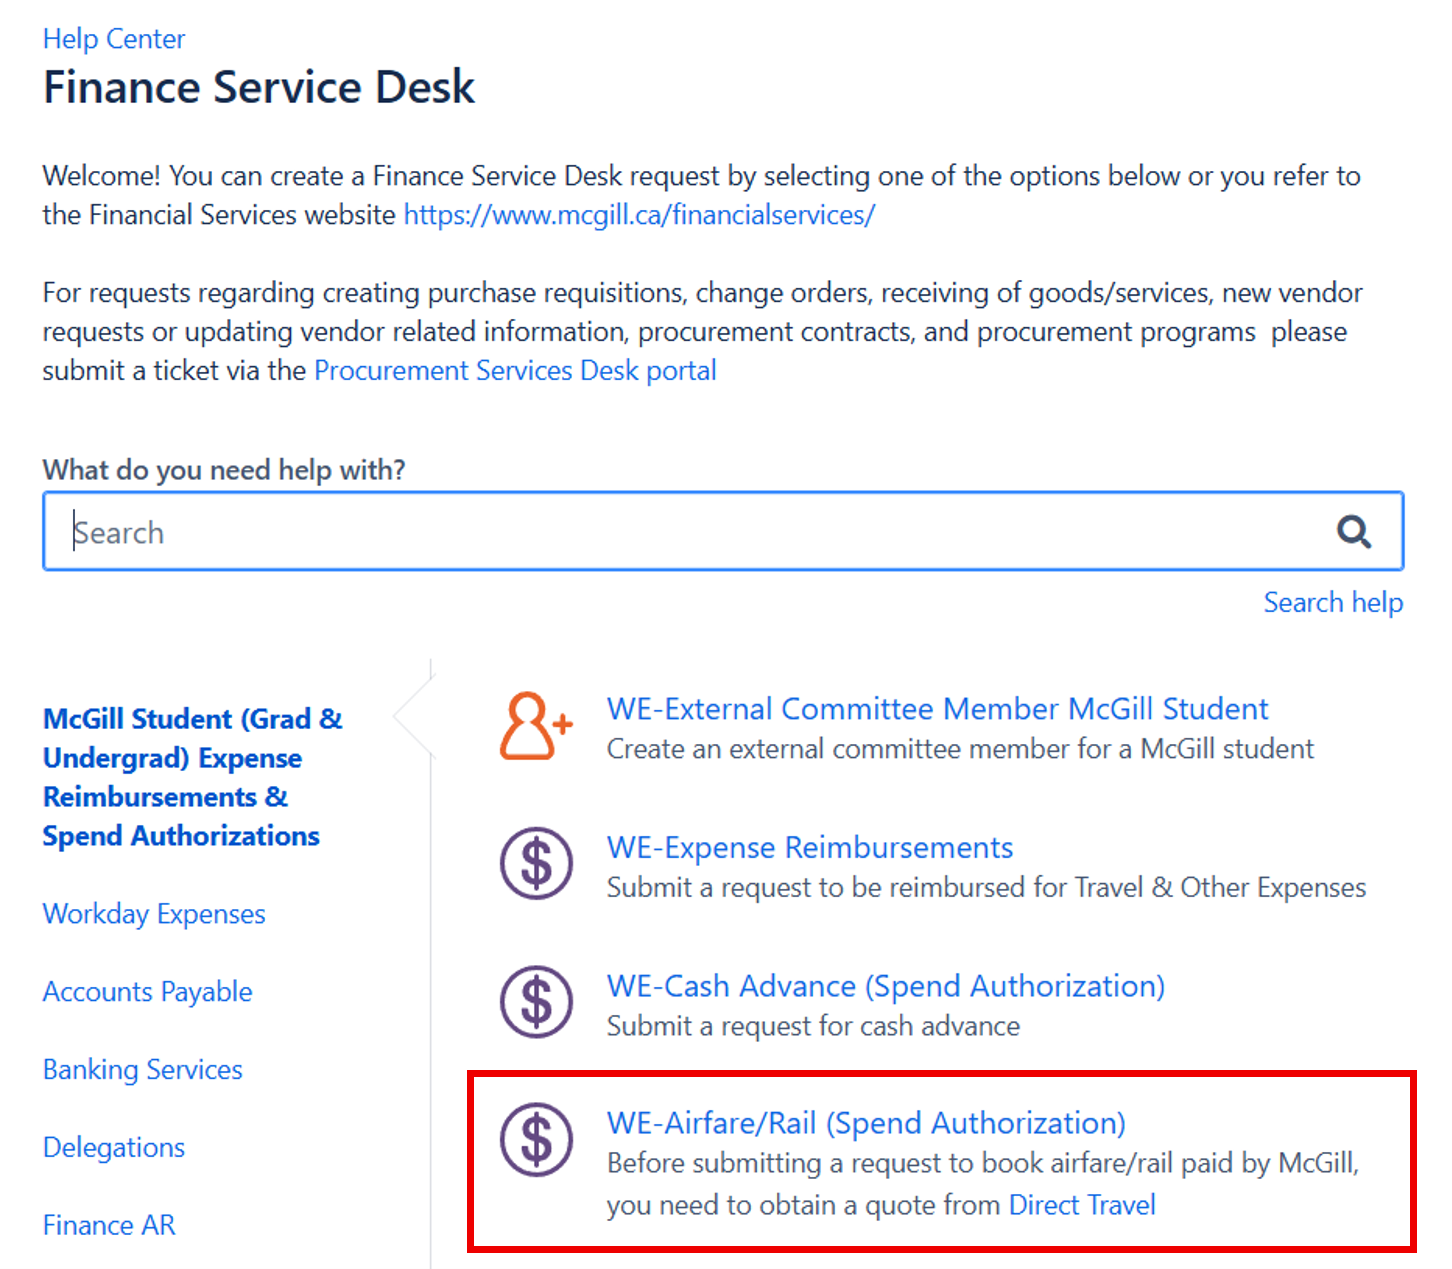
\includegraphics[width=0.65\columnwidth]{Pictures/SpendAuth.png}
        \end{figure}

        \item \textbf{\color{ocre}Important:} This approval can only be processed during regular business hours (Mon - Fri 08:30 - 17:00). The flight can only be held for 24 hours, so it is recommended that you only proceed from here between Monday morning and Friday morning, and account for any public holidays.\\

        \item Use the search tool to find appropriate flights. Find the cheapest flights that don’t have a ridiculous layover, or your supervisor may refuse to pay (i.e. no business class). You should take screenshot proof that you have selected a low cost flight relative to equivalents. Be sure to get this when booking. Also be sure to check the baggage and cancellation policy of any flights, and pick what is most suitable for your situation. Select your desired flights. \\

        \item On the ‘Review and Book’ screen, input your traveler information, and reserve seats if desired. In the ‘Form of Payment’ drop down menu, select ‘Spend Authorization’.
        
        \begin{figure}[H]
            \centering
            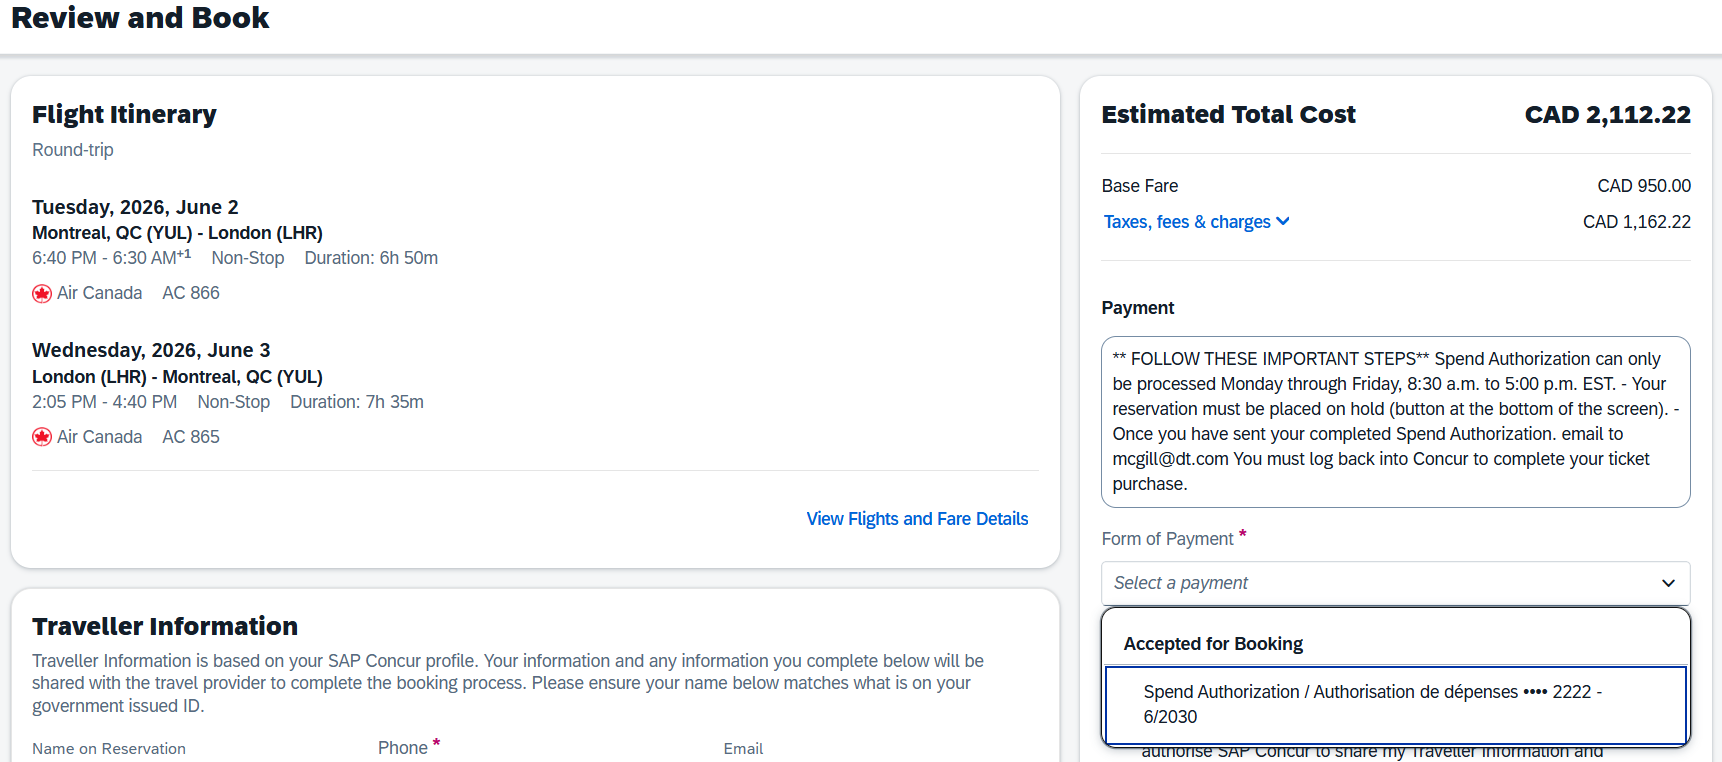
\includegraphics[width=0.7\columnwidth]{Pictures/DropDownMenu.png}
        \end{figure}

        \item Now press ‘Book and Continue’. Note that this does NOT finalize the trip yet. On the next screen, press ‘Hold Trip’. \\
        
        \item You now have 24 hours to have the spend authorization approved by the Finance Service Desk and your supervisor/whoever is paying. To do this, either submit on Workday under the spend authorization section (September – April), or via the Finance Service Desk Jira tool via the link above (May – August). When doing so, you will need to provide evidence of your booking and the cost breakdown. For this, use the flight hold confirmation email you should have received, as well as the screenshot proving your flight was the cheapest option, taken earlier. You will also need your supervisor’s 6 digit research fund code so the spend authorization is charged to the correct account. When approved, you will receive a 7 digit ‘Spend Authorization Number’ that you can input on the final screen. Input this, and then click ‘Finalize Trip’. Your flights are now confirmed. \\

        \begin{figure}[H]
            \centering
            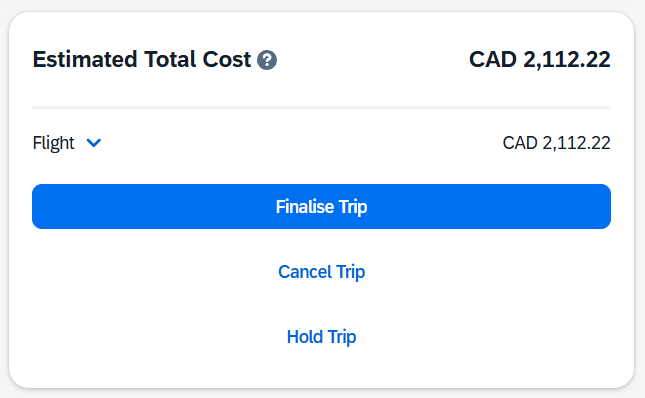
\includegraphics[width=0.5\columnwidth]{Pictures/Finalise.png}
        \end{figure}
        
    \end{itemize}

    \subsection*{Booking flights yourself}
    You would often prefer booking flights yourself, especially if you wish to travel outside of work and spend time visiting places before and after the conference/workshop. The process may seem tiring but it's often the simplest way to book tickets. 
    
    When booking flights on your own, you must provide a \textbf{travel quote} for the event $\pm$ 1 days. Withing \textbf{24 hours} of booking a flight, you need to go to your favourite flight search website such as \href{https://www.skyscanner.ca/}{Skyscanner} or \href{https://www.expedia.ca/Flights}{Expedia} and print the page (Ctrl + P) for travel dates corresponding to the \textbf{\textit{actual dates}} of the conference. The date and time you took the screenshot should be clearly visible at the top. You just need to provide around 10-15 options with various combinations to show that you picked the cheapest option. 
    
    Here's an example that should solve all your queries. 

    \begin{plaincorollary}
    Bob wants to attend a conference in Geneva from $10^{\rm th}-15^{\rm th}$ July. He plans to arrive a day early on the $9^{\rm th}$, so he leaves Montr\'eal on the $8^{\rm th}$. He plans to stay and visit some places in France after the conference and catch a flight back to Montr\'eal from Paris on the $20^{\rm th}$. 

    He books a flight Montr\'eal $\rightarrow$ Geneva on the $8^{\rm th}$ (arriving $9^{\rm th}$) and a return flight from Paris $\rightarrow$ Montr\'eal on the $20^{\rm th}$. This includes his ``leisure'' travel. Suppose this multicity flight costed him \$X. He must also provide a roundtrip airfare \textbf{quote} from $8^{\rm th}$ to $16^{\rm th}$ (one day before and after the conference) from Montr\'eal $\rightarrow$ Geneva. Say this costs \$Y. This is his ``work-related'' travel cost. He will be reimbursed the lower of X \& Y.     
    
    Preferably, he should also provide a quote using other combinations of dates such as $8^{\rm th}$ to $17^{\rm th}$ from Montr\'eal to other surrounding airports like Lyon to avoid the fury of the financial desk. In summary, a travel quote illustrates \textbf{hypothetical work-related expense} and is the maximum he will be reimbursed for.    
    \end{plaincorollary}

    \begin{figure*}[hbt]
        \centering
        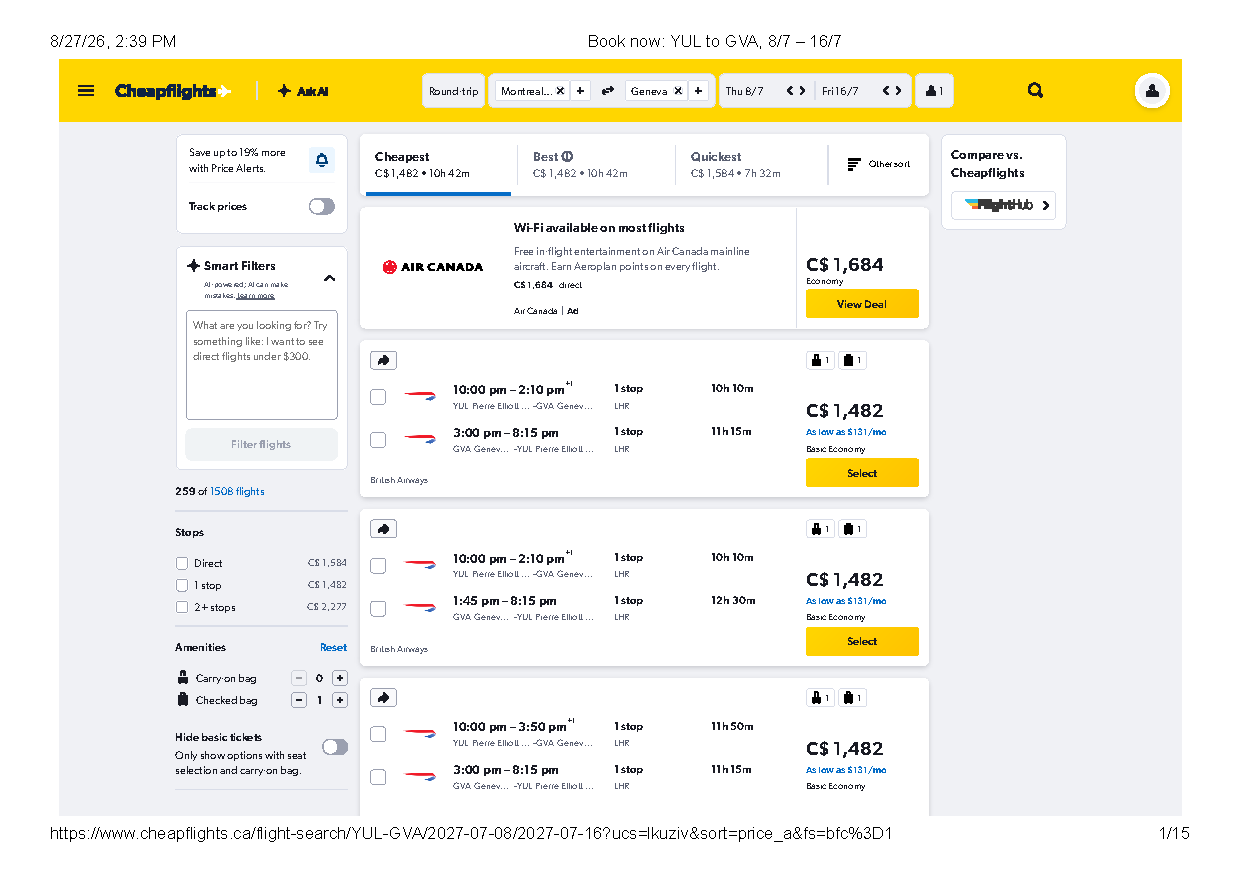
\includegraphics[width=\linewidth]{Pictures/quote.pdf}
        \caption*{A sample travel quote from Montr\'eal to Geneva from $8^{\rm th}$ to $16^{\rm th}$ July. The date and time is clearly visible at the top. The website name is visible at the bottom. The cheapest flight options don't usually include baggage, so checked baggage has been selected on the left.}
        \label{fig:quote}
    \end{figure*}


    \subsection{Food}
    You can either claim a per-diem or provide actual receipts. Usually, per-diems are preferable since the amount is usually higher than what you are expected to spend and also the travel desk doesn't have to scour through your receipts. You must discuss this with your supervisor before embarking on your odyssey. Current per-diem rates are given below (effective May $1^{\rm st}$ 2026). This is the \textbf{maximum} that you are allowed to spend per day on food.

    \vspace{-5 pt}
    \begin{table}[h!]
        \hspace*{-1.7cm}
    \centering
    \renewcommand{\arraystretch}{1.2}
    \arrayrulecolor{ocre}
    \begin{tabular}{|>{\columncolor{ocre!20}}lc|c|}
    \hline
    \rowcolor{ocre!60}
  {\color{white}\sffamily \textbf{Meal}} & {\color{white}\sffamily \textbf{Inside Canada}}  & {\color{white}\sffamily \textbf{Outside Canada}} \\
        Breakfast & \$24 & \$30 \\
        Lunch & \$30 & \$40\\
        Dinner & \$68 & \$81\\
        \hline
        Total & \$122 & \$151\\
        \hline
\end{tabular}
\arrayrulecolor{black}
\end{table}
When filing for reimbursement, you must attach a spreadsheet detailing the days of work travel and the eligible amount for each day. If breakfast is included in your hotel or if dinner is included in the conference reception, you may not be able to per-diem for that item. You can claim a per-diem $\pm 1$ day before and after the conference or workshop.
    
    \subsection{Visas} \index{Travel! Visa}
    MGAPS cannot provide direct visa advice given the diversities in nationalities of the student body as well as variance in the procedures from country to country. Generally, it is recommended that you do your own in depth research and leave plenty of time for any applications and interviews that may be required. If further assistance is required, be sure to contact either the Graduate Program Director (currently Nikolas Provatas, July 2026) or \href{https://www.mcgill.ca/internationalstudents/ihi-contact-us}{International Student Services}.


    \subsection{Travel funding opportunities} \index{Travel! Funding}
    Below is a list of travel awards to consider if you need additional funding for academic travel. Most are field specific, however some are generalized. This list will be continually expanded as we learn of more and more funding opportunities. If you know of any that aren't mentioned here, please get in touch so that we can add it.

   \subsubsection{General}

    \begin{enumerate}
        \item  PGSS Travel Award: \url{https://pgss.mcgill.ca/en/pgss-travel-grants}.
    \begin{itemize}
        \item Provides up to \$750 to cover travel costs.
        \item Award cycles every two months (6 per year).
        \item Can only be awarded once to a given student every TWO fiscal years.
        \item Need to submit letter of intent, letter of reference from faculty and a detailed budget (see website for template).
        \item For the budget, it is recommended that you put much more detail than is required. Justify every expense however small with ample evidence. For example, provide screenshots showing that your flights/accommodation are the cheapest available, or provide links to public transit websites showing fare prices.
        \item Ensure the budget is balanced (total costs and total funding match).\\
    \end{itemize}

    \item  McGill Graduate Mobility Awards (primarily for exchanges): 
    \begin{itemize}
    \item \url{https://www.mcgill.ca/gps/funding/travel}\\
    \end{itemize}

    \item  Physics Department Travel Award:
    \begin{itemize}
    \item \url{https://www.physics.mcgill.ca/grads/travel.html}
    \item \url{https://www.physics.mcgill.ca/grads/gtapp.pdf}
    \item \url{https://www.physics.mcgill.ca/cgi-bin/gta.pl}\\
    \end{itemize}
    
    \end{enumerate}
        
   
    \subsubsection{Nuclear/Particle/HEP}
    \begin{itemize}
        \item \url{https://cinp.ca/junior-scientist-travel-support-program-jsci}
        \item \url{https://cinp.ca/wnppc-graduate-student-travel-awards}
        \item \url{https://cinp.ca/cupc-student-travel-awards}
        \item \url{https://cinp.ca/conference-support}
        \item  \url{https://mcdonaldinstitute.ca/funding-opportunities-2/}
        \item \url{https://mcdonaldinstitute.ca/funding-opportunities/graduate-student-exchange/}
    \end{itemize} 

    \subsubsection{Medical Physics}
    \begin{itemize}
        \item \url{https://comp-ocpm.ca/awards/comp-idea-student-travel-grant}
    \end{itemize}

    \subsubsection{Condensed Matter/Materials/Biophysics}
    \begin{itemize}
        \item \url{https://rqmp.ca/en/call-for-applications/}
    \end{itemize}

    \subsubsection{Astrophysics}

    \begin{itemize}
        \item RADEATE grant. Sponsors 8 weeks of travel and fieldwork, if your supervisor is any of: Adrian Liu, Cynthia Chiang, Jon Sievers, Jason Hessels, Vicky Kaspi, Matt Dobbs + possibly some others (speak to Adrian).
        \item AstroQuébec/CRAQ. Wide breadth of funding opportunities, check \url{https://www.craq-astro.ca/le-craq/nos-programmes-de-bourses/} for updates.
    \end{itemize}

    \subsubsection{Other}
    \begin{enumerate}
        \item  Statistical Society of Canada: 
    \begin{itemize}
    \item \url{https://ssc.ca/en/sources-financement-pour-assister-a-congres}\\
    \end{itemize}
    \end{enumerate}
  \vspace{-10pt}  
    
\subsection{General Links}
\begin{itemize}
   \item Checklist: \url{https://www.mcgill.ca/biology/files/biology/pod1\_expense\_report\_checklist.pdf} (outdated but include a lot of still pertinent information).
   \item Contacts: \href{mailto:sciencefinancepod1@mcgill.ca}{sciencefinancepod1@mcgill.ca}
   \item  Per diem spreadsheet 
        \begin{figure}[H]
        \centering
        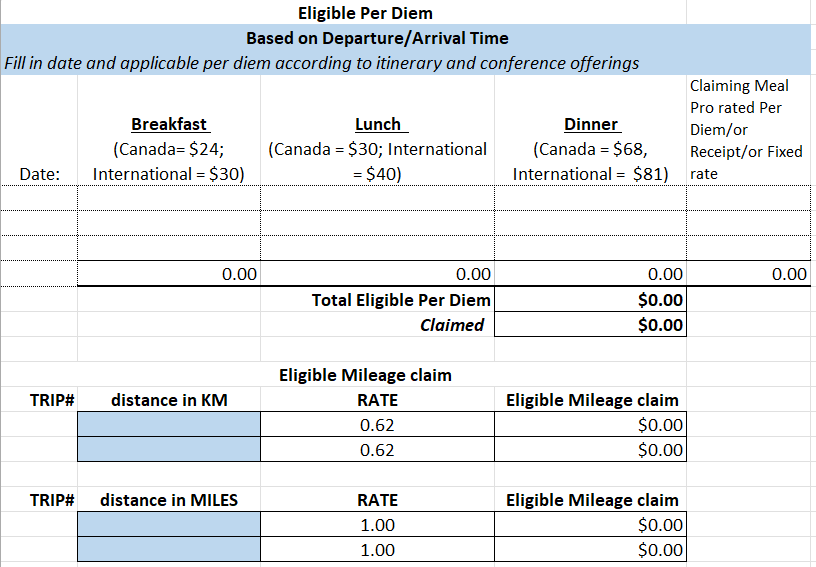
\includegraphics[width=0.7\columnwidth]{Pictures/per diem.png}
    \end{figure}
\end{itemize}

    \section{Reimbursements/Advances} \label{section:reimbursement}\index{Reimbursement} \index{Advance}
    

    \noindent The following section will outline the process of obtaining reimbursement for work-related expenses or conference travel. Most likely, you will need to spend your own money first and then have it reimbursed. It is also possible to get cash advances under certain circumstances, to help offset the financial burden of paying upfront. However, they are only available up to \textbf{30 days} prior to the start of the trip, limiting their usefulness.

    \begin{plaincorollary}
    \noindent Both reimbursements and advances follow a similar procedure. Confusingly, this process changes depending on the time of year. During the regular school year (September to April inclusive), you will have access to the \textbf{\color{ocre} McGill Workday} website to submit the reimbursement/advance. But over the summer, access is annoyingly unavailable, so you must submit a \textbf{\color{ocre}Jira ticket} to the finance desk.
    \end{plaincorollary}
    
\subsection{Workday Reimbursement (Fall \& Winter)} \index{Reimbursement} \index{Workday}

A detailed guide on Workday reimbursement is available on this \href{https://general-knowledgebase.mcgill.ca/spaces/FSKB/pages/124292739/How+to+Create+an+Expense+Report}{\underline{\textbf{link}}}, which has been transcribed here for archival reasons.

\begin{enumerate}[leftmargin=10pt]
    \item Log in to \href{https://wd3.myworkday.com/mcgill/d/home.htmld}{Workday.}\\

    \item On the welcome page, select “Expense Hub”.
        \begin{figure}[H]
            \centering
            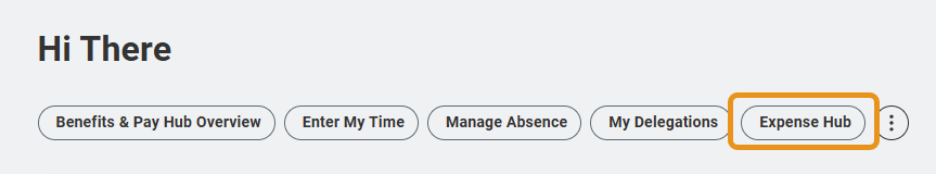
\includegraphics[width=0.8\columnwidth]{Pictures/ExpenseHub.png}
    \end{figure}

    \item Email ingestion information will display. Email ingestion allows employees to upload their receipts directly to their Workday Expenses profile, via a specific email address. Optical Character Recognition (OCR) can accurately read and interpret receipt data to automatically create quick expenses that can be easily added to expense reports. 

    \begin{figure}[H]
            \centering
            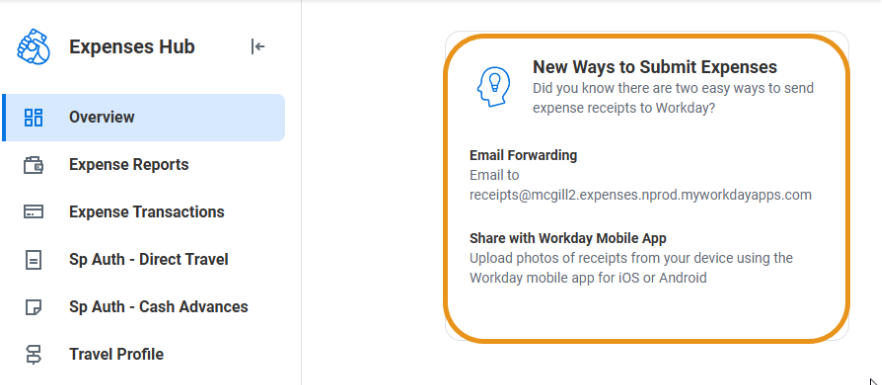
\includegraphics[width=0.8\columnwidth]{Pictures/EmailIngestion.png}
    \end{figure}

    \item Under ‘Tasks’, select “Create Expense Report”.

    \begin{figure}[H]
            \centering
            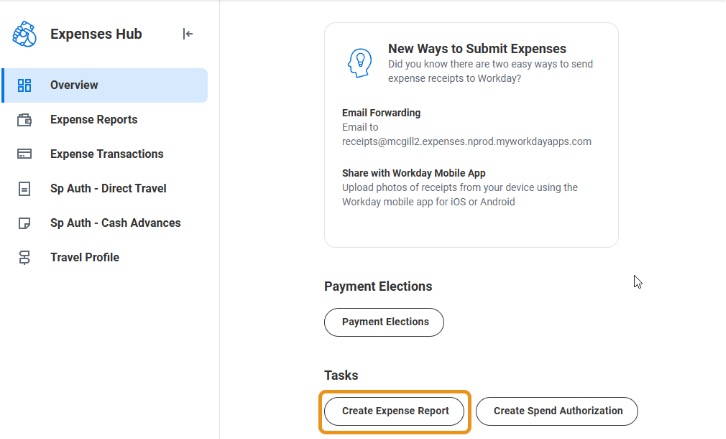
\includegraphics[width=0.8\columnwidth]{Pictures/CreateExpenseReport.png}
    \end{figure}

    \item In the newly opened page, select one of the following options: 
    
    \begin{figure}[H]
            \centering
            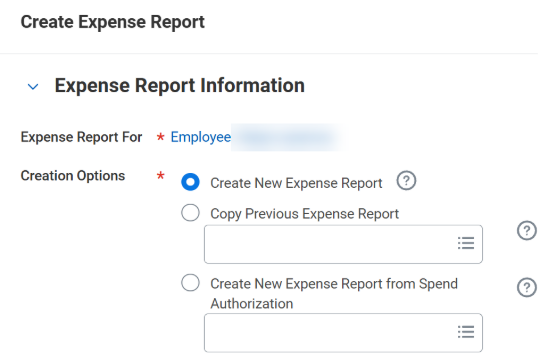
\includegraphics[width=0.5\columnwidth]{Pictures/ExpenseReportInformation.png}
    \end{figure}

    Select the correct option corresponding to your situation as described in the following table:

    \begin{figure}[H]
            \centering
            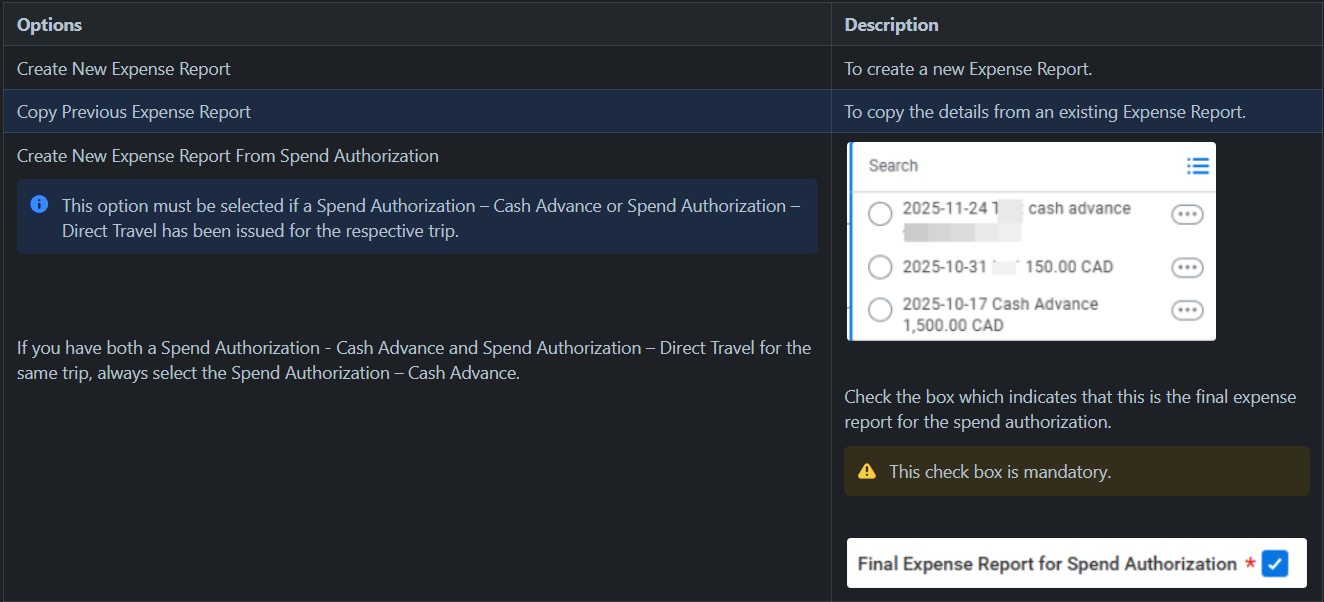
\includegraphics[width=0.8\columnwidth]{Pictures/NewExpenseReportTable.png}
    \end{figure}
    
    \item Continue completing the fields as listed below:

    \begin{figure}[H]
            \centering
            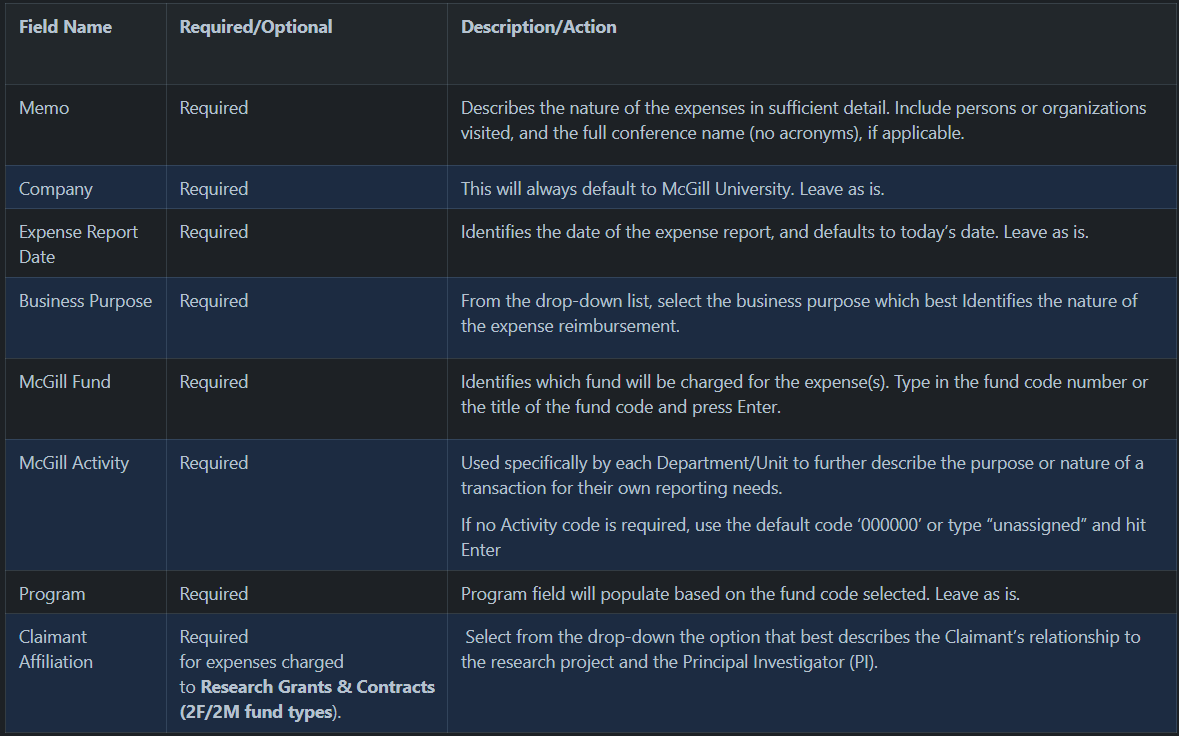
\includegraphics[width=0.8\columnwidth]{Pictures/FormFields.png}
    \end{figure}

    \item If this is the first time you complete an Expense Report for yourself, ensure the Enable Tax field is checked. This is used to calculate and report taxes accordingly. The system will not let you proceed without having this box checked.  All subsequent Expense Reports will automatically have this box checked.\\

    \item If you have uploaded receipts to your profile through email ingestion or the Workday mobile app, they will appear under Quick Expenses. Any expenses charged to a company credit card (i.e. Direct Travel) will appear as credit card transactions. Check off which quick expenses and/or credit card transactions are to be included in the expense report, if applicable.
    
    \begin{figure}[H]
            \centering
        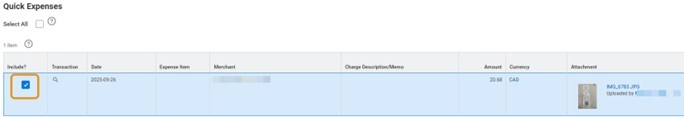
\includegraphics[width=0.9\columnwidth]{Pictures/QuickExpenses.jpg}
    \end{figure}

    \item If no quick expenses or credit card transactions are to be included in the expense report, proceed to step 10.\\

    \item Once this first page is complete, click \textbf{OK}. The information entered will serve as the Header of the Expense Report.\\

    \item   A unique expense report number will be generated, EXP-00000XX. The name of the employee will also display, as well as the status of the Expense Report, if any cash advance is applied, amounts previously paid by the university (i.e: to Direct Travel) and the reimbursable amount. These last fields will automatically update as expense items are added.\\

    \item The next step is to click ‘Add’ to add new expense lines. You can also add additional quick expenses or credit card transactions if available/uploaded in your profile.\\

   \item If you are adding a new expense, proceed to step 14. If quick expenses were included from the header page, separate expense line items will be created for each and will populate some of the information from the receipt, along with the receipt(s) as attachment(s). Complete the remaining fields as listed in step 16.\\

   \item The following page will display:

    \begin{figure}[H]
            \centering
            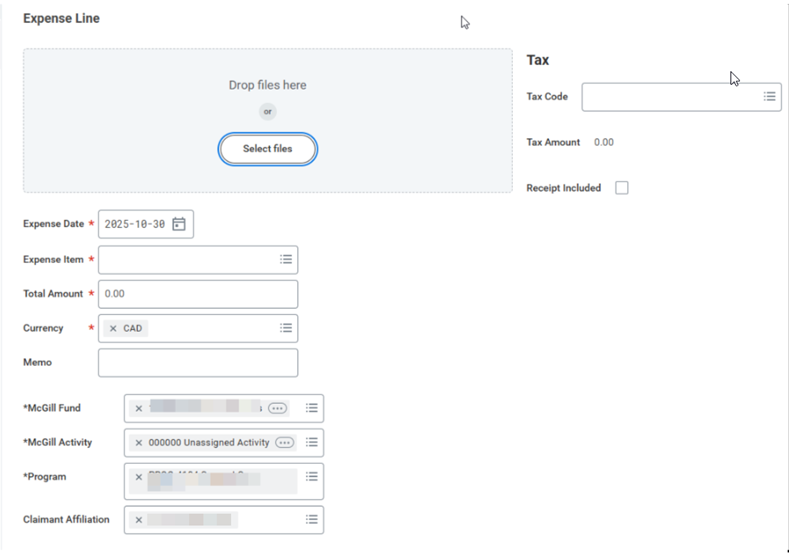
\includegraphics[width=0.65\columnwidth]{Pictures/ExpenseLine.png}
    \end{figure}

    \item Attach the receipt or a copy of the receipt by either dropping the respective file in the attachment section, or by clicking “Select Files” and selecting the appropriate receipt. This is mandatory, and the expense report cannot be submitted without each expense line item having a corresponding attachment. Receipts are not required for the following expense items: meal per diem, lodging allowance, childcare per diem, mileage, tolls, public transportation and gratuities if paid in cash. \\

    \item In the Expense Line section, update/complete the expense item fields as per the information indicated below:

    \begin{figure}[H]
            \centering
            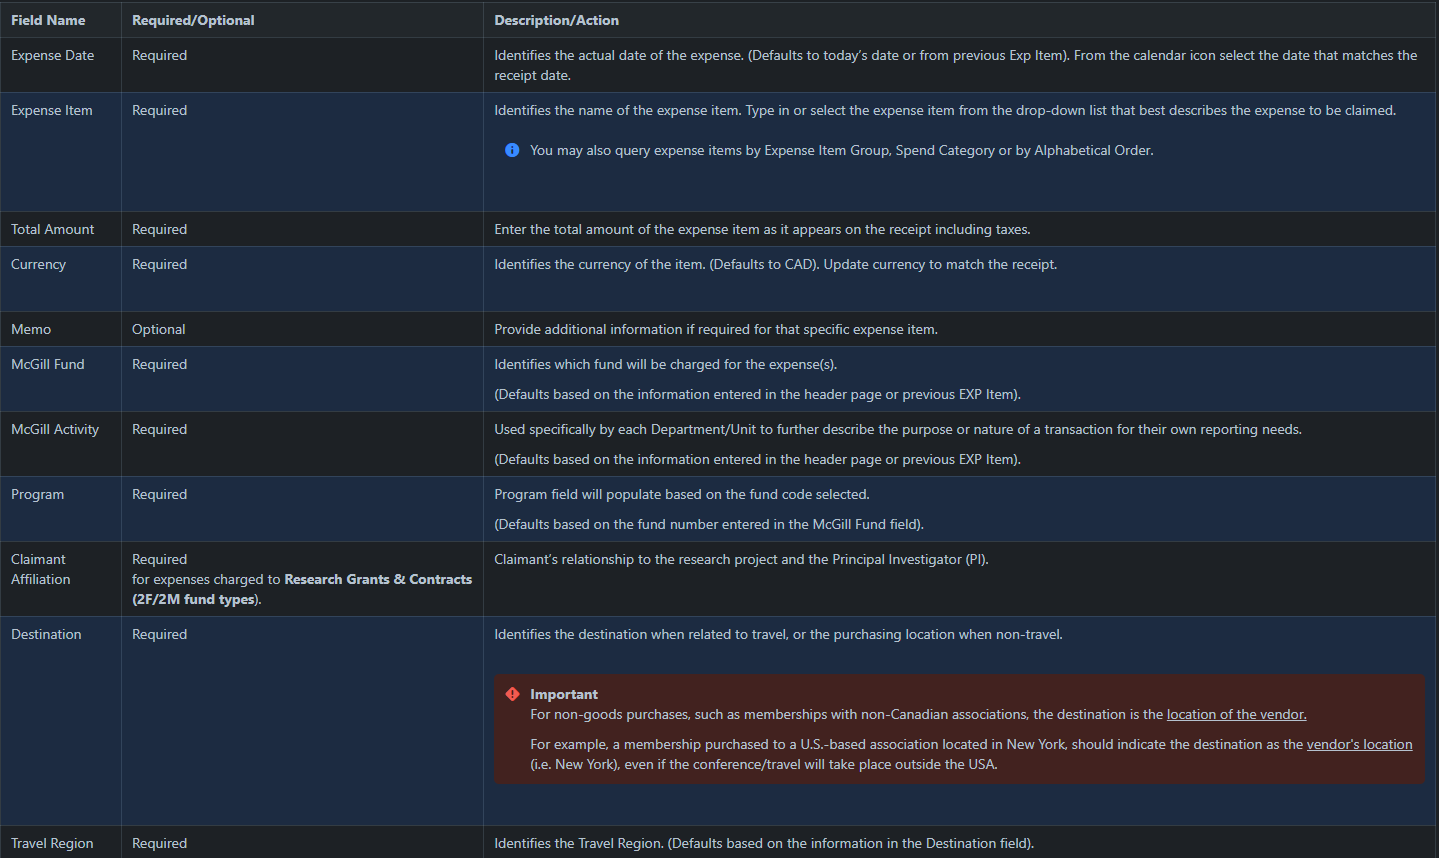
\includegraphics[width=0.8\columnwidth]{Pictures/FormFields2.png}
    \end{figure} 

    \item The tax code and tax amount will populate based on the information entered in the Item Details section. As advised and recommended by McGill University's tax consultants, McGill University has implemented the "factor method" in Workday Expenses. The "factor method" is a tax calculation approach that uses a predetermined factor, therefore tax calculation displayed in WD Expenses may differ from the taxes displayed on receipts. All tax calculations in Workday Expenses (except for airfare, train, chartered bus and seat selection) must NOT be overridden. \\

    \textbf{\color{ocre}Important:} The taxes are only to be overridden to match what is indicated on the receipt for the following expense items: airfare, bus chartered, seat selection fees and train. \\

    \item Should additional expense lines be required, click on “Add”. Repeat steps 12-17 as needed. If alerts and/or error notifications display, click on the notification to expand and read the message. Click on the ‘X’ to exit the alert/error message. 

    \begin{plaincorollary}
 \textbf{\color{ocre}Tip:} The following receipts may be grouped by purchasing location and entered as a single item:
    \begin{itemize}
        \item Parking
        \item Gas
        \item Taxi - if travel related. Local (Montr\'eal) taxi receipts for McGill staff must be entered as individual items with a detailed explanation for each receipt.
        \item Per Diem
        \item Postage
        \item Tolls
        \item Calling cards
    \end{itemize}   
    \end{plaincorollary}
    

    \item Once all expense lines have been entered, select one of the following options below:

    \begin{figure}[H]
            \centering
            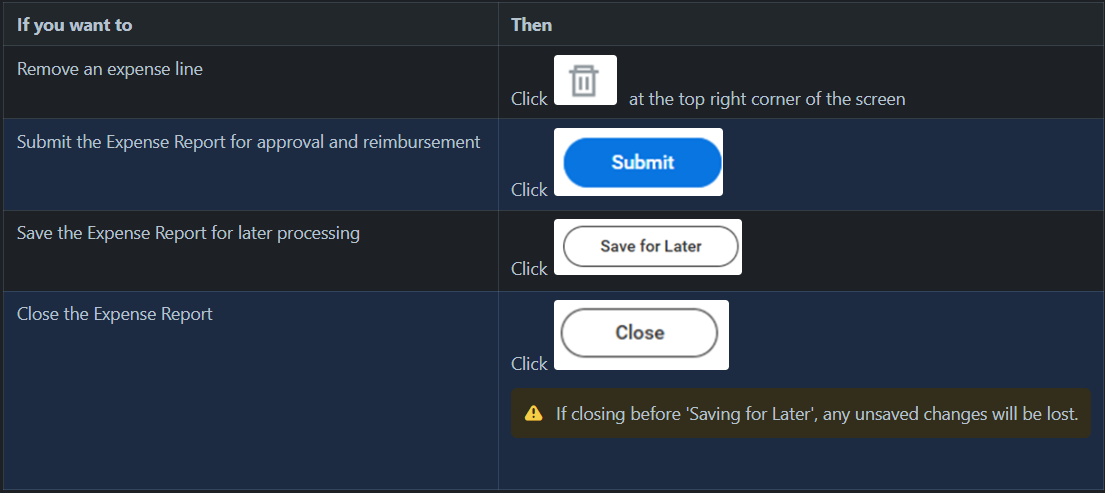
\includegraphics[width=0.8\columnwidth]{Pictures/Step19.png}
    \end{figure}
    \item  Once the expense report is submitted, a message will display to indicate the expense report was successfully submitted, and routed to an Expense Partner’s approval’s queue.

    \begin{figure}[H]
            \centering
            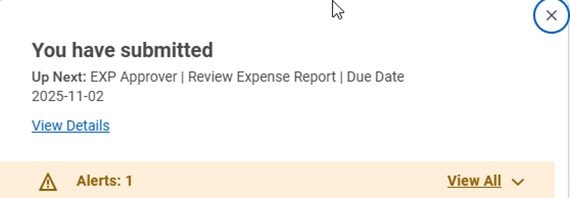
\includegraphics[width=0.8\columnwidth]{Pictures/ReportSubmitted.png}
    \end{figure}

    \item Once the expense report is reviewed and approved by all approvers (Expense Partner(s) and FFM(s)), the expense report is settled for payment.\\
    
\end{enumerate}    

    
    \subsection{Jira Ticket (Summer)} \index{Reimbursement} \index{Jira Ticket}
    \noindent A great step by step tutorial for the Jira ticket process is available at the   \href{https://general-knowledgebase.mcgill.ca/spaces/FSKB/pages/133300374/Student+Grad+Undergrad+-+How+to+Submit+an+Expense+Report}{McGill General Knowledge Base.} The guide is for an expense reimbursement, but the procedure for a cash advance is nearly identical. A guide for the Workday process follows this one. The guide has also been transcribed here for archival reasons.
    
    \noindent As a student, you must complete and submit the Student Expense Reimbursement JIRA form via the Finance Service Desk Portal: \url{https://hrservicedesk.mcgill.ca/servicedesk/customer/portal/12}.
    
    \noindent Before you begin the reimbursement process, make sure you have the \textbf{fund number, activity code, supporting documents} and \textbf{receipts} and the \textbf{name of your supervisor/Principal Investigator}. Also ensure that your banking information is up to date on Minerva. Refer below to additional information on these required data.

     \noindent \textbf{Fund Number:} Six-digit code that should be provided by your supervisor/Principal Investigator prior to incurring “other” expenses, including travel.
     
     \noindent \textbf{Activity Code:} Also provided by your supervisor/Principal Investigator. If none is provided, use the default code: 000000.

    \noindent \textbf{Supporting documents/receipts:} Required for all expenses being claimed except for mileage claims, meal per diems, tolls, public transportation and gratuities if paid in cash. All receipts must include:
    \begin{itemize}
        \item Identification of the supplier
        \item Supplier’s GST and QST number, when applicable
        \item Name of claimant, when applicable (e.g., hotel, airfare, registration)
        \item Full description of expense
        \item Total amount paid, along with proof of payment indication.\\
    \end{itemize}
     
     \noindent \textbf{\color{ocre}Note:} If you have received a travel award, submit only the portion of your expenses that exceeds the amount of the award (for example, if your travel award was \$500 and your total expenses were \$1,000 you should only submit the remaining \$500). If your total expenses are less than the amount of the award, do not submit an expense report. Instead, contact your Graduate Program Coordinator (GPC) to arrange for the unused funds to be returned to the university.\\
     
    
    \begin{plainexercise}
    \textbf{\sffamily \normalsize As per the Travel and Other Expenses Policy:} 
           
    Expense reports related to travel, trips (including field trips) and conferences must be submitted no later than \textbf{30 days} following the return date. 
    
    Expense reports not related to travel, trips (including field trips) or conferences that are submitted after \textbf{90 days} following the oldest receipt date will not be reimbursed.
    \end{plainexercise}


 

    
     \noindent \textbf{\sffamily Step-by-step Instructions}

     \begin{enumerate}[leftmargin=10pt]
         \item Log in the \href{https://hrservicedesk.mcgill.ca/servicedesk/customer/portal/12}{Finance Service Desk Portal.}\\

         \item Under `McGill Student (Grad \& Undergrad) Expense Reimbursements \& Spend Authorizations', select the Expense Reimbursements request form. If you're applying for a cash advnce instead, select the Cash Advance form instead.

            \begin{figure}[H]
                    \centering
                    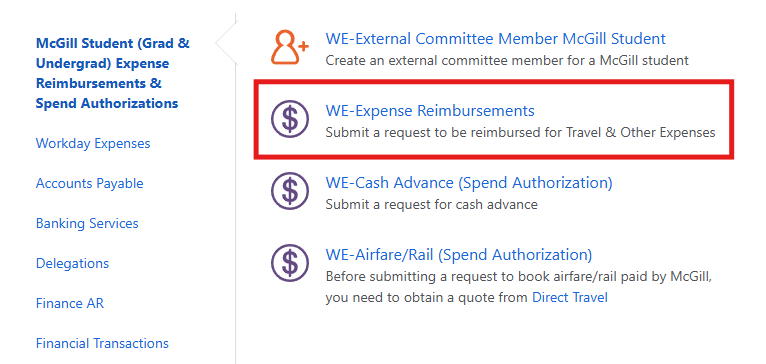
\includegraphics[width=0.8\columnwidth]{Pictures/Expense_Reimbursement.png}
            \end{figure}
            
        \item Select that you are completing this request for yourself.\\

        \item Select your student status, i.e., Graduate or Undergraduate.\\

        \item Select if you received a travel award. Note: If yes, upload the travel award confirmation letter in the Attachment section.\\

        \item Provide a brief description of your reimbursement request, e.g., “NAME OF CONFERENCE -November 2025”.\\

        \item Type in and select the name of your supervisor/Principal Investigator.\\

        \item Enter the 6-digit fund code provided by your supervisor/Principal Investigator. If you need to charge more than one fund, use the Expense Description box to indicate the distribution of expense amounts to each fund, enter the additional fund codes, along with their respective activity codes.\\

        \item Enter the activity code to be charged for all expenses. If it’s unknown, use 000000.\\
    
        \item Select the reason for your request by selecting from the drop-down menu in the Purpose of Expense field.\\
    
        \item Choose the start and end date of your expense/travel by clicking the calendar icon.\\
    
        \item Indicate if this trip/travel included personal dates/travel. Note: If you select yes, provide the dates/expenses which are not related to university-related travel in the respective field.\\
    
        \item Enter your destination (city, province/state). For non-travel related expenses, please enter Montr\'eal, Qu\'ebec.\\
    
       \item Select the destination country from the drop-down menu.\\

       \item In the Expense Description field, provide details of the expense, such as:
    \begin{itemize}
        \item Complete name of the conference, purpose, etc.
        \item Indicate any amounts not to be reimbursed, e.g., personal amounts, travel awards coverage.
        \item If you need to charge more than one fund, indicate the distribution of expense amounts to each fund, enter the additional fund codes, along with their respective activity codes.For more information, refer to section PR7.1.8 of the \href{https://www.mcgill.ca/financialservices/policies/reimburse/procedures}{Procedures for Travel \& Other Expenses.}\\
    \end{itemize}

        \item Attach all receipts or clear photos of receipts pertaining to the expenses for which you are claiming reimbursement.Note: Upload each receipt separately. Do not combine all receipts in 1 PDF.
    
    \begin{itemize}
        \item In the case of airfare with costs that are not necessarily a consequence of travel on behalf of McGill, a quote for the itinerary purely related to the university business must also be attached.\\
    \end{itemize}

        \item Acknowledge that your banking information is up to date on Minerva; all expenses claimed are accurate complete and legitimate; and, that any false or misleading claims may result in an obligation to return the funds to McGill University.\\

        \item Click the Create button. A ticket with its respective number will then be generated. You will also receive that information by email.\\
        
     \end{enumerate}

  
    
    \noindent \textbf{\sffamily What to expect after submitting a claim?}
    
    The claims will be processed by Finance Service Desk and approved by your Faculty/Administrative Unit’s Expense Partner, who will be added to the ticket. This will happen in Workday Expenses, and you will be notified when it happens. If the Expense Partner requires additional information from you, they will use the ticket to communicate with you. Ensure you monitor your inbox and/or the ticket in the link provided to avoid any delays in processing the claim. Once the Expense Partner reviews and approves the claim, the expense report is en route to the supervisor(s)/Principal Investigator(s) responsible for the fund(s) being charged for approval. Once all approvals are recorded, you will receive an email notification that the funds will be deposited into your bank account within 48 hours, and the ticket will be closed in the Finance Service Desk Portal.
    
    

\section{Stipend and Tuition} \index{Stipend} \index{Tuition}
The most up to date information about tuition and financing can be found on the McGill Physics \href{https://www.physics.mcgill.ca/grads/finance.html}{website}.

As of the 2026/2027 academic year, the net annual tuition fee for a McGill Physics graduate student is {\color{ocre}\$5,722.05} (\$3,321.83 + \$2,400.22) and {\color{ocre} \$6,435.31} (\$4,035.09 + \$2,400.22) for International Students after departmental subsidies for non-Québec students.

There are certain fees that are opt-outable when you go on \textit{Minerva > Student Menu > Student Accounts Menu > Student Fee Opt-outs}. Opt out period is limited to the two weeks prior to the fee payment deadline in September and in late January. Check \href{https://www.mcgill.ca/student-accounts/tuition-fees/fee-descriptions}{the fee descriptions} to understand your fees and make an informed decision on whether to pay them or not.

Typically, a Physics student receives financial support in the form of a stipend and teaching assistantship income (see section \hyperref[TA]{\textcolor{purble}{\ref*{TA}}}).

For the 2026/27 academic year, non-scholarship students will receive a stipend of {\color{ocre}\$27,061}, contingent upon satisfactory progress toward the degree, within the normal time frame for its completion. Students holding an external award or scholarship that is less than \$27,061 will receive a stipend such that the total of the scholarship and the stipend is \$27,061.

\subsection*{TA-ship income} \index{Teaching Assistantship}

Graduate students may apply for TAships of approximately \$6,922 totalling 180 TA hours over the course of the academic year. The conditions of TAships are governed by a collective agreement, and graduate students are considered to be in a ‘priority pool’ for the first two years of their MSc program, and the first five years of their PhD program. TAships are not compulsory, and while the department typically is able to offer TAships to all priority pool students, this cannot be guaranteed.
    

\section{Scholarships and Awards} \index{Scholarships}\label{section:scholarships}
Some common sources of funding are listed below.

\subsection{Natural Sciences and Engineering Research Council of Canada (NSERC)} \index{Scholarships! NSERC}
\begin{itemize}
    \item \href{https://nserc-crsng.canada.ca/en/funding/funding-opportunity}{All funding opportunities}
    \item \href{https://nserc-crsng.canada.ca/en/funding-opportunity/canada-graduate-research-scholarship-masters-program}{Canada Graduate Research Scholarship - Master's program} -- December 1st deadline
    \item \href{https://nserc-crsng.canada.ca/en/funding-opportunity/canada-graduate-research-scholarship-doctoral-program}{Canada Graduate Research Scholarship - Doctoral program} -- Check McGill's \href{https://www.mcgill.ca/gps/funding/fac-staff/awards/tri-agency-cgrs-d-cihr-nserc-sshrc}{internal deadline} (typically mid September)
\end{itemize}

\begin{plainexercise}
    If you apply for NSERC CGRS D as a McGill student, you must go through the internal application process first because McGill has a doctoral award quota. The internal deadline is typically a month earlier than the Direct To Agency deadline. You will be notified if your application is selected to be forwarded to the federal level.
\end{plainexercise}

International students enrolled in Canadian institutions are eligible to apply for NSERC CGRS D but only up to 15\% of the available awards can be allotted to them.

If you enter into the doctoral program straight from Bachelor's, consider applying for the NSERC CGRS M for your first year to maximize your funding period.

Consult the eligibility criteria for your desired scholarship carefully. In general, the eligibility windows are:
\begin{itemize}
    \item Master's students -- for CGRS M: 0 to 12 months of full time studies in the MSc program
    \item Direct entry PhD students (from a Bachelor's program):
        \begin{itemize}
            \item For CGRS M: 0 to 12 months of full time studies in the PhD program
            \item For CGRS D: 0 to 36 months of full time studies in the PhD program
            \end{itemize}
    \item PhD students after obtaining a MSc -- for CGRS D: 0 to 36 months of full time studies in the PhD program
    \item PhD students fast-tracked from a MSc program: 0 to 36 months of full times studies in the PhD program (meaning, the counter only starts when you officially become a PhD student).
\end{itemize}

The well-known secret of this system is that you can start applying for NSERC scholarships the year prior to the start of your program. For example, a student entering the MSc program in Fall 2027 can apply for NSERC CGRS M in Fall 2026. However, you can only apply for NSERC CGRS D at most three times. 
    
\subsection{Fonds de recherche du Québec (FRQ)}\index{Scholarships! FRQ}
    \begin{itemize}
        \item \href{https://www.mcgill.ca/gps/funding/intl/provincial-agency-awards}{Master's Research Scholarships}
        \item \href{https://www.mcgill.ca/gps/funding/intl/provincial-agency-awards}{Doctoral Research Scholarships}  
    \end{itemize}
\begin{plainexercise}
    Unlike NSERC, FRQNT applications are submitted directly to the agency at \href{https://frqnet.frq.gouv.qc.ca/}{FRQnet}. However, McGill requires that students complete a FRQ application details \href{https://www.mcgill.ca/gps/funding/intl/provincial-agency-awards}{form}. 
    
    The abstract for your application must be submitted in French. McGill's GPS offer the translation service on a rolling deadline basis, consult \href{https://www.mcgill.ca/gps/funding/intl/provincial-agency-awards/preparing-frq-doctoral-competition}{this page}.
\end{plainexercise}
The eligibility window for FRQNT is quite similar to NSERC (more details are provided above), with a small nuance of FRQ counting full-time study terms instead of months (3 terms instead of 12 months, and 14 terms instead of 36 months). The deadline is usually \textbf{October 1st}.

\subsection{Internal Scholarships} \index{Scholarships! Internal}

You will receive an email with detailed instructions around May each year.

\subsection{Other scholarships} \index{Scholarships! Others}
\begin{itemize}
    \item \href{https://www.mcgill.ca/gps/funding/opportunities/masters}{Master's students} 
    \item \href{https://www.mcgill.ca/gps/funding/opportunities/phd}{PhD students} 
    \item \href{https://www.mcgill.ca/studentaid/scholarships-aid/graduate}{All graduate students}
\end{itemize}

\begin{plainexercise}
    McGill holds fellowship information sessions for major awards, usually around August every year. It is a good opportunity to come ask questions and get tips on crafting a good application. Check this \href{https://www.mcgill.ca/gps/funding/maximize-my-chances/workshops-information-sessions-and-webinars}{page}.
    
    Also keep an eye out in your McGill email inbox for information about application workshops and reviews.
\end{plainexercise}

Beyond the scholarships listed above, it is also possible in some cases to apply to privately funded scholarships, such as the \href{https://www.janestreet.com/join-jane-street/programs-and-events/graduate-research-fellowship/}{Jane Street Graduate Research Fellowship}. These scholarships will frequently be advertised in your emails, though it may be the case that some you might have to personally search for depending on your specific research and situation.

\subsection{Top-ups} \index{Top-ups}
All students holding a scholarship/award of a value less than \$40,000 per year receive an award top-up bonus, in addition to the stipend described above. Holders of NSERC and FRQNT scholarships with a value of less than \$30,000 per year receive an award top-up bonus of \$6,500. Holders of other scholarships and awards will receive an award top-up bonus equivalent to 20\% of the value of their awards, up to a maximum total amount of award plus top-up of \$40,000. Top-up bonus for holders of scholarships and fellowships of a value greater than \$40,000 is left at the discretion of the supervisor.

If the scholarship or fellowship includes an amount to cover the extra tuition fees paid by international students, that amount will first be subtracted before calculating the top-up.

    
    \section{Personal finances} \index{Personal Finances}
Personal finance is extremely important to set yourself up for success in the future. The reality is that most grad students don't make much money so having clear financial planning can also be a matter of survival.

We recommend going through \href{https://mcgillpersonalfinance.com/}{this free online} course offered by McGill for the foundation of budgeting, saving, and investing. In this section, we take a deep dive into the world of finance to give you at least the confidence to take the next steps of optimizing your finances. We try to address all the commonly asked questions about finances from years of mentoring new students settling in Canada/Montr\'eal.

\textbf{\color{ocre}Disclaimer:} The author is just a physics graduate student who happens to be very interested in personal finance and, therefore, volunteered to write this guide. They don't have formal financial advising accreditation so take their words as mere suggestions and do your due diligence in verifying the following information. 

\subsection{Banking} \index{Banking}
Banking in Canada is very well regulated. Therefore, there is really no wrong choice in picking a bank in Canada (as long as it's a reputable institution, your money will be safe). 

There are 3 categories of options:

\subsubsection{Traditional brick and mortar banks
}

The Canadian banking sector is dominated by the Big Five banks: Royal Bank of Canada (RBC), Toronto-Dominion Bank (TD), Bank of Nova Scotia (Scotiabank), Bank of Montr\'eal (BMO), and Canadian Imperial Bank of Commerce (CIBC).

There is very little to differentiate between them in terms of experience, fees, and perks. They all have branches close to McGill. You can choose based on vibes and it won't make much of a difference. Often, they will run a promotion for opening an account with them (i.e. get a free ipad/ipod/mac) so choose one with the best offer at the moment.

The nice thing about them is that you have physical branches all over country to walk into and talk with a real person. However, they are slow to innovate and tend to have higher fees and fewer rewards as compared to their online competitors.

\subsubsection{Credit unions
}

A credit union is a member-owned nonprofit cooperative financial institution, and they tend to offer very similar services to a bank. They have more of a local feel to them, and the services tend to be more personable. The biggest one in Québec is Desjardins. 

\subsubsection{Online-only banks}

This is where it gets interesting. They offer no fee banking and higher saving interest rates than a traditional bank. The limitation is that you don't have a physical branch (but how often do you need to go to a bank anyway?) and online support (phone, email, chat) can be frustrating.

Some options that work in Québec:
\begin{itemize}
    \item \href{https://www.wealthsimple.com/en-ca}{Wealthsimple}: It is a fintech platform that is quite popular, especially to young Canadians, for its simple no-fee investing tools and high baseline interest chequing accounts. Their accounts are free to open, they reimburse ATM fees for cash withdrawal, their cash card has no foreign exchange (FX) fees. They also offer a good credit card but (or plus, depending how you feel) they gamify saving and investing through frequent giveaway contests. They also run a great pay-what-you-can online tax filing service.
    \item \href{https://www.eqbank.ca/ }{EQ Bank}: They consistently offer the best interest rates for your savings/chequing account. They also reimburse ATM fees. Their cash card has no FX fees while giving 0.5\% cashback on transactions.  
    \item \href{https://www.tangerine.ca/en/personal}{Tangerine}: They are a subsidiary of Scotiabank, but they operate independently. They offer full daily banking suites (meaning you get a true debit card, unlike the above two) and attractive (but for a limited time) promo rates for their saving accounts.
    \item \href{https://www.pcfinancial.ca/en/pc-money-account/}{PC Money Account}: This is linked to one of the biggest grocery reward programs in Canada. They have high saving interest rates, no FX fees, no monthly fees, and spending cashback in the forms of reward points. 
\end{itemize}

\begin{plaincorollary}
    These digital banks often run promotions for account opening as well. Reach out to fellow graduate students for referrals for extra perks.
\end{plaincorollary}


\subsection{Credit Cards} \index{Credit Cards}
In Canada, a credit score is used to determine your likelihood of repaying a loan. You need it to get a mortgage, finance a car purchase, or in some cases to rent a place so it is important to start building your credit history in Canada early especially if you are planning to work and live in Canada in the long term. The easiest way to do so is by obtaining a credit card and using it responsibly.  

You can read up on credit score and report in Canada \href{https://www.canada.ca/en/financial-consumer-agency/services/credit-reports-score/credit-report-score-basics.html}{here}. Note that you can view your credit reports for free from Canada's main credit bureaus, Equifax and TransUnion. Furthermore, as a Québec resident, you have the right to lock and unlock your credit reports to prevent identity theft.

All that said, if you don't have good financial habits (ie. you tend to spend more than you have), credit cards can be dangerous to your financial future. 

Alright, let's dive right into the world of credit cards!

\subsubsection{Must know about credit card use}
If you've never gotten a credit card before, it is very important to understand how it works to maximize rewards and avoid fees. Here, we will outline the few must know basics, but you can get more details \href{https://www.canada.ca/en/financial-consumer-agency/services/credit-cards/credit-card-work.html}{here}. 

Your billing period is typically a month (28 -- 31 days). All the transactions you made in that month will count toward your owing balance on your statement at the end of the period. You will then have at least 21 days of interest free grace period (per federal regulations) to make your payment. \textsc{\color{ocre}You must make your payment in full to avoid any interest charges.} Credit cards typically charge very high interest rates (19\% to 29\% annually, compounding daily!) so a missed or partial payment means that you must pay exorbitant interests on every purchase you made for that whole period until it is paid off.

Scary! How do you avoid this? We recommend \textsc{\color{ocre} setting up automatic payment for your credit card}! If you wish to pay manually, you still can -- the autopay only kicks in at the end of the grace period if you have not paid your balance in full, so it helps you avoid any interest fees. In fact, it makes mathematical sense not paying manually and letting autopay do its job because the money you leave in your chequing account can keep accumulating saving interests (the good kind!) during the grace period. However, it is a good idea to look at your statement once a month to check for any unauthorized transactions and understand how much you've spent!

The caveat is of course to make sure you have enough money in the account to which you link the autopay to avoid any non-sufficient funds (NSF) fee.

You'll have a certain credit limit, ie. the maximum amount you can borrow at any given time. If you have no credit history, your limit will be very low. So, you might need to pay it off more often to continue using it throughout the month. Or you might have to ask for one-time limit increase to make big purchases (for example, to pay conference registration fees). 

{\color{ocre}Important}: Avoid cash advances or cash-like transactions (essentially getting cash from your credit card!) because the interest rate is astronomically high and there is no grace period for them. Don't spend what you don't have to begin with but if desperate, look into student loans or low interest lines of credit from your bank first. 

\subsubsection{Your first credit card}
If you are new to Canada, you can get a Newcomer or Student credit card from any traditional bank you open an account with. Sometimes, the bank might require an in-person appointment to approve your first card. A secured card (you put money in the card before you can use, so functionally more like a debit card) can also be a good starter, especially if you don't know if you can use a credit card responsibly.

These “beginner” cards don't have super exciting perks so there is not much differentiation between cards. The purpose of your first card is simply to build your credit history here then you can get better cards down the line (if you want).

If you have a banking history but not necessary credit history in Canada (as in you have an account with the same bank since forever but never had a credit card before), you might be able to talk to your bank to get a more decent credit card. In such case, you can try for the cards in the next section first.

If you have/had an American credit card (especially AMEX), it's worth checking with your Canadian bank if they can open for you a good card by pulling your American credit history. 

Some decent student credit cards (as of Aug 2026) to consider:
\begin{itemize}
    \item BMO CashBack Mastercard for Student -- no annual fee, 3\% cashback on groceries, 0.5\% for other purchases
    \item Desjardins Cash Back Mastercard/Visa -- no annual fee, 2\% cashback on dining, entertainment, alternative transportation and pre-authorized payment, 0.5\% otherwise
    \item RBC Cash Back Mastercard -- no annual fee, 2\% cashback on groceries, 1\% otherwise after the first \$7000 spent per year.
    \item Scotiabank Scene+ Visa Card (for students) -- no annual fees, 2 Scene points per \$1 spent for certain grocery stores, home hardware stores, and Cineplex, 1 Scene point per \$1 otherwise (1 Scene point is valued at 1 cent per point)
    \item CIBC Dividend Visa Card for Students -- no annual fees, 2\% cashback on groceries, 1\% on certain categories
\end{itemize}

\subsubsection{Good general credit cards}

If you're in the category of "just make it simple" user, cashback cards are the easiest because you don't have to think about maximizing your point redemption. The author recommends having a Visa and a Mastercard, which will cover the majority of use cases and serve as a backup for each other. AMEX has some very nice cards as well but in Québec, its acceptance rate remains quite low, so check that the places you frequently shop at would accept it before getting one.

In general, knowing how much you spend per month (by tracking your spending a few months after moving to Québec) helps you select the best card for yourself. For example, if your biggest expense is usually groceries, you can choose a card with high cashback on groceries. 

You could of course get multiple cards that reward different categories if you are keen on maximizing your returns. There is a tradeoff between simplicity and profits so it's up to you what you want.

Also, don't be afraid to get a credit card with an annual fee if the maths works out (but don't go crazy paying for multiple high fee cards). 

Another thing to look for when choosing a credit card is insurance such as extended warranty and travel insurance. If you often rent a car for weekend trips, car rental insurance could save you hundreds in not having to purchase insurance add-ons.

One caveat is that cards with fees usually require a minimum income so you might have to first establish a banking relationship with an institution then talk them into giving you the card you want. One possible maneuver is “upgrading” your existing no fee card.

There are simply way too many credit cards to highlight in this little guide section. So we recommend reading these 2 Globe \& Mail articles:
\begin{itemize}
    \item Guide for people interested in \href{https://www.theglobeandmail.com/business/article-cash-back-credit-cards-guide-canada/?utm_medium=RedditAd%20and%20utm_campaign=traffic_mkt}{cash-back cards}.
    \item Guide for people interested in \href{https://www.theglobeandmail.com/business/article-travel-credit-cards-guide-canada/?utm_medium=RedditAd%20and%20utm_campaign=traffic_mkt}{travel cards} (ie. good for travel perks)
\end{itemize}

You can also use \href{https://www.finlywealth.com/credit-cards/compare}{this tool} to filter out credit card that best suits your usage.

That said, here are a few underrated credit cards:
\begin{itemize}
    \item \textbf{Rogers Mastercard:} No annual fee, 1.5\% on everything (if not a Rogers customer) or 2\% on everything and 5\% on Rogers services as a Rogers customer. The World Elite version has comprehensive insurance (but notably no travel insurance).
    \item \textbf{Wealthsimple Visa:} No foreign exchange fee, 2\% on everything, comprehensive insurance (but notably no car rental insurance). Annual fee is waived under certain conditions. 
    \item \textbf{Canadian Tire Triangle Mastercard:} No annual fee, 3\% on groceries, 1\% otherwise as CT money to use in their stores. You can pay a lot of bills through their portal to earn 1\% back on bills you normally can't pay with a credit card (tuition for example!). Similarly, the World Elite version has comprehensive insurance and free roadside assistance (especially good if you plan to drive during Canadian winter!) 

\end{itemize}

    The first two are great options if you just want to use one card for everything. 

\subsubsection{Play the credit card game}

    No, we're not talking about credit card churning (it's a whole different beast!). We're talking about getting money / points back for every cent you spend, especially for bills that take up a big percentage of your monthly expenses that you normally can't pay with a credit card like rent, tuition, and utilities.

    The easiest way is to use PC Money account to pay your monthly bills. You get up to \$5 per month in PC Optimum points to pay bills through them. It works like any normal bank account so there is no extra hassle and it's easy to open an account. 

    A similar way, already mentioned at the end of the previous section, is using the Canadian Tire Triangle Mastercard because they have a peculiar feature of letting you pay bills as if you're paying from a normal bank account. This gets you 1\% back from your bills but the downside is that you can only spend the cashback at certain stores.  

    Another way is to use \href{https://chexy.co/}{Chexy} paired with the Scotia Momentum Visa Infinite + Card. Chexy lets you pay any bill with the credit card, and codes the payments as recurring. Recurring payments give you 4\% back, but you pay 1.75\% fee to Chexy, so it nets you a bit more than 2.25\% for these payments. You can use it for utilities and tuition -- you only need to set it up once and automate it for monthly bills. There are other similar services.


\subsection{Investing} \index{Investing}

In recent years, Canada has seen a surge in amazing investing platforms with low to no fee stock and ETF trading. The two platforms that paved the way for regular Canadians are \href{https://www.questrade.com/}{Questrade} and \href{https://www.wealthsimple.com/en-ca}{Wealthsimple}. They are great and popular options thanks to their intuitive UI and \$0 commission stock and ETF trading.

That said, most major banks offer commission-free trading for a selected list of ETFs (exchange-traded funds). If you are a buy-and-hold type of investor (which you should be!), you should be able to find an ETF that fits your needs with most brokerages.

These platforms are in competition with each other, so they offer frequent promotions. Be sure to catch one for your account opening!

Furthermore, it'd be wise to understand and utilize different types of tax advantaged saving accounts offered by the federal government to grow your money as efficiently as possible. See section \hyperref[accounts]{\textcolor{purble}{\ref*{accounts}}} -- in general, most graduate students benefit from maxing out their TFSA first.

If you are new to investing or unfamiliar with the Canadian market, understandably it seems very daunting. There is a lot of information out there. Here are some Canada-specific resources:
\begin{itemize}
    \item McGill free personal finance \href{https://mcgillpersonalfinance.com/}{online course}
    \item Book: \textit{The Wealthy Barber 2025: The Fully Updated All-Time Canadian Classic} -- Dave Chilton
    \item Ben Felix \href{https://www.youtube.com/@BenFelixCSI/playlists}{YouTube channel}
    \item The Canadian Couch Potato \href{https://canadiancouchpotato.com/}{website}
    \item The Canadian Portfolio Manager \href{https://canadianportfoliomanagerblog.com/model-etf-portfolios/}{blog}
\end{itemize}

The common time-tested advice is to not try and pick individual stock or time the market. Consistent investment in a broad market index fund regardless of market conditions will most likely beat individual stock picking and mutual funds with high fees thanks to the power of compounding.

In Canada, there are three popular suits of ETFs that are very similar to each other that cover different asset allocations (bonds to stocks ratio) to suit your needs. They are from Vanguard (XEQT, XGRO, XBAL), BlackRock (VEQT, VGRO, VBAL), and BMO (ZEQT, ZGRO, ZBAL). Depending on your risk tolerance and current financial health, they can be a good option for index investing. \href{https://canadianportfoliomanagerblog.com/model-etf-portfolios/}{This guide} outlines what is in each ETF and goes through the process of choosing what's appropriate for you.


An example scenario of someone who takes reasonable steps to begin index investing looks like this:

\begin{plaincorollary}

Bob started graduate school in September. He receives \$2,000 monthly as his stipends. 

By November, his life has settled down in Montréal. He was able to track and determine that his monthly expenses are at most \$1,500. He also wants to set aside \$100 as a "fun" fund. He would like to save and invest \$400.

Since he does not have any debt or savings, he starts by building an emergency fund that would cover his essential expenses for 3 months. He sets aside \$400 as soon as he receives his stipends every month into a high interest savings account (HISA) that yields 2.75\% annually with his bank. He also puts all the leftover at the end of the month to this emergency fund.

After building his emergency fund, Bob opens a TFSA in a direct investing platform knowing that he has unused contribution room. He intends to leave his investment alone for 30 years. After assessing his financial health and risk tolerance, Bob decides to invest in an ETF that tracks the global stock market with a bias toward Canada. He carefully selects the version that has 0 commission fee on his investing platform of choice.

Now, with every paycheque, instead of leaving it in the HISA, he immediately uses \$400 to buy the selected ETF. Even if the market goes down, he does not panic sell and keeps his course. When there are unforeseen circumstances, he draws on his emergency fund then rebuilds it before continuing his investment.
\end{plaincorollary}

Of course, the above example is not a one-size-fits-all. A good action plan also varies depending on if you have any debt (prioritize paying down your high interest debts first), or if you have other immediate financial goals (in which case, save for your goals separately in a safe vehicle like HISA or GIC), or if you are earning high taxable income (in which case, RRSP might be a better account type to start with).


\subsection{Miscellaneous (phone \& internet, learning French, discounts, etc.)}

\subsubsection{Phone and internet} \index{Phone} \index{Internet}

Canada is covered by Big Three telecom providers: Bell (BCE), Rogers Communications, and Telus. In Québec, we have a strong regional provider in Qu\'ebecor (Videotron) as well.

Phone and internet plans directly under these big companies can be quite pricey. However, they have discount subsidiaries that are significantly cheaper while operating on the same network. The caveat is that the subsidiaries are focused on digital-first (or -only) self service so it is aimed toward more tech-savvy people.

Some mobile provider brands to check out: Fizz, Public Mobile, Fido, Freedom Mobile, Koodo, Chatr, Lucky, and PC Mobile.

In terms of internet, Bell and Videotron are the biggest players in Québec. However, Fizz, EBOX, and oxio (a rare independent provider!) are good alternatives.

To get the best possible rates, check specifically for student deals and deals around Black Friday, Boxing Day, and major holidays. Another tactic, albeit time consuming, is to pitch companies against each other by threatening to leave for their competitor. For example, you get in an online chat with both Bell and Videotron at the same time and have them argue what they can offer to have you as a client!

\subsubsection{Learning French} \index{French}
A detailed guide is available in section \hyperref[section:french]{\textcolor{purble}{\ref*{section:french}}}. If you are interested in learning French, there are two great free options:
\begin{itemize}
    \item \href{https://www.quebec.ca/en/education/learn-french}{\textit{Francisation} by the Government of Qu\'ebec}: It is completely free (although the waitlist can be long). They also give a stipend to full-time participants.
    \item \href{https://www.mcgill.ca/skillsets/files/skillsets/gps_award_for_french_classes.pdf}{GPS French Course Award}: The Graduate and Postdoctoral Studies (GPS) office covers the registration and copyright fees of ONE eligible French course at the French Language Center for selected recipients. Registration and application are available the term preceding the course.  
\end{itemize}

\subsubsection{Free and discounted things} \label{discounts} \index{Discounts}

McGill Student Services already compiled a \href{https://www.mcgill.ca/studentaid/files/studentaid/cheap_sheet_2025_final_updated_1125.pdf}{massive list}, this section will highlight a few options that are more likely to be relevant to a physics grad student living near the downtown campus.

If you struggle to make ends meet, McGill and the greater Montr\'eal community have a few food bank and free grocery programs: \index{Food banks}
        \begin{itemize}
            \item \href{https://snacmcgill.wixsite.com/snac}{Student Nutrition Accessibility Club }
            \item \href{https://yellowdoor.org/connections-over-food/}{The Yellow Door}
            \item \href{https://www.moissonmontreal.org/en/}{Moisson Montréal}
        \end{itemize}

Cheap and/or discounted groceries: \index{Groceries}
\begin{itemize}
    \item \href{https://www.bulkbarn.ca/home-en/index_deals.html}{Bulk Barn}: Bulk snacks and ingredients. They have a 15\% student discount on Wednesdays
and offer 15\% off your order on Sundays when you bring a re-useable container.
\item \href{https://www.maxi.ca/fr}{Maxi}: offers price match, so it saves you time from
hunting down deals in multiple stores. Show them the sale item at the other store at checkout and
they will match the price.
\item \href{https://groupeadonis.ca/en}{Marché Adonis }: A discount market (10\% off with a student ID). Check their weekly flyer for their best deals. Consider coming here especially if
you're looking for specialty Greek ingredients.
\item \href{https://www.marchenewon.com/en}{Marché Newon}: offers a very wide variety of Asian products as well as fruits and vegetables at reasonable prices.
\item Segal's Market (4001 Blvd St-Laurent): small, cheap grocery store with a good, quality
selection. Segal's is great for cheap produce, dairy, and organic products. Good for stocking up in bulk for less. Get hemp milk for the best price. However, their meat/poultry selection is limited.
\item \href{https://www.facebook.com/mcgillfarmersmarket/}{McGill's Farmers’ Market} (available from July to October)   
\item \href{https://www.superc.ca/en/student-discount}{Super C}: Offers 10\% off from Monday to Wednesday purchases of \$50 or more upon presentation of a valid student card.
    \item \href{https://www.metro.ca/en/products-to-discover/grocery/whats-new/metro-avenue-parc}{Metro Parc Ave}: It is not a cheap grocery store (in fact, their prices are on the higher end) but if this is your only or most convenient option, they have 10\% off purchases of \$50 or more upon presentation of a valid student card from Monday to Wednesday.
    \item \href{https://www.provigo.ca/en}{Provigo}: Similar to Metro, it is another expensive store but it offers 10\% back in reward points on Mondays for students.

\end{itemize}

You can definitely enjoy life in Montréal on a budget. Here are cool things that are free or are at reduced price for students and young adults (more details can be found in section \hyperref[exploreMTL]{\textcolor{purble}{\ref*{exploreMTL}}}):
        \begin{itemize}
        \item \href{https://www.mbam.qc.ca/en/information/discounts-and-free-offers/}{Montr\'eal Museum of Fine Arts}
            \item \href{https://www.mcgill.ca/travelservices/transport/book-vehicle}{Cheap car rental} 
            \item \href{https://www.osm.ca/en/single-tickets/}{Orchestre symphonique de Montréal }
            \item \href{https://operademontreal.com/en/young-adult-opera-tickets}{Opéra de Montréal} 
            \item \href{https://orchestremetropolitain.com/en/education-at-the-om/}{Orchestre Métropolitain}
            \item \href{https://espacestdenis.com/fr/rabais-etudiants/}{Espace St-Denis} 
            \item Buy \href{https://montreal.ca/en/articles/acces-montreal-card-exclusive-offers-and-discounts-5990}{Accès Montréal card} for \$11 to get discounts on many activities and establishments in Montréal for one year.
        \end{itemize}

\section{Taxes} \index{Taxes} \label{tax}
It is your responsibility to file taxes in Canada. As graduate students on low income, you are very likely to receive benefit and credit payments from the federal and provincial governments, so filing taxes is also in your best interest.

You will need to file taxes federally and provincially:
\begin{itemize}
    \item \href{https://www.canada.ca/en/services/taxes/income-tax/personal-income-tax.html}{Canadian Revenue Agency} 
    \item \href{https://www.revenuquebec.ca/en/citizens/income-tax-return/}{Revenu Québec}
\end{itemize}    

The easiest way to do so is by using a certified tax software, the approved list can be found \href{https://www.canada.ca/en/services/taxes/income-tax/personal-income-tax/how-file/tax-software/find-software.html}{here}. If you file as a Québec resident, the list of approved software from Revenue Québec is smaller, and can be found \href{https://www.revenuquebec.ca/en/partners/authorized-products/authorized-software/personal-income-tax-return-individuals/}{here}. It is recommended to use a service approved by both agencies to reduce the tax workload for yourself. 

If you are a Canadian from another province, you can choose to file in your home province, as you are considered a visitor to Québec for the purpose of full-time studies. Choosing to file in your home province saves you time on transferring your driver's license and your health card to Québec (for which the process can be arduous).  

\begin{plainexercise}
    \href{https://www.canada.ca/en/revenue-agency/services/tax/individuals/topics/important-dates-individuals.html}{Key dates} to be aware of:
\begin{itemize}
    \item Earliest day to file your taxes online: middle of February
    \item Deadline to file your taxes: April 30
    \item Deadline to file your taxes if you or your spouse or common-law partner were self-employed in 2025: middle of June
\end{itemize}\vspace{-15pt}
\end{plainexercise}

You can follow \href{https://www.canada.ca/en/services/taxes/income-tax/personal-income-tax/how-file/tax-software/complete-return.html}{the linked steps} to file your personal income taxes electronically. This section will highlight specifically how to gather tax slips from McGill on \href{https://horizon.mcgill.ca/pban1/twbkwbis.P_WWWLogin}{Minerva}:
\begin{itemize}
    \item \textbf{Tuition Tax Receipts}: T2202 and Relevé 8 are found in Student Menu >  Student Accounts Menu > Student Tax Menu > Tuition Tax Receipts Menu 
    \item \textbf{Scholarship, Bursary and Fellowship Awards Tax Receipts}: T4A and Relevé 1 are found in Student Menu >  Student Accounts Menu > Student Tax Menu > Tax Slips (Scholarship, Bursary and Fellowship Awards) 
    \item  \textbf{Student Housing Tax Slip}: Relevé 31 are found in Student Menu >  Student Accounts Menu > Student Tax Menu > Student Housing Tax Slip
    \item \textbf{TA tax slips}: Your T4 and Relevé 1 can be found electronically in \href{https://wd3.myworkday.com/mcgill/d/home.htmld}{Workday} (only accessible during your active TA period) in Menu > Pay, Benefits \& Compensation > Pay > All Tax Documents. Otherwise, they are also mailed to you during the tax season.
\end{itemize}

You can take advantage of the different types of savings accounts, to minimize taxes on your hard earned money in the long run: 

\subsubsection{Tax-free savings account (TFSA)} 
\index{TFSA} \label{accounts}

TFSA is a registered savings account that can hold both cash savings and investments. Any saving interests or investment income (including capital gains and dividends) generated inside a TFSA are completely tax free. 

\href{https://www.canada.ca/en/revenue-agency/services/tax/individuals/topics/tax-free-savings-account.html}{This government page} outlines all you need to know. A simplified summary to know follows:
\begin{itemize}
    \item A Canadian resident of at least 18 years of age can contribute to their TFSA at any time as long as they have the available contribution room (calculate \href{https://www.canada.ca/en/revenue-agency/services/tax/individuals/topics/tax-free-savings-account/contributing/calculate-room.html}{here}).
    \item You can withdraw from TFSA tax-free whenever you want. You regain the contribution room equal to the withdrawn amount plus the new annual TFSA dollar limit the next calendar year.
\end{itemize}

There is an important distinction that your contribution room is not the same as your account value. Consider:
\begin{itemize}
    \item Alice puts in \$7,000 to max out her TFSA contribution room. Her account grows to \$10,000. She can withdraw \$10,000 tax free and regain \$10,000 in contribution room plus the new limit the following calendar year.
    \item Charlie puts in \$7,000 to max out his TFSA contribution room. He lost all of it in risky investment in penny stocks. He cannot simply contribute \$7,000 to compensate, he effectively lost his contribution room. He needs to wait until the following calendar year to get the new limit.
\end{itemize}

That is to say, it is advisable to start your TFSA early to reap maximum benefits of the account, but one needs to be prudent with the type of investment to make.

\subsubsection{Registered Retirement Savings Plan (RRSP)} \index{RRSP}
As the name suggests, an RRSP is meant for Canadians to save for retirement. Contributions to the RRSP can be used to reduce your tax. Your money can (usually) grow tax free inside the RRSP but you generally pay taxes upon withdrawal from the RRSP. Read up on it \href{https://www.canada.ca/en/revenue-agency/services/tax/individuals/topics/rrsps-related-plans/registered-retirement-savings-plan-rrsp.html}{here}.

The common use case for the RRSP is to defer taxes from high income years (where your tax bracket is high) to low income years, usually retirement (when you are required to pay less taxes). 

For the majority of graduate students, their earnings are well below the basic personal amount, meaning they are likely not required to pay taxes. In fact, it is likely their high income years are in the future, and therefore an RRSP is more beneficial later down the line.

\subsubsection{First Home Savings Account (FHSA)} \index{FHSA}
FHSA is a registered account that lets first-time home buyers to save to buy their first home tax-free. All information can be found \href{https://www.canada.ca/en/revenue-agency/services/tax/individuals/topics/first-home-savings-account.html}{here}. 

FHSA combines the best of TFSA and RRSP but with a time limit. Any contribution you make to your FHSA can be use to reduce taxes, money can grow inside tax-free, and withdrawal can also be made tax-free for qualified purposes (ie. to buy your first home). Qualified withdrawal must be made within 15 years of first opening an account. Otherwise, your FHSA can be converted into RRSP without affecting your RRSP contribution room, effectively giving you "extra" RRSP contribution.

A key different is that your FHSA contribution has an annual contribution limit of \$8,000 and a lifetime maximum contribution limit of \$40,000. You can carry forward up to \$8,000 of unused contribution room from a previous year once the account is open, making the absolute maximum contribution in any single year \$16,000.

You might consider opening a FHSA if you are planning to buy your first home in the next 15 years.        
\chapterimage{TA.pdf}
\chapterimagecaption{\textit{The Night Before The Exam
} (1895) by Leonid Pasternak}

\chapter{TAing}

    
\section{What is a TA?}

A Teaching Assistant (TA) is a graduate student who assists an instructor in conducting a course. Their duties include but are not limited to teaching concepts, organizing tutorials and office hours, aiding with labs, grading assignments and exams, and invigilation. All TAs are members of the \href{https://tsum-stsem.ca/}{ Teaching Support Union at McGill (TSUM)}, formerly known as the Association of Graduate Students Employed at McGill (AGSEM). \\

%\begin{plainbox}
%\noindent \textbf{\sffamily Who can become a TA?} \\
%All \textbf{graduate students} at McGill are eligible to apply for a TAship. 
%\end{plainbox}

\noindent \textbf{\sffamily How do I become a TA?} \index{Teaching Assistantship!Application}\\
All graduate students have the right to apply for a TAship and they will be hired after submitting an application form to a department
(Hiring Unit). You can apply for and work TA positions in departments other than your own. There is only one application process per term for each Hiring Unit. You'll receive an email from the Graduate Program Coordinator (GPD) when the application is live. TA positions are  posted on Workday by: \vspace{5pt}
\begin{itemize}
    \item For Fall courses: 3rd Monday of May,
    \item For Winter courses: 3rd Monday of October,
    \item For Summer courses: 2nd Monday of March.
\end{itemize}

\begin{plaincorollary}
Students need to apply as an external candidate on Workday for the Fall postings since they won't have access to their work email. All postings will be up for at least 14 calendar days and you will be notified withing 35 days of the application deadline. 
\end{plaincorollary}


\noindent \textbf{\sffamily What does a TA contract look like?} \index{Teaching Assistantship!Contract}
\begin{plainexercise}
  All TAs work for 90 hours per semester. The maximum size of a TA position is 180 hours per academic year. The rate of pay for 2026-27 is \textbf{\$38.46 per hour} so a student is eligible for \$6922.8 before taxes for the combined year 2026-27 (Fall + Winter).   
\end{plainexercise}
Our \href{https://tsum-stsem.ca/documents/Simplified%20CA%20August%202024.pdf}{Collective Agreement (CA)} is set to expire on July 31, 2027 after which a new contract will take its place. A CA is a written legal contract between an employer (McGill) and the union that outlines the rules and conditions for the workers (TAs). 

TA salaries are paid \textbf{biweekly}, and the pay schedule is available on your Workday dashboard and on \href{https://www.mcgill.ca/hr/files/hr/2026_salaried_pay_calendar.pdf}{McGill's website.} Each payday is for approximately 12 hours (except for the first one) so you can expect a recurring payment of roughly \$420 every 2 weeks. \\

\noindent \textbf{\sffamily What happens after I accept my offer?} \\
You must accept a TA offer via the Workday portal within \textbf{7 days} of receiving an
offer letter. There are exceptions to the 7 day rule due to documented
illness. If you are offered a position that is later withdrawn, you must be offered a vacant position of at least the same size. After accepting your offer, at the beginning of the semester, you must: 

\begin{enumerate}
    \item \textbf{Complete the onboarding on Workday.} This involves verifying your personal information and checking your tax contributions such as RRSP or TFSA. \\

    \item \textbf{Fill the \href{https://tsum-stsem.ca/members/membership-forms/}{Union Membership Form}} for full union membership. All TAs are considered members of the union, regardless of whether they fill the membership form. However, if the visible strength of the union falls below a certain number, the union may cease to exist so it is highly recommended.\\

    \item \textbf{Meet with the instructor} to discuss your tasks and divide them between you and other TAs. The instructor should also provide you access to the myCourses page of the course and possibly Crowdmark if they plan on using it for grading. \\

    \item \textbf{Fill out the \href{https://www.mcgill.ca/hr/files/hr/agsem_ta_workload_form_en-fillable.pdf}{Workload Form.}} It is a very useful tool that provides a structured approach to
    formally negotiate your workload, maintain a detailed record of your hours, and request additional hours if needed. 

    \begin{plainbox}
        Students must ensure that they don't work more than the \textbf{90 hours} per semester limit. If the course instructor forces you to go over this limit, contact your \href{https://tsum-stsem.ca/contact/}{ \underline{department delegate}} immediately. 
    \end{plainbox}

    \item \textbf{Access your work email}. Students should now be able to access their work email that ends in @mcgill.ca. This email can be used for all communications between students or the course instructor. If you are new student and have not had a @mcgill.ca before, you'd need to set it up via Outlook like you did for your personal email. \\

    \item \textbf{Review your workload form} at the halfway mark of the term and meet with the instructor to review your performance and hour allocation. The midterm review is highly recommended as it helps to adjust the distribution of hours if enrollment has fluctuated or if you feel you need more time for certain tasks. \\
\end{enumerate}



\noindent \textbf{\sffamily Do I have any job security as a TA?} \index{Teaching Assistantship!Priority Pool}\\
TAs are entitled to preferential hiring based on seniority. This is called the
\textbf{Priority Pool} (PP). Every semester, a department must assign any available TA positions to applicants with priority, starting with the highest level of priority. Priority declines as following:

\begin{plaindefinition}
    \begin{itemize}
        \item Fourth-year PhD
        \item Third-year PhD
        \item Second-year PhD
        \item First-year PhD
        \item Second-year Master's
        \item First-year Master's
        \item Fifth-year PhD
    \end{itemize}
\end{plaindefinition}

\noindent You enter the PP once you accept a job in a department and the length of time you have in the PP is determined by the date of your initial enrolment. For example, a PhD4 applicant who has never been a TA in that department before \textbf{does not} have priority. Applicants who are more advanced in their programs may still have priority if they receive extensions to their PP entitlement, for things like field work or maternity leave.

\noindent\textbf{\color{ocre} Note:} Applicants with PP status are given priority for a TA position, but not for
the specific TA position that they want. 

\subsection{What is TSUM?} \index{TSUM}
All TAs are represented by a labour union, the Teaching Support Union at McGill (TSUM). The union changed its name very recently, in April 2026, from Association of Graduate Students Emplyeed at McGill (AGSEM) to TSUM. Hence we'll refer to it as TSUM throughout this document. \\

\noindent \textbf{\sffamily What is a Union?} \\
As a labour union, TSUM represents TAs (Unit 1) and Invigilators (Unit 2) at McGill. Recently, the union also began representing  course-based academic casuals (Unit 3) such as graders, course tutors, undergraduate student course assistants, etc. Hence, the necessary name change. TSUM bargains with the McGill administration to produce Collective Agreements, which are legal documents that protect student workers.

\begin{figure}[htbp]
    \centering
    \begin{subfigure}[b]{0.48\textwidth}
        \centering
        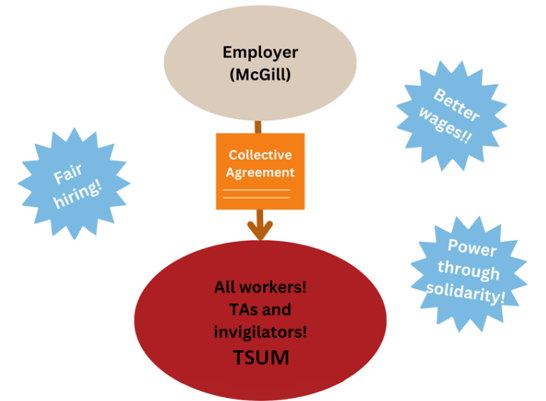
\includegraphics[width=1\linewidth]{Pictures/tsum1.png}
        \caption{How TSUM works.}
        \label{fig:img1}
    \end{subfigure}
    \hfill
    \begin{subfigure}[b]{0.48\textwidth}
        \centering
        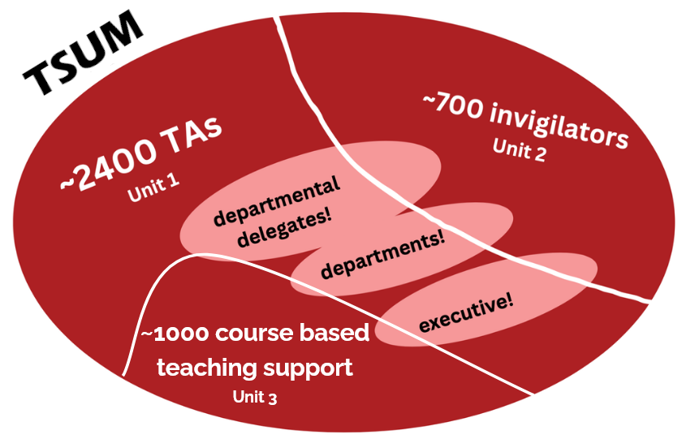
\includegraphics[width=\linewidth]{Pictures/tsum2.png}
        \caption{Members of TSUM.}
        \label{fig:img2}
    \end{subfigure}
    \label{fig:both_images}
\end{figure}

 \noindent The union\textbf{ negotiates on your behalf }and enforces collective agreements with McGill to establish standardized wages, working hours, benefits, and priority rights. The union also defends workers against unfair labor practices, tracks cumulative hours and overtime, and helps members address workplace disputes.

\noindent \textbf{\sffamily What is a Delegate?} \index{TSUM!Delegate}\\
Delegates are your union representatives at the departmental level. Delegates are also your \href{https://mgaps.physics.mcgill.ca/people}{\textbf{first points of contact}} in your union! Delegates engage with TAs in their department via emails, phone calls, and office visits. They also check the tentative hiring list every term to ensure the worker hiring rights are respected and also assist you in filing grievances. In addition, they serve on the Delegate’s Council to assist in union governance. 

\noindent The Physics department currently has 3 delegates. You can contact them via email: \url{https://tsum-stsem.ca/contact/}. \\


\noindent \textbf{\sffamily What else do we do?} \\
We fight for better working conditions through prioritizing regular, meaningful engagement with all of our members. We do this by: 
\begin{itemize}
    \item \textbf{General Assemblies:} TSUM hosts general assemblies \textbf{once per term} and unit assemblies once per year where we discuss workplace issues and solutions and vote on things like bargaining and negotiations, union finances, and leadership. You also get a free meal paid for by the Confédération des Syndicats Nationaux (CSN), our parent labour union! \\
    \item \textbf{Bargaining}: We are currently in the process of pre-bargaining with McGill to renew our CA that is set to expire on July 31, 2027. Regular updates, will soon be available on this \href{https://tsum-stsem.ca/news/}{link.}  \\
    \item \textbf{Grievances:} TSUM solves any disputes that may arise between the university and an employee such as late pays, going over contract hours, unsafe working conditions, etc. To file a grievance, reach out to a delegate or a \href{https://tsum-stsem.ca/your-rights/grievance-frequently-asked-questions/}{TA grievance officer}. \\
    
    \end{itemize}

\noindent \textbf{\sffamily What can you do?}\\
To help our cause you can do the following things: \\
    \begin{enumerate}
    \item \textbf{Sign the \href{https://tsum-stsem.ca/members/membership-forms/}{membership form}.} All TAs are considered members of the union whether or not they sign the card or not, however, if less than 50\% sign the card, the union would require a vote to be certified. Hence, it is highly recommended to sign you card as soon as you become a TA to ensure that the union maintains its strength.  \\ 
    
    \item \textbf{Attend Assemblies}, social gatherings such as rallies, potlucks, BBQs etc. Since TSUM is a democracy, assemblies are where we make major decisions that affect all members of the union. Make your vote count! \\
    
    \item \textbf{Get involved:} TSUM has several open positions in various commitees and working groups. You can also become a \textbf{delegate} or run for an executive position. To become a Physics delegate, you need to nominate yourself at the MGAPS Fall Assembly. \href{https://docs.google.com/forms/d/e/1FAIpQLSd1uaNmDgvsz2AEtq9MbR7N8De4p6-33g2jSGqGDNHRUkmbfA/viewform}{Here's} a general interest form that you can sign if you wish to be involved in mobilization, communications or other TSUM activities.\\
    
    \item \textbf{Bargaining:} Since this year is bargaining year, you can also get involved with the bargaining commitees. Did you know that you can also attend \textbf{open bargaining} sessions between the union and McGill and witness the negotiations in real-time? Stay glued to your email for more information.\\
\end{enumerate}

  \begin{plainexercise}
        \textbf{TA training:} All \textbf{\underline{first time TAs}} get up to 3 hours of paid teaching training, in addition to your contract hours! The training is organized by the Teaching and Learning Services (TLS). To know more, follow this \href{https://www.mcgill.ca/teaching-academic-programs/instructors/programming/ta-training}{link}.
    \end{plainexercise} 


\subsection{Extra hours for TA}   
    In the event that you work over your allotted 90 hours per semester you may request more paid hours from your course supervisor. Your contract guarantees that you get paid for 90 hours of work, so you will at a minimum always get paid for 90 hours of work. 

    Keep track of your hours each week in order to know if you are being over worked. If you do go over hours and don't want to work anymore you don't have to! For any unfinished work the university must offer you the hours required at the TA rate before they are offered to anyone else. But you are under no obligation to accept this offer.

    If your additional hours are no approved you stop working. You cannot be asked or expected to complete free work for the university. If your course supervisor tries to force you to work for free or if your TA work is outsourced to a non TA contact your delegates or TA officer immediately as this is a violation of your rights as a worker.

\section{How to be a Good TA?}
\subsection{Grading}
Grading is one of the most essential TA tasks. Most of your working hours will be spent grading assignment and exams. It is a very good idea to communicate with the instructor early to establish guidelines. Some instructors are very lenient with grading while others have strict guidelines. Regardless, the most important thing is to be \textbf{consistent.} \vspace{5pt}

\begin{itemize}[leftmargin=10pt]
    \item \textbf{Design a good grading rubric.} Spend enough time to make it useful and stick to it. Once you are done grading, give the rubric to the students so that they can verify their solutions.
\end{itemize}
\begin{plaincorollary}
    Quite often, you will need to retroactively change your rubric based on the first few evaluations. That's perfectly fine! Make sure that you go back and grade everyone fairly.
\end{plaincorollary}
\begin{itemize}[leftmargin=10pt]
    \item \textbf{Provide useful feedback.}  Mention explicitly where marks have been lost and the point total per question. All feedback should define the actions a student can take to improve themselves. Make a list of common errors and communicate them to the class in tutorials.\\
    \item In case of \textbf{late submission}, you may contact the student via email and ask for justification. Typically, it's okay to accept late submissions, especially in case of illness or travel or if the student has had prior permission from the instructor. However, the final decision rests at the discretion of the course instructor.\vspace{5pt}
\end{itemize}
\begin{plainexercise}
If you stumble upon \textbf{plagiarized} content, work that's clearly unoriginal, contact the instructor immediately. This is well above your pay-grade as TAs are not expected to deal with such serious offences. 
\end{plainexercise}

\subsection{Tutoring/Office Hours}
Tutorials and office hours are useful for students to get in-depth feedback and ask questions. They also enables you to develop better communication skills.

\begin{itemize}[leftmargin=10pt]
\item \textbf{Spend time} reviewing the concepts and questions a day before. Try solving the problems atleast once without looking at the solutions. \\

\item When solving a problem in class, write each step carefully and legibly and ask students for \textbf{constant feedback} on whether they are able to follow the procedure or whether a particular formula has been taught in class. \\

\item You can always \textbf{divide the class into groups} to work on problems if you wish. You can also ask students to analyze a certain calculation when they go back home if you don't have time to go through it in class. \\

\item During office hours, if students don't have any particular questions, you can go over \textbf{previous quizzes or exam problems}. \\
\end{itemize}

\begin{plaincorollary}
    Students may often ask you questions that you are not prepared for. Don't Panic! You are not the one being tested on your knowledge. Just tell them that you'll get back to them via email or during next class.
\end{plaincorollary} 


\subsection{Labs}
Labs are important opportunities for students to apply their knowledge and gain experimental
skills. It's your responsibility as a lab TA to ensure that students stay on the right track while also letting them learn experimental practices though trial and error. 
\begin{itemize}[leftmargin=10pt]

    \item Ask the instructor for \textbf{clear instructions} and rely on the rubric rather than your own intuition.\\

    \item \textbf{Read} through the entire lab manual or protocol ahead of time and test out calculations or tricky steps.\\
    
    \item \textbf{Communicate objectives} not only with your course supervisor, but also your fellow TAs who will be facilitating the lab with you. \\

    \item \textbf{Use your own experience} as a student to recognize common pitfalls and sources of errors. \\
    
    \item Do not just giveaway the answers to students' questions. However, if you see them struggling, don't wait, 
    \textbf{be proactive} and offer them the necessary help.\\
    \item Make sure that students are aware of universal \textbf{lab safety rules} and ensure that students are not fooling around with equipment, especially instruments that involve electricity.    
\end{itemize}

\begin{plainexercise}
    Always remember to create an \textbf{inclusive} space where students feel comfortable asking questions and sharing their problems. Let them know that there are no silly questions!
\end{plainexercise}

\section{What is the TA Wiki?}\index{TA Wiki}
The \href{https://wiki.hep.physics.mcgill.ca/TAWiki/index.php?title=Main_Page}{TA Wiki} is a brand new initiative undertaken by MGAPS. The purpose of the wiki is to improve continuity between semesters, overcome institutional memory loss, and provide a common space for organizing \textbf{TA-related information and expected responsibilities}. It can be used for the following purposes:
\begin{itemize}
    \item \textbf{TA Hour Logging:} tracking the number of hours worked throughout a semester to maintain transparency for workload. \\
    \item \textbf{Task Breakdown and Expectations:} including descriptions of expected TA duties and recurring responsibilities. \\
    \item \textbf{Information for Future TAs:} for applying to specific TA positions and course-specific tips and recommendations. 
\end{itemize}

\begin{SCfigure}[2][hbt]
    \centering
    
\includegraphics[width=0.3\linewidth]{Pictures/Wikisignup.png}
    \caption*{Since the initiative is in its infancy, we need your help to complete the TA wiki! Just sign up for it and record your experience at the end of the semester. \\

    \textbf{\color{ocre} Note:} You need to make an account to access and edit information on the site. Account creation is currently only possible with admin privileges. Reach out to one of the TSUM delegates or the RTech officer to make an account or simply fill this \href{https://docs.google.com/forms/d/e/1FAIpQLSfjcshi98m5lyCXsSaB7t7WEa-NcOw9MPB3S9mSrw_FOCMVWQ/viewform}{form}. \\
    
    To learn more about the initiative, follow these \href{https://wiki.hep.physics.mcgill.ca/TAWiki/images/f/fd/TAWikiGuide.pdf}{slides.} }
    \label{fig:TAwikisignup}
\end{SCfigure}

\section{Are there non-TA positions?}
If teaching is not your cup of tea, then there are other jobs in the department that you can apply to instead. The pay is equivalent to that of a TAship with a one-year or one-semester long commitment. \\

\noindent \textbf{\sffamily EDI Committee}\index{Coordinators!EDI}\\
The EDI graduate coordinator serves on the EDI committee. The EDI committee strives to make our department workplace more equitable and inclusive. They facilitate ongoing efforts (such as our CEGEP workshops, the Contemporary Physicists website, and others) as well as provide administrative support (such as meeting organization). Additionally, the coordinator also helps the committee organize events such as once-to-twice-a-semester social events and an EDI colloquium. Typically \textbf{1-2 positions} are available each year. \\

\noindent \textbf{\sffamily Outreach Committee}\index{Coordinators!Outreach}\\
The Outreach Coordinators are members of the \href{https://physics-tsi-outreach.physics.mcgill.ca}{Physics \& Trottier Space Institute (TSI) Outreach Committee}. The coordinators work alongside and receive support from the committee, which meets regularly to plan, schedule, and organize our outreach events. There are currently 4 student coordinator positions across the two departments: Hackathon (Physics), Public Talks \& SciComm (Physics), Space Explorers (TSI) and Science in Space (TSI). \\

\begin{itemize}[leftmargin=10pt]
    \item \textbf{Hackathon Coordinator} \index{Coordinators!Hackathon} is responsible for organizing and delivering the annual Physics Hackathon, with support from the Outreach Committee. The coordinator's main responsibilities include: planning and coordinating the weekend-long event, securing sponsorships, and training and recruiting volunteers, mentors, and judges.
\begin{figure}[hbt]
    \centering
    
\includegraphics[width=0.7\linewidth]{Pictures/Hackathon.png}
    \label{fig:hack}
\end{figure} \\
 \item \textbf{Public Talks \& Science Communication Coordinator} \index{Coordinators!Public Talks} organizes public talks and creates content for social media and the outreach website. The coordinator's main tasks are recruiting speakers for the monthly talks, finding venues, advertising talks, coordinating volunteers, and creating and posting content to Physics social media accounts.\\

\item \textbf{Space Explorers Coordinator} \index{Coordinators!Space Explorers} is responsible for running the Space Explorers program, which brings fun, inquiry-based activities to elementary schools throughout Montr\'eal. They must recruit, communicate with, and train volunteers to deliver the program in schools and coordinate with schools to schedule visits. \\

\item \textbf{Science in Space Coordinator} \index{Coordinators!Science in Space} organizes and manages the Science in Space program in which middle school students of under-represented genders in physics build telescopes in Minecraft over a period of \~10 weeks. They are expected to deliver hands-on lectures and coordinate with schools to schedule visits. 
\end{itemize}

\noindent In addition, there are other jobs outside of the department you can apply through Workday as a replacement for TAship. 

\section{More FAQs?}
\begin{itemize}[leftmargin=10pt]
    \item \textbf{Where can I read more about good TA practices?} \newline
    You can refer to the previous  \href{https://mgaps.physics.mcgill.ca/files/Physics-TA-Handbook.pdf}{MGAPS TA Handbook} compiled by Benjamin Dringoli for more knowledge. Despite being a more than few years old, you'd find the content to be very useful.\\
    \item \textbf{Where can I turn for support as a TA and a graduate student?} \vspace{5pt}
    \begin{itemize}
        \item Teaching and Learning Services McGill:\url{www.mcgill.ca/tls}
        \item The Labour Union (TSUM): \url{https://tsum-stsem.ca/}
        \item SKILLSETS McGill: \url{http://www.mcgill.ca/skillsets/offerings/ta-trainings}\\
    \end{itemize}
    
    \item \textbf{Who do I reach out to in case of disputes?} 
    The TSUM delegates are the \href{https://mgaps.physics.mcgill.ca/people}{\textbf{first points of contact}} if you have any questions. Depending on your specific case, they'll forward your complaint to the respective authority. See \href{https://tsum-stsem.ca/your-rights/grievance-frequently-asked-questions/}{this} page for more details. \\
   
    \item \textbf{How much tax do I pay?}\index{Taxes!TA Salary}\\
    The TA stipend is taxable and the amount of tax depends on the duration you have TAed for. Some of the amount is non-refundable but you could get back $\sim \$100-\$200$ when you file taxes at the end of the year. Here's a short overview of what taxes you pay on your stipend as of 2026:
    \begin{itemize}
        \item \textbf{Union Dues:} 2.5\% (non-refundable)
        \item \textbf{Employment Insurance (EI):} 1.3\% (non-refundable)
        \item \textbf{Provincial Parental Insurance Plan (PPIP):} 0.43\% (non-refundable)
        \item \textbf{Quebec Pension Plan (QPP):} exempt up to \$3500, thereon 6.3\% (refund depending on your gross income).
    \end{itemize}
    
    %\item \textbf{Auto deposit?}

\end{itemize}
\label{TA}
\chapterimage{supervisor.pdf}
\chapterimagecaption{\textit{The Lesson}  (1892) by George Goodwin Kilburne}

\chapter{Supervisor Relations}

    Your relationship with your supervisor is a very significant part of your graduate degree, as they will be the first point of contact for many of your concerns. Supervisors receive training before they take on students and should be prepared to address your questions and concerns effectively, however some of them may have done the training a long time ago and may be a little behind the times. \href{https://www.mcgill.ca/gradsupervision/supervisors/mcgill-expectations-graduate-supervision}{This page} on the McGill website provides a basic outline of what the expectations are for supervisors. 

    \section{Letter of Understanding and Progress Reports}\index{Letter of Understanding}\index{Progress Reports}
        
        To ensure accountability on both sides, McGill requires that you fill out "Progress Tracking" forms. Doctoral students are required to fill out a progress tracking form every year as a part of their degree requirements. Master's students are not explicitly required to fill out a progress tracking form as a part of their degree requirements, but they are heavily encouraged to do so.
        \\\\
        \href{https://www.mcgill.ca/gps/files/gps/gps_graduate_student_research_progress_tracking_report_2025_fillable.pdf}{This} is a link to the standard GPS progress tracking form. Broadly speaking the purpose of this is to write down a list of reasonable goals at the beginning of the year to provide accountability both for your supervisor and for you. You are evaluated on whether or not you have achieved the written goals at the next progress tracking meeting (next year), and the evaluation also involves a lengthy justification section (if your progress is unsatisfactory). This section requires your supervisory committee to reference specific aspects of your previous objectives section, and this should inform how you pick objectives when sitting down with your supervisor at the beginning of the year. GPS has \href{https://www.mcgill.ca/gradsupervision/supervisees/discussing-expectations}{this} webpage that is a little bit more detailed about the intention behind writing a letter of understanding.
        \\\\
        The department also provides a guidelines document (which appears to be a Faculty of Science document from 2022) \href{https://www.physics.mcgill.ca/grads/lou22.pdf}{here}. This document is much more specific about what exactly should be discussed at a progress tracking meeting, and has a list of suggestions for additional topics.

    \section{Switching Supervisors}
        It is possible that you may need to switch supervisors during your degree. This can happen for a number of reasons, and in the event that either you or your supervisor feel that you need to end the supervisory relationship your department chair will assist you in finding a new supervisor. GPS has \href{https://www.mcgill.ca/gps/files/gps/graduate_student_supervision_change_of_supervisor_guidelines_april_2026.pdf}{this} document, this is written for department chairs but it describes what the process would be like for you as well. GPS also has \href{https://www.youtube.com/watch?v=4IuLZEAB_aU&t=6s}{this} video going over some things to consider and how to go about the process. The video is also described at the bottom of \href{https://www.mcgill.ca/gradsupervision/supervisees/conflict-resolution}{this} webpage.

    \section{How to file complaints}\label{section:supercomp}
        If you are having difficulty with your supervisor, your first point of contact is the graduate program director (Nikolas Provatas). If this is not an avenue you feel comfortable taking or if you have already tried this without success, there are a number of other options that you can take. GPS provides \href{https://www.mcgill.ca/gradsupervision/supervisees/conflict-resolution}{this} webpage describing the avenues you have to pursue a complaint, along with the summarizing graphic below. The gist is that ideally you want to address the complaint locally first (i.e. with your supervisor, with the graduate program director, chair, or other professors in your department), then move up to more official avenues through the GPS and the university. There are a series of additional offices in the university that are able to help with conflict resolution which are listed on the right of the figure below.

        \begin{figure}[H]
            \centering
            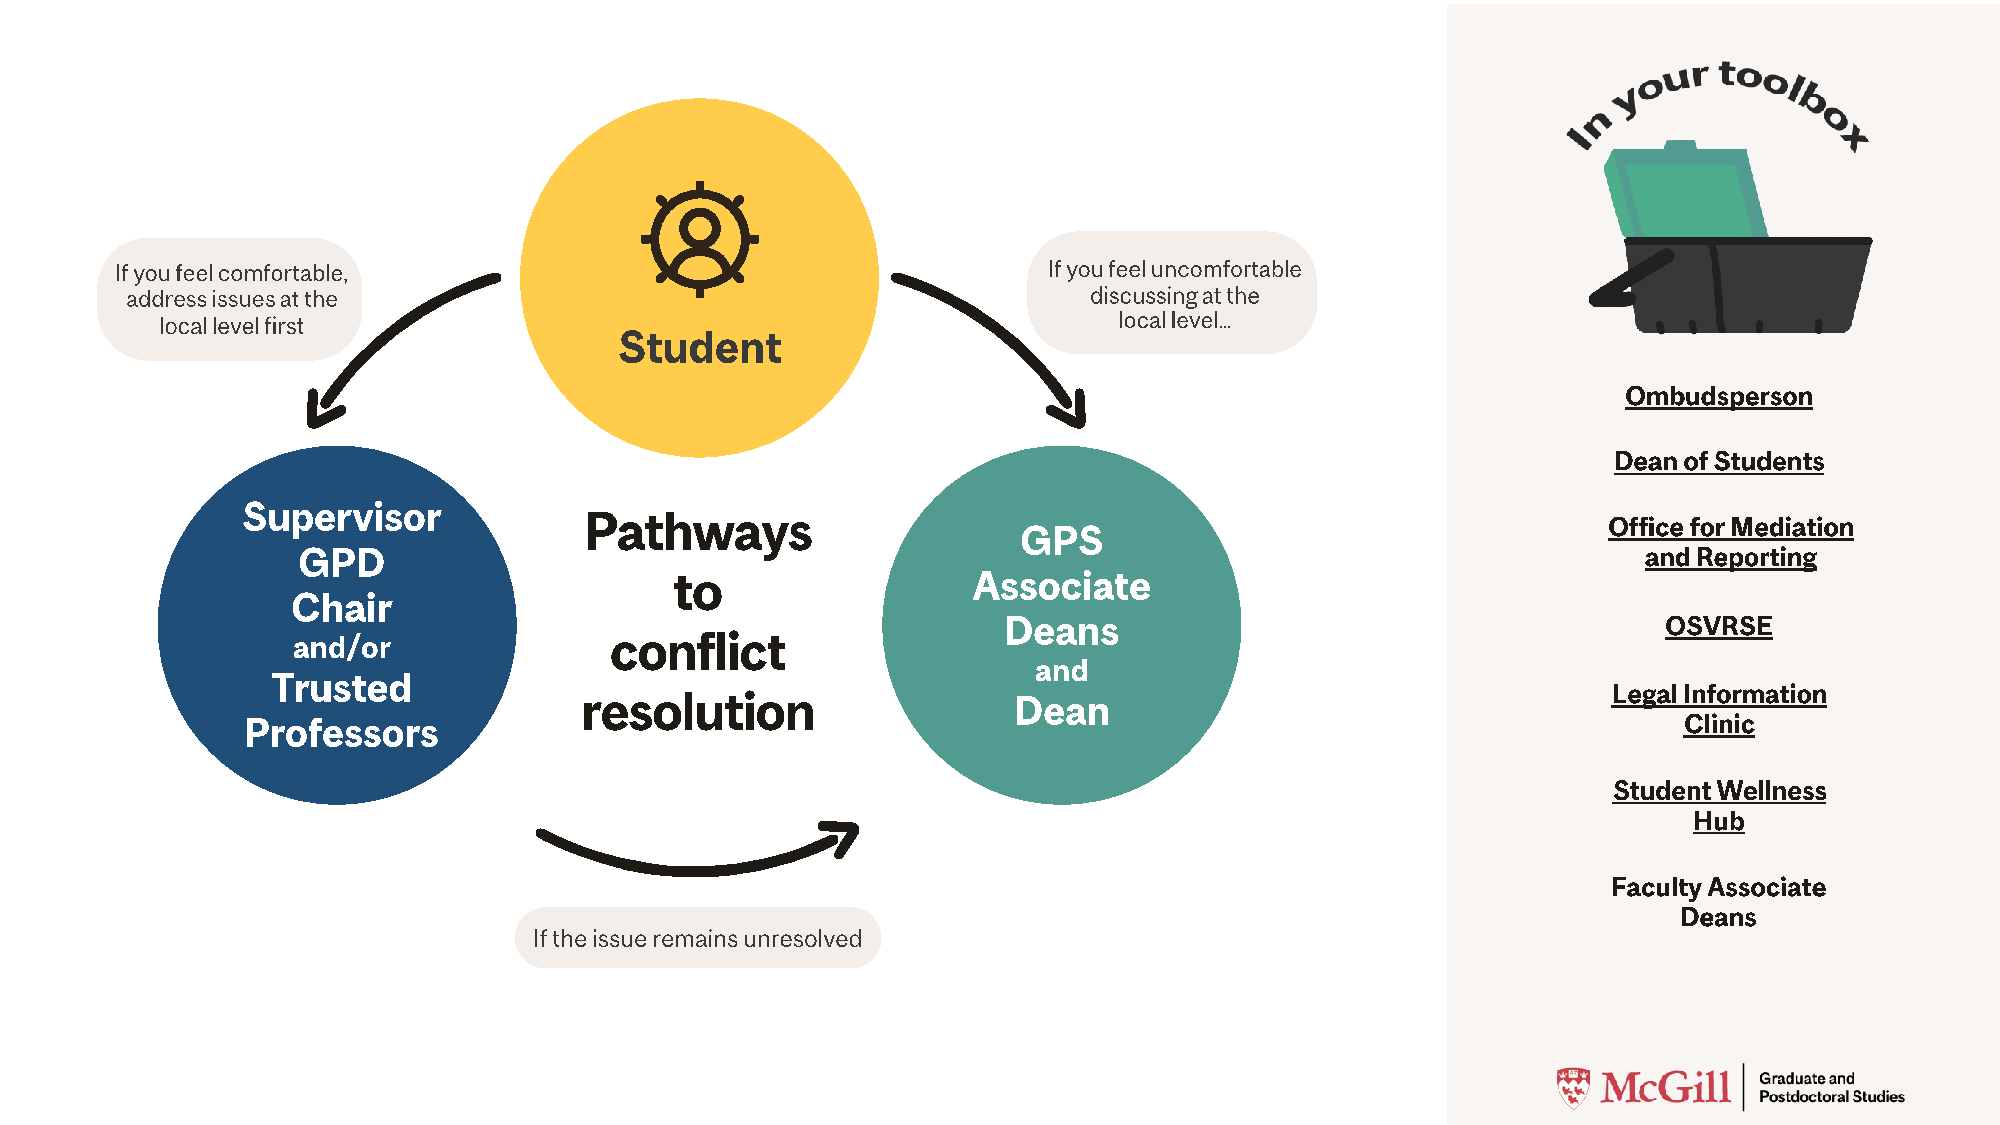
\includegraphics[width=0.95\columnwidth]{Pictures/conflict_resolution_flowchart.pdf}
        \end{figure}
        
        GPS also provides supervisors with \href{https://www.mcgill.ca/gradsupervision/supervisors/resolving-conflict}{this} webpage on resolving conflict, which can inform how you go about addressing a conflict with your supervisor before reaching out to the program director.
\chapterimage{special.pdf}
\chapterimagecaption{\textit{Ophelia}  (1852) by John Everett Millais}

\chapter{Special Situations}

Here is a compilation of some special extraordinary circumstances that could hinder your degree progression.

\section{Academics \& Research}

\subsection{Prelim timing for direct-entry PhD students}   \index{Prelim}     
        In this subsection, ``direct-entry PhD" refers to students who join the PhD program with no previous experience in a graduate physics program---i.e. as PhD 1. Students who enter the PhD program as PhD 2, whether via the McGill fast track, with an MSc from McGill, or an MSc from a prior institution, are not considered direct-entry. 
        
        The general advice is to take the PhD preliminary exam by the end of one's first term of PhD 3 study--e.g. for a student who entered in the fall as PhD2 via fast-track, this would be the fall of the following year; or for a student who entered in the winter as PhD2 with an MSc from another institution, this would be the winter of the following year. Fortunately, this logic extends to direct-entry students---for example, a direct-entry student who joins McGill graduate physics studies in Fall 2026 must take their prelim by the end of Fall 2028.

        However, this is not well-documented on the department website's table of hypothetical prelim timing situations---possibly because direct-entry admissions are not widespread across all parts of the department. At the time of writing, several direct-entry students who embarked upon their McGill graduate physics studies in Fall 2024 and Fall 2025 successfully confirmed with the Physics GPC that they should plan on taking their prelims by the end of Fall 2026 and Fall 2027, respectively; confirming the ``end of first term of PhD 3" rule. 
        
        Please note, however, that, as of Summer 2026, MyProgress is not configured to represent this edge case well: it shows the prelim milestone as overdue for direct-entry students at the end of their fourth non-summer term (as opposed to fifth non-summer term, the GPC-confirmed policy).

    \subsection{Failing a course}\index{Failing a course}

    
    Failing a course can be scary but we promise its not the end of the world. Your options after your first failure (i.e, any grade less than a B-- or any incomplete grade such as J,K, or L) are as follows:
        \begin{itemize}
            \item Contest the grading with the professor (not much can actually be done but always worth an attempt)
            \item Write a supplemental exam upon approval by the department and professor
            \item Retake the failed course
            \item Substitute the failed course by completing an equivalent course. Neither this nor retaking the original class will replace the original failed grade on your transcript.
        \end{itemize}
        Students who fail a second course will be automatically be withdrawn from the University. 

    \subsection{Withdrawing} \index{Withdrawing}
        Harking back to the earlier section, a student will be withdrawn from the University if they:
        \begin{itemize}
            \item Fail two courses
            \item Obtain two unsatisfactory progress tracking reports and the academic unit recommends they be withdrawn
            \item Fail one course and receive one unsatisfactory progress tracking report and is recommended to be withdrawn by their academic unit.
        \end{itemize}
        
    \subsection{Death of a supervisor}
        
        In the event of a prolonged absence of your supervisor, whether its a long sabbatical, death, retirement or if your supervisor got a new job elsewhere, talking to the department and other professors to figure out an individual course of action is the best way forward. Each case is different, so reach out to the Graduate Studies Advisor and the Graduate Studies Coordinator to outline the best way forward for your specific situation.
        
\section{Extra-Curricular}

    \subsection{Paternity/Maternity Leave} \index{Paternity Leave}\index{Maternity Leave}
        A leave of absence may be requested for parental leave from McGill by filling out a request from. For a maternity or parental leave, the eligibility period of a maximum of 52 consecutive weeks is determined based on when the child is born; if the leave is interrupted for one or two terms, the eligibility period cannot be extended. Most agencies also allow you to pause your funding for a period of time while you take your parental leave. You must inform these agencies of these planned absences.


    \subsection{Sports Injuries}\index{Sports Injuries}
        Whether you're a member of one of our awesome intramural teams or were out doing your own activity or just injured yourself in your own special way, McGill Sports clinic has got you covered. Through the McGill Sports clinic you can access an array of services and clinics that best suit your needs. The list of services the sports clinic has to offer are: 
        \begin{itemize}
            \item Sports Medicine
            \item Massage Therapy
            \item Physiotherapy
            \item Concussion assessment and treatment
            \item Osteopathy
            \item Vestibular Rehabilitation
        \end{itemize}
        The sports clinic is located on the 3rd floor of the McGill Sports Centre. McGill students get preferred rates and can typically see a doctor within a couple of days of calling to make an appointment. You can make an appointment online or by calling (514)-398-7007.

    \subsection{International Taxes} \index{Taxes!International Taxes}
        International students with citizenship in most countries are all set to file taxes in Canada alone (see 
        \hyperref[tax]{\textcolor{purble}{\ref*{tax}}}). Citizens of China, Eritrea, and the United States should take note that they are responsible for filing taxes to the relevant agencies in these countries during each fiscal year where they remain a citizen---even if they did not set foot in, reside in, or earn money in said country during said fiscal year.

    \subsection{NRC Reliability Status}
        Some students will need to apply for security clearance (at the level of reliability status) with the National Research Council of Canada (NRC) in order to conduct fieldwork. At McGill, this may be of particular interest to radio astronomy observers and instrumentalists who are members of the CHIME or CHORD collaborations-both of which have telescope cores at the Dominion Radio Astrophysical Observatory (DRAO).

        It is possible to visit NRC sites without security clearance, provided such a visitor wears a guest badge and is accompanied at all times. This is not practical for deployments that may include imperfectly overlapping travel windows by various participants. Additionally, at the DRAO, a lack of security clearance makes it difficult to access the Blockhouse, a widely used lab outbuilding. For reasons like these, in collaborations like CHORD, it is strongly discouraged for collaborators without security clearance plan to work on site. 

        Once obtained, security clearance (at the level of reliability status) is valid for 10 years. The process is a bit bureaucratic but fairly straightforward for Canadian citizens who have not spent more than more than six cumulative months outside Canada in the five years up to the time of applying. Others should be prepared to enumerate the duration and reason for all travel outside Canada in the past five years. In the case of an applicant who has not known anyone in Canada for at least five years, the NRC is anecdotally unlikely to challenge the validity of character references the applicant has known for at least five years but who are from other countries.
        
        Non--Canadian citizens must also obtain a home country police report, which may require a second set of fingerprints and forwarding the report to the NRC via a physical mail courier. 

        It is prudent to start this application process several months before any planned travel to site. Fingerprints can be rejected due to illegibility, and, especially for home country police reports which require ink-based (as opposed to digital) fingerprints where an agent directs the applicant's hand, it can be difficult to directly control the success of the impression process. It may be necessary to return to the impression-enabled facility. As an example of how needing to repeat the fingerprinting process may be inconvenient, the default NRC fingerprinting location in Montr\'eal as of August 2025 was accessible via a 20-minute bus ride west of Station Namur on the Orange line. 

        The author of this section took every possible step to make the process go as quickly as possible: responding to all associated NRC emails and filling all forms within an hour of receiving them, making fingerprinting appointments on as short a timescale as possible, communicating to character references that (while understanding that they are very busy) it would be much appreciated if they could return the form on the sooner side because the process is unpredictable and long), and it still took about six weeks to receive clearance. 

        Once you have clearance, reach out to the project manager of your experiment, who will help you contact the appropriate people at the site you intend to work on to get the required NRC badge and pick a PIN for on-site buildings that require card access.

        Fun fact: once you have a NRC badge, since it is technically a government-issued photo ID, you can technically show it to board domestic flights in Canada. This can be handy if you prefer to minimize spurious commentary on any non-Canadian passport you might hold. One caveat is that, since your date of birth is not printed on the ID, some gate or security agents will not accept it as standalone ID. The author of this section has employed this strategy successfully at YUL and YLW but was unsuccessful using it at YYT.

       




\chapterimage{livingmtl.pdf}
\chapterimagecaption{\textit{A Sunday Afternoon on the Island of La Grande Jatte} (1886) by Georges Seurat}

\chapter{Living in Montreal}
\section{Housing and Transportation}
Here we have compiled some resources that you may find useful while living in Montreal as a graduate student including information on accommodation, local transit, bike and car rental.

\subsection{Accommodation}\index{Accommodation}
Montréal has significant \href{https://www.centris.ca/en/blog/real-estate/average-price-of-apartments-in-montreal-in-2025}{price differences between neighbourhoods}. As you might expect, the further from the downtown and the less accessible by public transit a sector is, the cheaper the rent. With the addition of the REM, transit times to McGill have been significantly reduced and new places are now viable for a lower price! You should look into the neighbourhood and the apartment alike. Some parts of the city make it a much nicer experience, while others can also make it worse. 

\noindent While finding apartments through official real estate agencies is common, it is typical to use \textbf{Facebook Marketplace}. Usually, Marketplace has landlords with fewer apartments. Some people prefer the human connection of knowing the landlord, while others prefer the administrative structure and efficiency of companies. In either case, it is a good idea to look into each neighbourhood (see previous point) and learn a bit about your rights and local laws (see following point). Lease transfers are also a good way to find rentals at a good quality to price ratio.

\begin{plainexercise}
Landlords are only allowed to ask for an upfront payment of the first month of rent. Deposits are illegal. 
\end{plainexercise} \vspace{-5pt}

\noindent While not a complete list by any means, here are some more important details for rent/leases: 
\begin{plaincorollary}
    \begin{itemize}[leftmargin=10pt]
        \item While your landlord is required to send you notification should any changes be made to your lease prior to renewal, the lease itself \textbf{auto-renews} if no action is taken. If your landlord sends you a renewal notice, you have a month to express that you will not renew the lease. Otherwise, you automatically renew with the modified conditions. If you do not receive a notice, you still have to express your intent to move out within 3-6 months prior to the end of your lease lest the current lease is extended for an additional 12 months. 
        \item  Rent increases in Québec are well regulated by the Tribunal administratif du logement (TAL). There is no absolute legal rent cap, but increases must be justified by building operating costs, taxes, and inflation. Every year, the TAL publishes a \href{https://www.tal.gouv.qc.ca/en/calculation-for-rent-increase}{calculation tool} for allowable rent increase as well as the recommended increase percentage. 
        \item While not law-related, most apartments come unfurnished and without appliances (washer, dryer, fridge, oven, etc.). You should check with the landlord or current tenants to see if such things are included. 
        \item Here is a website that summarises the main points of Québec law: \href{https://educaloi.qc.ca/en/web-guide/rental-housing/}{Éducaloi}. If you have doubts, it might be better to look it up online.
    \end{itemize} 
\end{plaincorollary}

\subsection{Transit} \index{Transit}
As a graduate student at McGill you are eligible for the Student Opus card which allows you to load student fares onto your card that are almost 50\% cheaper than regular adult fares. The student card costs \$15 and needs to be ordered online via Minerva.

\textit{Minerva > Student Menu > Reduced-fare OPUS card order form}.

The \href{https://www.stm.info/sites/default/files/pdf/en/tarifs.pdf}{monthly fare} for students in \href{https://www.artm.quebec/zones-tarifaires/}{Zone A} is \$66. Instead, buying a 4-month plan for \$251 will save you \$13. 

 If you ever go to an evening event outside of Zone A or if you don't have a transit pass, the STM evening pass might save you some money. It only works between 6 pm and 5 am, but it is cheaper than 2 tickets, works for all zones, and has unlimited uses during that time!

\subsection{Biking} \index{Biking}
If you don't plan to use the metro or buses much during the summer or if you want to take advantage of the (usually) nice weather to get some exercise in, the BIXI service in Montréal will also save you some money! For \$24 per month or \$115 per season as of \href{https://bixi.com/en/pricing/}{August 2026}, you get access to electric and non-electric bikes all around the city. McGill students also get 10\% discount on seasonal memberships if you sign up early in the season (for example, \href{https://www.mcgill.ca/transport/cycling/10-discount-2026-bixi-seasonal-memberships}{2026 Bixi discount info}). Note that you need your own \textbf{helmet} to use the electric bikes. The normal ones do not require you to have any, but it's your call on safety. 

There are many \href{https://services.montreal.ca/en/maps/bike-paths}{biking streets} around Montréal, and it is highly recommended you stick to them as much as you can. Other paths will require you to be in the street and are obviously more dangerous, but are not off-limits. As a rule of thumb, what Google Maps suggests is usually a good recommendation. Also, be careful about crossing red lights since you can get a ticket for that! Same with not wearing a helmet on an electric bike. Getting a ticket this way happens more often than you might think. Lastly, headphones or headsets of any kind are prohibited on bikes.

\subsection{Car Rental}\index{Car Rental}
If you need a vehicle to move things, to explore the surrounding area, or even to go on a trip somewhere, McGill has a pretty good \href{https://www.mcgill.ca/travelservices/transport/book-vehicle/enterprise}{discount} with Enterprise. Since different companies bill you for distance, time, or fuel, it might be more cost-efficient to go with Communauto or Leo depending on the type of trip, but McGill does not have a deal with either.


\section{Exploring the City}\index{Exploring the City}\label{exploreMTL}
Prof. Katelin Schutz made a \href{https://indico.global/event/551/attachments/56549/116890/activities.pdf}{quick city guide} for a conference in 2025 you might find interesting! Sadly, it is mostly centred around the Mile-End neighbourhood because of distance and time constraints in the context of the conference.

Another great way to explore Montr\'eal and the surrounding area is by bike as the province has many scenic biking routes. Some of the best trails are: \index{Biking}
\begin{itemize}
    \item \href{https://en.ptittraindunord.com/}{P'tit Train du Nord}
    \item \href{https://www.parcjeandrapeau.com/en/circuit-gilles-villeneuve-multi-purpose-track-provelo-sports-training-montreal/}{Circuit Gilles-Villeneuve} (ie. Formula 1 track on Jean Drapeau)
    \item \href{https://gpcqm.ca/en/grand-prix-cycliste-montreal/}{Grand Prix Circuit} on Mont Royal
    \item \href{https://niche-canada.org/2014/02/12/a-river-runs-under-along-and-through-it-montreal-and-the-st-lawrence-seaway/}{St. Lawrence Seaway dyke}: A skinny bike route right in the middle of the St. Lawrence river
    \item \href{https://www.routeverte.com/carte-interactive/}{Route Verte}
        \begin{itemize}
            \item To Chambly
            \item Along the Lachine Canal to Parc Summerlea
            \item Along the water to Parc national des Îles-de-Boucherville
            \item To Parc national d'Oka
        \end{itemize}
\end{itemize}

For another set of recommendations in various categories, check out \href{https://sophiarubens.github.io/l-ile-infini/}{this} informal guide to Montr\'eal created by a McGill PhD student in August 2026. Some of the recommendations overlap with those in this guide, but there are plenty of linearly independent recommendations, particularly related to live world music, walks in outlying neighbourhoods, the metro, and independent grocery stores. There is also a Google Maps list made by another student with places and restaurants \href{https://maps.app.goo.gl/NpDyFci6MpNeW9ef7}{around the province} and \href{https://maps.app.goo.gl/VTJt8hk3R4DSWehXA}{in the city}.

\subsection{Festivals and Events}\index{Exploring the City! Festivals and Events}
If you need the general list of things to do around the city, then you should look at \href{https://www.mtl.org/en/what-to-do/festivals-and-events}{Tourisme Montréal}, it should have most, if not all, events happening around the city! 

  \noindent If you are looking for festivals, music shows and lively events, you should look into the \textbf{\href{https://www.quartierdesspectacles.com/en/festivals-and-events}{Quartier des spectacles}}. It hosts many of the city's events and usually has multiple free venues to enjoy while walking around the sector. The main parts of the \textit{Quartier des spectacles} are the \textit{Place des arts}, the \textit{Esplanade tranquille}, and the \textit{Place des festivals}, but there are \href{https://www.quartierdesspectacles.com/fr/places-publiques}{other venues}.

Here is a list of some of the most notable events:

\subsubsection{\href{https://www.mtl.org/en/experience/montreal-winter-festivals-shine-bright}{Winter}}
\begin{itemize}
    \item \textbf{Free Skating}: At Esplanade Tranquile, Lac Castor on Mont Royal, and other open rinks. Just bring your own skates or rent them for \sim ~\$10.
    \item \textbf{Nuit blanche}: A yearly event where the city comes to life for a night in the middle of winter.
    \item \textbf{Montréal en Lumière}: A double-sided festival of food and culture with art installations throughout the \textit{Quartier des spectacles}.
    \item \textbf{Igloofest}: An electronic music festival held during winter!
\end{itemize}

\subsubsection{\href{https://www.mtl.org/en/experience/spring-activities}{Spring}}
\begin{itemize}
    \item \textbf{Temps des sucres/Sugar Shacks}: Not an event \textit{per se}, but when the snow starts to melt, sugar shacks open with the new harvest of maple water and syrup, and it's a somewhat traditional thing to visit them for brunch.
    \item \textbf{MURAL Festival}: Each year, the \textit{boulevard Saint-Laurent} is painted with murals turning the street into an open-air museum.
    \item \textbf{Grand Prix}: Montréal has it's own Grand Prix, if you like F1, this could be a wonderful oportunity!
\end{itemize}

\subsubsection{\href{https://www.mtl.org/en/experience/montreal-summer-festival-guide}{Summer}}
\begin{itemize}
     \item \textbf{Osheaga}: A summer music and arts festival! Headliners are usually big names like Twenty One Pilots, Olivia Rodrigo, Lorde, etc.
    \item \textbf{Festival international de jazz de Montréal}: A Jazz festival lasting two weeks with plenty of free shows.
    \item \textbf{\textit{Les Francos}}: A Francophone music festival lasting a bit less than two weeks. Works in a similar way to the jazz festival.
    \item The \textbf{OM} (Orchestre Métropolitain) and \textbf{OSM} (Orchestre Symphonique de Montréal) do yearly free shows during the summer, they are worth looking into! The OSM also has cheap tickets ($\sim\$35$ in 2026) for people under 35 years of age, with an additional 25\% off for a set of four tickets.
    \item \textbf{Saint-Jean/Fête nationale du Québec}: The province's national holiday. There are multiple shows and cultural events in the days before the event and a single massive show on the day of.
    \item \textbf{Just For Laughs festival}: A comedy festival featuring both free and paid shows of stand-up, improv, sketch, and other types of comedy.
\end{itemize}     
\subsubsection{\href{https://www.mtl.org/en/experience/fall-festivals-guide}{Fall}}
\begin{itemize}
     \item \textbf{\textit{Jardins de lumière}}: A festival of lanterns and silk in the botanical gardens and olympic park.
    \item \textbf{Ramen Ramen Fes}: A ramen festival with restaurants celebrating ramen with their own original bowls with a ranking made by the public and judges at the end of the event.
    \item \textbf{\textit{MTLàTABLE}}: À food festival where restaurants create unique menues for about half a month.
\end{itemize}     



\subsection{Activities}\index{Exploring the City! Activities}

Here are some year-long and seasonal things to do in the city:

\subsubsection{Food}
Montréal has many food festivals and events, from the Korean and Japanese food festivals to the monthly food truck gatherings, all the way to chefs giving cooking demonstrations during the many winter events. If you are interested, feel free to look at the \href{https://www.mtl.org/en/experience/guide-montreal-food-festivals}{schedule} and plan your meals accordingly! Also, if you ever want to try new restaurants but don't have people willing to join you, we have a \href{https://chat.whatsapp.com/H7Re6U6d7sQBbr9uv3EaJo?mode=gi_t}{group chat} just for that! We go on random expeditions to try new cuisines, experience neighbourhoods, and go where we wouldn't go otherwise!
\subsubsection{Attractions}
\begin{itemize}
    \item If you are looking for \textbf{places to walk around}, here are a few places with nice shops or things to visit: Mont-Royal (both the street and the mountain), Boulevard St-Laurent, Rue St-Denis, Avenue Laurier, Rue Rachel, Parc La Fontaine (sometimes there are even \href{https://montreal.ca/evenements?dc_relation.url=%2Flieux%2Ftheatre-de-verdure&orderBy=dc_temporal.start}{events}!), Parc Jean-Drapeau, Canal Lachine, Old Port, and the whole of the Plateau and mile-end neighbourhoods.
    \item Looking for \href{https://museesmontreal.org/en/museums}{\textbf{museums}}? Visit the Biodome, Biosphere, Planetarium, Insectarium, and Botanical gardens for a science and nature-themed experience! Otherwise, the city is full of more traditional museums like the Museum of Fine Arts (that is free for people 25 and under), the Canadian Centre for Architecture, and the Musée d'art contemporain de Montréal (Montréal's museum of contemporary art).
\end{itemize}

\subsubsection{Adventure}
\begin{itemize}
    \item Just as it has grown in popularity over the last few years, there is a somewhat big \textbf{climbing/bouldering} community at McGill and in Montréal! If you wish to try it out, look for the information in the MGAPS newsletter as we often do introduction events for people new to the sport. Otherwise, Allez-Up has a membership valid for all three of their gyms, including one where you can do top-rope and lead. Other locations include Café Bloc, Bloc Shop, Nomad Bloc (outdoor bouldering in the summer), and Shakti Rock Gym. 
    \item While quite unusual, you can try \textbf{Axe Throwing} while in Montréal! There are a few places such as \textit{Rage Montréal} and \textit{Sports de combats}. They will lend you the axes and teach you how to safely practice the sport. It's a fun thing to try and great for letting out some frustration!
    \item If you want an evening out with friends without having to plan much or being constrained to a specific activity, Montréal has many board game pubs where you can enjoy a wide selection of short or long games for a reasonable fee! In no specific order, there is \href{https://maps.app.goo.gl/KFguqV2jX4RTyHjC7}{Randolph}, \href{https://maps.app.goo.gl/Tg3gvhN78JZaeNzb6}{Colonel Moutard}, and \href{https://maps.app.goo.gl/tSmz2U3ZADBaTKhc8}{Aysse}.
\end{itemize}

\subsubsection{Winter}
    \begin{itemize}
            \item \textbf{Ice Skating} is very frequent in the winter, and many places have outdoor ice-skating rinks! The McGill campus has its own, but if you don't have your own skates, the rink at \textit{Esplanade tranquille} offers rentals for a cheap price. If you wish to skate in the summer, some indoor rinks also exist. If you visit Ottawa (around 2h west of Montréal) in winter, you might also be able to skate on the Rideau Canal if weather permits (better to check \href{https://ncc-ccn.gc.ca/places/rideau-canal-skateway}{online} first).
    \item Visiting \textbf{Christmas markets} is a wonderful activity to pass the time and cheer up during the long winter nights. They have overpriced goods you will likely buy anyway and comforting food that will warm you up in the middle of the cold evening! Montréal has a few small ones, and Québec City has a big one.
    \item If you can find a few people to carshare with, \textbf{Skiing and Snowboarding} on the many mountains around the city is a great activity to spend a day away from the noise of the city and the worries of work! Depending on the time of year you read this, it might be too late for a season pass, but if you know people who have some, they might have coupons to make your day passes cheaper!
    \end{itemize}

\subsubsection{Miscellaneous}
\begin{itemize}
    \item Tuesday deals at \textbf{Cineplex} offer cheap movies every week. Assemble your group and save some money on something you've been meaning to see or enjoy a random movie you might not pay for otherwise!
    
    \item  Discounts, see \hyperref[discounts]{\textcolor{purble}{\ref*{discounts}}}.
\end{itemize}

\subsection*{Hockey culture}
Just like our distant Finnish friends, the average Canadian is most likely a (Ice) Hockey fan! It is the most popular sport, and as a new resident in the home city of the Montréal Canadiens (yes, \textit{Canadiens} is in French even when using the English name) you'll quickly get to see the people get crazy every time the \textit{Habs} win. If you wish to take a more active part in the hockey culture, some of the early-season games against... less-favoured teams might be cheap enough to justify a ticket to the Bell Centre. Otherwise, most pubs will have the game on their screens. If the Canadiens are in the playoffs, then every bar will have additional screens (sometimes even projectors) to watch the games, and they most likely will be full during games. It's a great experience to watch the team win and have everyone in the establishment jump in excitement!

The newer addition to the hockey scene is the PWHL (Professional Women's Hockey League) and its Montréal team: La Victoire. With tickets at a fraction of the price of the impressively expensive NHL games, the PWHL offers wonderful hockey plays and an incredible atmosphere for $\approx \$ 30-40$! Located in the annoyingly slightly-too-far-for-Zone-A Place Bell, the Victoire have become an integral part of the city and gather a crowd every game. Highly recommend going to watch a match with a group of friends! 



\subsection{Restaurants and Food}\index{Exploring the City! Restaurants and Food}

Without much context, as you might as well go look into the restaurants yourself and try them in person, here is a list of restaurant recommendations:

\subsubsection{Close to McGill}
\begin{table}[H]
    \centering
    \arrayrulecolor{ocre}
    \begin{tabular}{lr}
    \hline
        Vinh's (Vietnamese, only during semester) &  Boustan (Lebanese)\\
        Nouilles Zhonghua (Chinese noodles) & Opiano (Korean)\\
        Mae Sri Comptoir Thai (Thai) & Le chef (Turkish) \\
        Shawarmaz (Lebanese) & Bistro La Cite (North American Diner-style)\\
        \hline
    \end{tabular}
\end{table}

\subsubsection{Around the City}
\begin{table}[H]
    \centering
    \arrayrulecolor{ocre}
    \begin{tabular}{lr}
         \hline
         Mange dans mon hood (MDMH) (burgers and poutine) &  Le Super Qualité (Indian)\\
         Le petit coin dumpling (dumplings) & Le central (food court)\\
        Flamme du Sichuan (Sichuan cuisine) & Comon verdun (Korean) \\
        Mauve (flower shop X restaurant X wine bar) & Café Régine (breakfast)\\
        Iconoglace/Kem Coba/Ca Lem (ice cream) & Toaster Villeray (breakfast)\\
        Kan Bei (Sichuan cuisine) \\
         \hline
    \end{tabular}
\end{table}

\textit{Première Moisson} has good bread and pastries, the markets usually have good (sometimes expensive) food stalls, and local grocery stores often have better produce and sometimes lower prices.

\subsubsection{Bars}
\begin{itemize}
    \item \textbf{Bar Le Record}: A place with a cozy atmosphere with an owner that has an insane vinyl collection and plays music from it
    \item \textbf{Chez Ernest}: Absinthe bar with a very good selection
    \item \textbf{Le 4e mur}: A speakeasy style bar with a hard-to-find entrance and a cool ambiance
    \item \textbf{Bar Darling}: A classic bar, somewhat expensive, but with a nice vibe
    \item \textbf{Siboire}: More a pub than a bar, but they have nice beers on rotation!
    \item \textbf{Le terminal}: A bar with a broad selection of beers, plenty of events, and multiple stand-up nights
\end{itemize}

 \subsubsection{On the More Expensive Side}
  \begin{itemize}
    \item \textbf{Miracolo}: They have a very nice tasting menu that is very reasonable for two people!
    \item \textbf{Le Majestique}: Fancy-ish restaurant with very good food and a pleasant atmosphere
    \item \textbf{Daldongnae Korean BBQ}: A good korean BBQ, it's a fun place to go with a group of friends! 
    \item \textbf{O-Thym}: Fine dining, with the prices that go with it, so expect 100 for a 3-course meal
\end{itemize}

  \subsubsection{Farmer's Markets}
  The \textbf{\textit{Marchés publics de Montréal}} offer fresh produce and local products year-round. They are also cosy places to visit and generally have a friendly atmosphere! The Jean-Talon Market is the biggest one and is surrounded by many shops that are worth a visit! The Atwater Market is also a great place to visit, especially at the end of the calendar year when it has a Christmas market section. Many procude stalls in the markets have increadible deals on ugly/old produce, if you live nearby and are looking for things on a budget, this can certainly save you quite a lot of money!
  
  All the markets host multiple \href{https://www.marchespublics-mtl.com/en/events}{events}, from seed-planting to fermentation workshops and even traditional dance classes. If you live near one of them, you can often find cheaper and higher-quality in-season produce at these markets than at the grocery store. 

\subsubsection{Bagels}
Originating from Jewish immigration alongside Montréal smoked meat, the Montréal-style \textbf{bagels} are an undeniable part of the food scene. The two main establishments are in an everlasting popularity war, so feel free to go try them both and decide your favourite between Fairmount and St-Viateur! (Author's note: This guide is meant to be helpful and impartial, so I will admit that both are very good and I won't mention my favourite, but I want to say that there is a correct answer).

\subsection*{Poutine Tier list}

\noindent Poutine is Canada's unofficial national dish, made of crispy French fries and fresh cheese curds topped with hot brown sauce (meat stock-based sauce). As a staple from Québécois cuisine, it can easily be found in most pub-style restaurants and \textit{Casse-croûtes} (snack bars usually found on the outskirts of towns, in small villages, and on the side of the highways). 

If you visit further into the province, you might stumble upon \textit{Drummondville} and \textit{Victoriaville}, which both contest the claim for the birthplace of poutine. Up to you to decide which of these two towns makes the best one!

\noindent\textbf{\color{ocre}Disclaimer:} The views and opinions expressed here are those of the authors and do not reflect the official policy of MGAPS or McGill Physics. This list only includes poutine from Montréal and environs.

\newcommand{\tieritem}[1]{%
    \tcbox[on line, size=small, colback=white, colframe=gray!50]{#1}\;}
    
\begin{table}[hbt]
\centering
\arrayrulecolor{black}
\renewcommand{\arraystretch}{1.5}
\begin{tabular}{|>{\centering\arraybackslash}m{1cm}|m{12cm}|}
\hline
\rowcolor{red!70}\textbf{\sffamily S} & 
\tieritem{\href{https://maps.app.goo.gl/8QTYi7h8oizniiQm9}{\color{black}Alfa}} 
\tieritem{\href{https://maps.app.goo.gl/ptYJXzRPfnk5hx3f9}{\color{black}MDMH}} \tieritem{\href{https://maps.app.goo.gl/Rss6FN5J8ahoBE3t6}{\color{black}Patate Rouge}}
\tieritem{\href{https://maps.app.goo.gl/tBWkx6M7hnajEKMu6}{\color{black}Chez Claudette}}\\
\hline
\rowcolor{orange!70}  & 
\tieritem{\href{https://maps.app.goo.gl/qeHadKEwxvhLXemFA}{\color{black}Greenspot}}\tieritem{\href{https://maps.app.goo.gl/8is7FU3e59gASaFr5}{\color{black}La Pataterie} }
\tieritem{\href{https://maps.app.goo.gl/ka3uXE781Ldz7p6u7}{\color{black}Lafleur}} 
\tieritem{\href{https://maps.app.goo.gl/wZuM8Yxkfg4W3KadA}{\color{black} Ma Poule Mouillée}}\\
\rowcolor{orange!70}\multirow{-2}{*}{\textbf{\sffamily A}}&
\tieritem{\href{https://maps.app.goo.gl/h5gkmJH98gf2xxWs7}{\color{black} Souvlaki Bar}}
\tieritem{\href{https://maps.app.goo.gl/FefHQE24P1qBpAmY8}{\color{black}Le Petit Wellington}}
\tieritem{\href{https://maps.app.goo.gl/bxzypkpnvS3gv9pd8}{\color{black}Shawarmaz}}\\
\hline
\rowcolor{yellow!70}  & 
\tieritem{\href{https://maps.app.goo.gl/UnR7Y8MLVW3KZeP7A}{\color{black}Orange Julep}} 
\tieritem{\href{https://maps.app.goo.gl/jzdqsctfxLM7WuKa9}{\color{black}La Belle Province}}
\tieritem{\href{https://maps.app.goo.gl/8skjWhNfqJ57tHs29}{\color{black}Dunn's Famous}}\\ 
\rowcolor{yellow!70} \multirow{-2}{*}{\textbf{\sffamily B}}& 
\tieritem{\href{https://maps.app.goo.gl/spmNha2nXjEs23Sr8}{\color{black}La Banquise}}
\tieritem{\href{https://maps.app.goo.gl/QakCDGAxBZgNok2V7}{\color{black} 3 Brasseurs}} \tieritem{\href{https://maps.app.goo.gl/7XLJGcvbQhbJnv7e7}{\color{black} Copper Branch}} \\
\hline
\rowcolor{green!50}  \textbf{\sffamily C} & \tieritem{\href{https://maps.app.goo.gl/EGQXYtuXGiwzb4319}{\color{black}Costco}}\tieritem{\href{https://maps.app.goo.gl/uBCyVXfnzfJnt5zf6}{\color{black}Boustan}} \\
\hline
\rowcolor{gray!40}  \textbf{\sffamily F} & \tieritem{\href{https://maps.app.goo.gl/HmMBu9eKwjGAGxjx7}{\color{black}McDonald's}}\\
\hline
\end{tabular}
\end{table}

\subsection{Music Venues}
See the Montreal guide listed at the beginning of Section \hyperref[exploreMTL]{\textcolor{purble}{\ref*{exploreMTL}}}  for more info, but here's a quick overview strongly biased towards world music---resulting from the biases of the author of this section---organized into price tiers. 
\subsection*{Free-\$5}
Offerings in this price category are wonderfully plentiful. Because Montréal has such an active arts scene, if you keep your finger on the pulse, you'll often get to hear artists before they gain wider notoriety. For example, the author of this section had the chance to hear a Djely Tapa concert for free in Parc des Faubourgs during summer 2025---tickets for her concert at Place-des-Arts are now on sale!

Many festivals that set up stages in Place-des-Arts in the summer---e.g. Festival Nuits d'Afrique and JazzFest---have stages where you can listen to incredible music for free, but there is a lot more free music in this city if you know where to look. 

The indispensable guide to this tier is the \href{https://montreal.ca/calendrier-culturel?mtl_content.evenements.event_type.subType.code=TEV15&shownResults=12}{Montréal cultural calendar}, which lists many one-off and series events sponsored by all boroughs. Many host venues are public parks and Maisons de Culture. If a certain borough, concert series, cultural organization, or venue particularly resonates with you, you can usually sign up for their mailing list. 

The Syli d'Or (African and Afro-Diaspora battle of the bands which Club Balattou puts on every February-April) charges for entry to knockout rounds, but the preliminary rounds are free to attend (although coat check is \$2).

\subsection*{\$15-\$35}
If you spend long enough on the lookout for live world music in Montreal and spend any time on social media, expect to encounter targeted ads for events ticketed by Le Point de Vente. Although you might not expect a particular ticket distributor to have a seemingly curated blend of events---and there are many events on the site entirely unrelated to world music---this is an incredibly fruitful place to peruse options for chill bar concerts. 

Venues to keep an eye out for that often have interesting music offerings: Quai des Brumes, L'escogriffe, Club Soda, Bar le Ritz PDB, Club Balattou, Cabaret Lion d'Or, La Cale pub zéro dechet, Aux Angles Ronds, Casa del Popolo, Theâtre Rialto.

\subsection*{$\gtrsim$\$35}
In this price tier, you're more likely to encounter ``big name" artists and venues; Place-des-Arts, MTELUS, and the Bell Centre, to name a handful. 

\subsection*{Bonus: Cultural Organizations}
By keeping an eye out for cultural festivals, you can often discover more music, often with incredibly accessible ticket prices. To name just a few such events and organizations: Kurdish Festival, Festival Sefarad, KlezKanada Klezmer Jams, Festival Orientalys, and Casal Català de Quebec.

Blurring the lines between festivals and cultural organizations, there's another interesting category of musical offerings in this city. Two great examples are Festival Gnaoua and the offerings of le Centre des Musiciens du Monde (CMM). CMM hosts artists in residence throughout the year, but two particular highlights are Festival Racines and Musique sous un Arbre. The first includes concerts, workshops, lectures, and Q\&As with the artists, and multi-concert passes are available, meaning you can see an incredible musical diversity (for example, with a 2026 five-concert pass, the author of this section had the privilege of hearing Innu-Occitan fusion, Anatolian-Peruvian fusion, and more). The second includes free concerts in Parc Lahaie (rain location: the adjacent church) twice per week during the middle portion of the summer. 

\section{Exploring the Province}\index{Exploring the Province}
\begin{itemize}
    \item Go see nature in one of the \href{https://www.sepaq.com/carte/index.dot?language_id=1}{SÉPAQ nature reserves }
    \item Visit the Granby Zoo or the Ecomuseum Zoo.
    \item Visit the National Capital (Here is the author's personal list of recommendations for \href{https://docs.google.com/document/d/17WaLQl0T-heW3wgH_kzgjfSy8mMwNQudzKE0SNTB6VA/edit?usp=sharing}{Québec City}).
    \item Visit Baie-Saint-Paul, a charming small city a bit to the east of Québec City.
    \item Visit Tadoussac to see the whales!
    \item Visit Saguenay for beautiful nature, lakes, and camping locations.
    \item Visit Bas-Saint-Laurent (Kamouraska and Rimouski) and Gaspésie (Gaspé, Persé, and Carleton-sur-Mer are wonderful towns to visit, but the whole coastline is beautiful!). If you pass by Gaspésie and like smoked fish, you might want to drop by \textit{Atkins et Frères} in Mont-Louis.
    \item This is the same list as above, but here is a Google Maps list of things \href{https://maps.app.goo.gl/NpDyFci6MpNeW9ef7}{around the province}.
\end{itemize}
\chapterimage{intstudents.pdf}
\chapterimagecaption{\textit{Leiv Eirikson Discovering America
}(1893) by Christian Krohg}

\chapter{Life as an International Student}
Moving to a different country for school is a big step -- and an exciting one. Beyond diving deeper into your field of study, you'll be discovering a new city, a new culture (or two, in Montr\'eal's case), and (for many) a new climate.

This section is all about figuring out how to navigate both the practical and cultural sides of this transition. There's information about relevant immigration documents, resources to learn French, the winter season, university-provided health insurance, cultural communities, and scholarships.

\section{New beginnings}
The first step towards starting your graduate program here at McGill is accepting your offer of admission on the application portal. You will also have received \textbf{two official offer letters}-- one from the McGill Graduate and Post-doctoral Studies department and one from the Physics department. The latter will detail the program type, duration, stipend amount, etc.

Next, you will have to upload various documents on the portal verifying your status and confirming your eligibility to study in Qu\'ebec. These include -- an official final transcript from your undergraduate university and immigration documents such as a valid CAQ and study permit (see below). Usually, getting these takes a few weeks and you can submit them in the months leading up to the start date of your program (i.e. June to August for a Fall term start, and October to December for a Winter term start).

\subsection{Papers, Please}
To study in Canada, and specifically Qu\'ebec, you will need the following documents,
\begin{plaindefinition}
\begin{itemize}
    \item a valid \textbf{Passport}
    \item a \textbf{Certificat d'acceptation du Québec (CAQ)} -- issued by MIFI
    \item a \textbf{study permit} -- issued by IRCC
    \item a \textbf{Temporary Resident Visa (TRV)} or \textbf{Electronic Travel Authorization (eTA)} -- issued by IRCC, depends on your citizenship
\end{itemize}
\end{plaindefinition}
The CAQ is a provincial document and the study permit is a federal document. 

You would need both to study at McGill. You will first have to apply for a CAQ, via the \href{https://arrima.immigration-quebec.gouv.qc.ca/aiguillage}{Arrima portal}. You will have to upload a copy of your valid passport, your offer letter, proof of financial support (if you have not received it, you can ask the physics graduate program coordinator for this), and sign a \textit{Declarations, Undertakings, and Authorizations} form. The CAQ application fee is $\$135$ (as of 2026).

Once your CAQ application is approved, you will receive a Provincial Attestation Letter (PAL) confirming the issuance of your CAQ. This means you have a confirmed place in the Qu\'ebec share of study permit applications for the year.

You must then apply for a study permit via the \href{https://www.canada.ca/en/immigration-refugees-citizenship.html}{IRCC portal}. For this, you will mostly need the same documents, with the addition of a PAL, and depending on your specific situation, documents required from a personal checklist created by the application portal. The study permit application fee is $\$150$ (as of 2026). When applying for the study permit, you will also have the option to apply for a Temporary Resident Visa (or renew it, if you already have it and it's about to expire). The fee for this is $\$246.25$ (as of 2026).

You can find more information related to immigration and work/study permits on the \href{https://www.mcgill.ca/internationalstudents/work}{International Student Services (ISS)} website.

\subsection*{Maintained Status}\index{Maintained Status}\index{Deregistration}
If your study permit has expired or is expiring soon, you should apply for maintained status if you wish to continue working as a teaching assistant in the department. More details are available \href{https://www.mcgill.ca/apo/staff-guides/immigration/maintained-status}{here.}

To summarize the website, you need to send a copy of your expiring study permit and evidence that you applied to renew your study permit before the expiry of the old one to \href{mailto:immigration.apo@mcgill.ca}{immigration.apo@mcgill.ca}, while CCing Sam. Once your maintained status is approved, forward the email to Kim, who's in charge of hiring.

In case you are dealing with the risk of deregistration due to expired or invalidated documents, get in contact with the Graduate Studies Advisor Nik Provatas and the Graduate Studies Coordinator Sam Maroussis immediately to navigate the situation.

\subsection*{Fast-Tracking}\index{Fast-Tracking}
Note that the CAQ is a title-dependent document, this means that it is only valid if the position of the student as stated on the transcript (i.e. MSc or PhD) matches the position granted by the CAQ. Therefore, even if a CAQ is set to expire in a given date, if a student changes title before that date is reached it will cause the CAQ to immediately become invalid. This means that in case an international student fast-tracks, they must make sure to apply for a new CAQ immediately so as to not be in violation of Québec policy. On the other hand, study permits are not title-dependent and remain unaffected by changes in program or title. In sum, if an international student is planning to fast-track, they must make sure to apply for a new CAQ before the beginning of their first semester as a PhD student, and apply for a new study permit once the new CAQ is approved to account for the additional time of study.

\subsection{Where My People At?}
Finding your community is one of the most important parts of settling in and Montr\'eal makes it easier than you might expect. McGill hosts dozens of cultural and regional student associations, from country- and region-specific clubs to broader international student groups, many of which host welcome events, dinners, and celebrations tied to major holidays from around the world. These groups are often the fastest way to meet people who understand exactly what you're going through, whether that's missing food from home or navigating a new academic system for the first time.

You can find the full list through the Students' Society of McGill University (SSMU) club directory, and most groups are actively looking for new members at the start of the year. 

The ISS holds \href{https://www.mcgill.ca/internationalstudents/pre-arrival/orientation}{international student orientation}, which includes events like chill hangouts in the student lounge (Brown building), welcome reception, and even a soccer tournament. They also host mini-excursions, taking participants to explore iconic Montréal districts and sample local food and culture.

You can also sign up for ISS's \href{https://www.mcgill.ca/internationalstudents/pre-arrival/first-friends}{First Friends} program, which connects you with other incoming students, or the \href{https://www.mcgill.ca/internationalstudents/pre-arrival/buddy}{New Student Buddy} program, which connects new students with returning, experienced McGill students.


\subsection{Mo' Money, Mo' Scholarships}
Please refer to the section on Scholarships (section \hyperref[section:scholarships]{\textcolor{purble}{\ref*{section:scholarships}}}.) for most of the details on this topic.

For international students, the main point to keep in mind are the following: as of the 2026/27 session, you are eligible for the FRQNT scholarship (both masters and doctoral) and the NSERC doctoral scholarship (but not masters).

As a general advice, apply to every scholarship you come across as long as you are eligible. You never know what pays off. More money is always helpful, plus being able to say you won that award holds weight on its own. Being an FRQ/NSERC scholar is a well-regarded achievement.

\subsection{Winters Go Brrr ... } \index{Winters}
Montr\'eal gets cold. The average physical temperature in the winter is around $-5^\circ$ C to $-15^\circ$ C. You should expect frequent $-20^\circ$ C to $-25^\circ$ C or even lower during cold snaps (think up to $-30^\circ$ C). Wind chill brings the average to somewhere between $-10^\circ$ C and $-25^\circ$ C, with cold spells in the $-30^\circ$ C to $-40^\circ$ C range.

This makes \textbf{winter gear} essential. Give yourself time to adjust to the climate and find the right winter coat, waterproof boots, and layers (you should be ready for 10 to 15 degrees of temperature variation during a single day). Take a local friend's advice. Ideally, begin shopping well before the cold sets in. For deals on cheap winter clothings visit Marshalls or Winners.

Keep an eye out for weather warnings (snowstorms and the like), and also for black ice on the streets (this is a very common slipping hazard). Freezing rain usually comes in early or late in winter when the temperatures oscillate around freezing, and is especially dangerous!

Buy a transportation pass (STM monthly pass for example, which comes at a reduced price for students with the student OPUS card). Biking becomes a lot tougher in the winter, but many bike lanes are cleared of snow at the same time as the street is (or soon after). Montr\'eal also has an underground network pathway, called RÉSO or the underground city. This connects many buildings, venues, metro stations, residential complexes, and universities downtown. Use these if commuting above ground becomes challenging due to the cold!
    
\section{Français, SVP} \index{French}\label{section:french}
McGill is an English-language institution, but Montr\'eal is a predominantly French-speaking city. You can absolutely get by day-to-day with English, especially on campus, but a bit of French goes a long way for everyday life -- ordering at a café, reading signage, or navigating city services. \href{https://www.youtube.com/watch?v=ZnCyqeSSWI8}{Here's} a rather short video to get you up to speed to Qu\'eb\'ecois lingo.

There's a bunch of different ways in which you can learn French at McGill.

\begin{itemize}[leftmargin=10pt]
    \item \href{https://www.mcgill.ca/flc/courses-and-programs}{\textbf{French Language Centre (FLC)}} offers courses a variety of courses, categorized into streams based on your end goal. There's French For General Communication courses (code FRSL, held during daytime, for-credit) which are intended for day-to-day communication situations, and French for Professional Communication courses (code FRPC, held in evenings or on Saturdays, for-credit) for those interested in gaining the confidence to work in French in the Qu\'ebec professional context. \vspace{5pt}    
    
    If you want to go even further in your French-learning journey, you can complete an 18-credit minor which combines language, literature, and critical thinking.\vspace{5pt}    
    
    Students in eligible degree programs can apply for an award to cover the cost of tuition and copyright fee for ONE 3 credit course (\$310) offered by the McGill French Language Centre. More details can be found \href{https://www.mcgill.ca/skillsets/files/skillsets/gps_award_for_french_classes.pdf}{here}.\\

    \item \href{https://pgss.mcgill.ca/en/courses}{\textbf{Post-Graduate Students Society (PGSS)}} also offers French courses in the Fall, Winter, and Summer. These are described as leisure courses (taken not-for-credit) with no examinations. The classes are more conversational and move at a steady pace. They are offered in a hybrid format (in-person at Thomson House with simultaneous virtual access via Zoom). The courses are usually charged at $\$85$. Pro-tip: these fill out very quickly, so be sure to register as soon as the window opens. \\

    \item The \href{https://www.quebec.ca/en/education/learn-french}{\textbf{Qu\'ebec government}} also offers free full-time (25-30 hours of classes per week) and part-time (options for 6/9/12/16/20 hours of classes per week) French courses for immigrants. These usually a bit more intense and are intended to quickly bring you up to an intermediate level of proficiency in French. \\

    \item  \textbf{MGAPS} has been organizing French lunches on Fridays, where people meet in the staff lounge and practice conversational skills. These are meant to be very informal and the attendance is usually a mix of beginner and advanced speakers. Plus, being out and about in the city is usually very helpful to pick up new words, learn slang, and improve speaking skills in a real-world setting.\\

    \item Another excellent option is the \textbf{Summer French Immersion} program hosted by the \href{https://www.mcgill.ca/internationalstudents/once-here/summer-french-immersion-program}{\textbf{ISS}}, where students undertake experiential learning at the Université Laval in Québec City. This includes 18 hours of classes each week and cultural activities (cooking, improv, film, etc.). Accepted students also receive an award covering the cost of tuition and accommodation in student residence (but not food or transportation).     
\end{itemize}

In any case, if the academic year gets too busy, you can always grind Duolingo (not a sponsored message).
 









\section{In Sickness and In Health} \index{Health Insurance!International Health Insurance}\label{section:inthealth}
International students receive health insurance (IHI) through the university, via the insurance provider \textbf{Medavie Blue Cross} (as of 2026). The McGill \href{https://www.mcgill.ca/internationalstudents/health}{International Students Services (ISS) website} has a section pertaining to details about insurance coverage and benefits. You can also call them for any inquiries (see below for contact).

There is also a \href{https://www.mcgill.ca/internationalstudents/health/benefits/handbook}{handbook} containing exact coverage amounts for each type of health service. You can also find leisure travel health benefits here. Students pay for IHI via an auxiliary fee (see e-Billings menu on Minerva, in Account Summary by Term) each semester.

Since the IHI does not cover dental services, PGSS provides a dental insurance (also charged as an auxiliary fee). All international students enrolled in the PGSS Dental Plan also have access to the Gender Affirming Care Plan. Learn more about the Gender Affirming Care Plan \href{https://studentcare.ca/rte/en/McGillUniversitygraduatestudentsPGSS_LGBTQIA2SSupport}{here} and \href{https://studentcare.ca/RTEContent/Document/GAC/GAC-Eng_1SEPT2025.pdf}{here}. 

If you'd like, you can opt out of the PGSS Dental Plan during the change of  \href{https://studentcare.ca/rte/en/McGillUniversitygraduatestudentsPGSS_ChangeofCoverage_ChangeofCoveragePeriod}{coverage period}. To opt out, follow the guide from Studentcare \href{https://studentcare.ca/rte/en/ProofofCoverage}{here}.

\begin{plaincorollary}
    The Medavie Blue Cross app is a great platform to submit and track insurance claims, and also has simple look-up tool for coverages and benefits sorted by type of service.
\end{plaincorollary}

You must activate your health insurance on Minerva (takes < 2 mins.) by going to the Student menu, to the International Health Insurance (IHI) Form - Student. Here, you can confirm your coverage, add dependents, and also request exemption from specific services. You can also print your IHI card (you are usually asked to show this at appointments, on phone is fine) from this section.

The \href{https://www.mcgill.ca/wellness-hub/}{McGill Wellness Hub} is your first point of contact for most health services and questions. You can call them to book appointments with general practitioners, counsellors, nurse, or dietitian directly by calling them (see below for contact). Their telephone lines are open Monday to Friday, from 9:00am to 12:00pm, and from 1:30pm to 2:30pm. 




\section{Useful Contacts}
\begin{itemize}
    \item International Student Services (ISS) \\
    Brown Student Services Building, 3600 McTavish Street, Suite 4100 \\
    Phone: +1 514-398-4349
    
    \item McGill Wellness Hub \\
    Brown Student Services Building, 1070 Avenue Dr. Penfield, Suite 3400 \\
    Phone: +1 514-398-6017


\end{itemize}
\chapterimage{general.pdf}
\chapterimagecaption{\textit{OK Computer} (1997) by Stanley Donwood}

\chapter{General Resources}

    Below are a series of links you may find useful.
    \\\\
    \href{https://www.physics.mcgill.ca/}{McGill Physics Website}
    \\
    \href{https://www.mcgill.ca/gps/}{McGill GPS Website}
    \\
    \href{https://mcgill.on.worldcat.org/discovery}{McGill Library Website}
    \\
    \href{https://mgaps.physics.mcgill.ca/}{MGAPS Website}
    \\
    \href{https://can01.safelinks.protection.outlook.com/?url=https%3A%2F%2Fjoin.slack.com%2Ft%2Fmcgillphysics-rag1431%2Fshared_invite%2Fzt-3vlrg6luf-k0KqSG3LdCQ2V2P96XF_kQ&data=05%7C02%7Cdaniel.c.jacob%40mail.mcgill.ca%7C5169cdb61fc741fe8cbb08def1a76561%7Ccd31967152e74a68afa9fcf8f89f09ea%7C0%7C0%7C639213898431335707%7CUnknown%7CTWFpbGZsb3d8eyJFbXB0eU1hcGkiOnRydWUsIlYiOiIwLjAuMDAwMCIsIlAiOiJXaW4zMiIsIkFOIjoiTWFpbCIsIldUIjoyfQ%3D%3D%7C0%7C%7C%7C&sdata=m%2BORuHODUAS9x4BDccrP8OR7tM98e5rdIjaaDU8B9Ac%3D&reserved=0}{McGill Physics Grads and Postdocs Slack}
    \\
    \href{https://www.physics.mcgill.ca/edi/resources.html}{McGill Physics EDI Resources}
    \\
    \href{https://wiki.hep.physics.mcgill.ca/TAWiki/}{TA Wiki}
    \\
    \href{https://www.physics.mcgill.ca/~francois/projects/guidelines.html}{Physics Computer Network Guidelines}
    \\
    \href{https://www.instagram.com/officialmgaps/}{MGAPS Instagram}
    \\
    \href{https://docs.google.com/forms/d/e/1FAIpQLSdPcEDf5J5YZ5VptIHB8GFWDtfcSlhB7MPIqlDOP__uiEqoPg/viewform}{MGAPS Suggestion Box}
\chapterimage{index.pdf}
\chapterimagecaption{\textit{The Persistence of Memory} (1931) by Salvador Dali}

\chapter*{Contributors}

\section*{Authors}

\begin{itemize}
    \item David Abbe 
    \item Minh Au 
    \item Catherine Boisvert
    \item Guilherme Caumo
    \item Aditya Chugh
    \item Félix Desroches
    \item Patrick Horlaville
    \item Daniel Jacob
    \item Georgia Mraz
    \item Varun Muralidharan
    \item Amelia Remnant
    \item Sophia Rubens
    \item Samantha Wong
\end{itemize}

\section*{Editors}

\begin{itemize}
    \item David Abbe
    \item Guilherme Caumo
    \item Varun Muralidharan
\end{itemize}

The authors and editors are the McGill Physics Handbook Working Group (1st edition) assembled by the 34th McGill Graduate Association of Physics Students Council for the year 2025-2026. 

\section*{Feedback}
If you have any thoughts on the handbook or notice any errors, please fill \href{https://forms.gle/yzthJZYgL6b3L1AZ8}{this form}. If the form is not working or is no longer accepting responses, reach out to the MGAPS Student Affairs Officer or the MGAPS President.





% \part{Appendix}


% %----------------------------------------------------------------------------------------
%	BIBLIOGRAPHY
%----------------------------------------------------------------------------------------

\chapterimage{bib.pdf}
\chapterimagecaption{\textit{Piles of French Novels} (1887) by Vincent van Gogh}
\cleardoublepage
\phantomsection
\setlength{\columnsep}{0.75cm}
\addcontentsline{toc}{chapter}{\textcolor{ocre}{Index}}
\printindex

%----------------------------------------------------------------------------------------
%	INDEX
%----------------------------------------------------------------------------------------



\begingroup
\thispagestyle{empty}
\begin{tikzpicture}[remember picture,overlay]
\coordinate [below=9.3cm] (midpoint) at (current page.north);
\node at (current page.north west)
{\begin{tikzpicture}[remember picture,overlay]
\node[anchor=north west,inner sep=0pt] at (0,0) {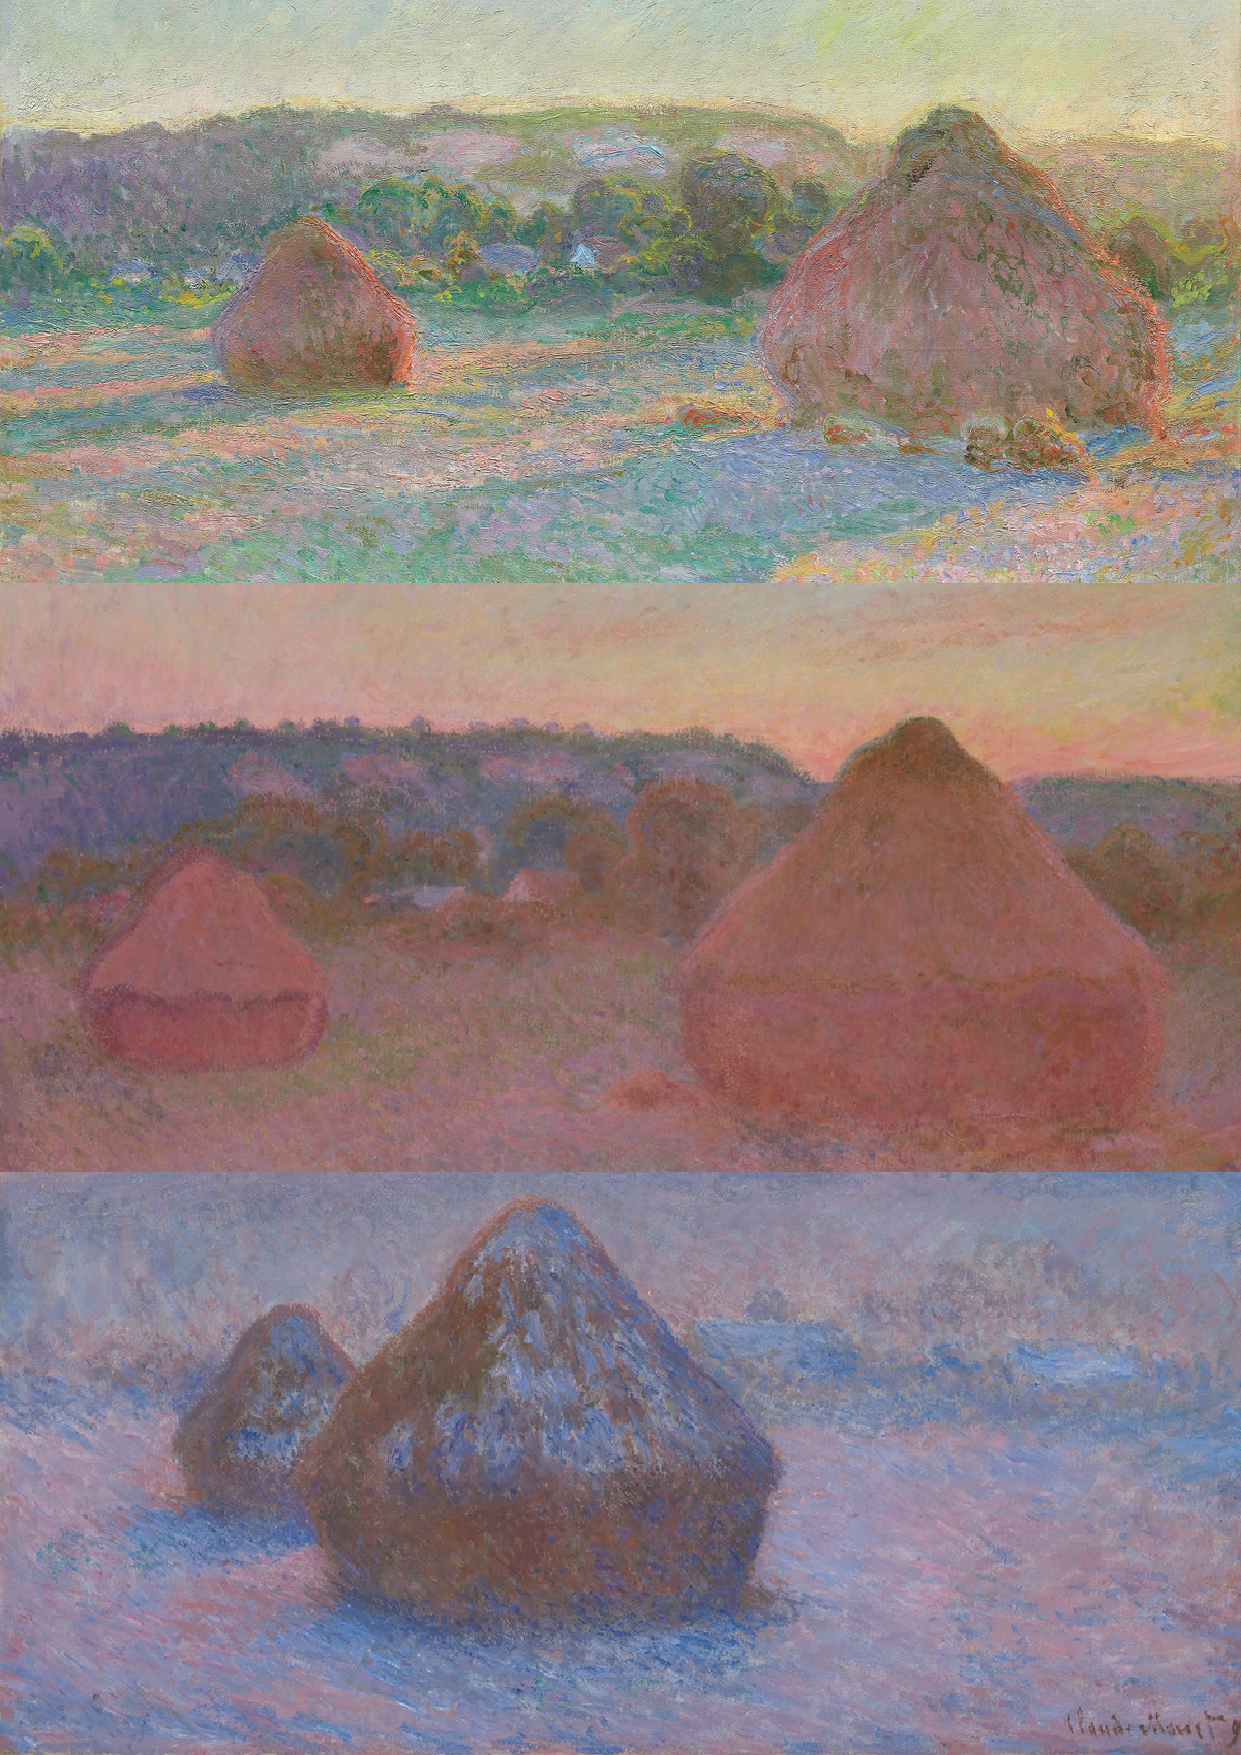
\includegraphics[width=\paperwidth]{Pictures/last.pdf}}; % Background image
\draw[anchor=north] (midpoint) node [fill=red!50!red,fill opacity=0,text opacity=1,inner xsep=1cm, inner ysep=2cm]{%
\Huge\centering\sffamily\parbox[c][][t]{\paperwidth}{%
\centering\scalefont{1.5}\vspace{15pt}%\\[15pt]
\vspace{1.3cm}
\makebox[\paperwidth][c]{{\Huge\titlefont\scalefont{1.5} \textbf{You've reached the end,}}}\\[5pt]
\makebox[\paperwidth][c]{{\Huge\titlefont\scalefont{2} \textbf{Don't Panic.}}}\\[-25pt]


\vspace{12.5cm}



% \makebox[\paperwidth][l]{{\Large\scalefont{1} \textbf{\hspace{1cm}Contributors \hfill Editors\hspace{1cm} }}}\\[-25pt]
% \makebox[\paperwidth][l]{{\Large\fontfamily{ppl}\selectfont \hspace{1 cm} David Abbe \hfill Guilherme Caumo \hspace{1cm} }}\\[-25pt]
% \makebox[\paperwidth][l]{{\Large\fontfamily{ppl}\selectfont \hspace{1cm} Minh Au \hfill Varun Muralidharan \hspace{1cm} }}\\[-25pt]
% \makebox[\paperwidth][l]{{\Large\fontfamily{ppl}\selectfont \hspace{1cm} Catherine Boisvert}\hspace{1cm}}\\[-25pt]
% \makebox[\paperwidth][l]{{\Large\fontfamily{ppl}\selectfont \hspace{1cm} Guilherme Caumo}\hspace{1cm}}\\[-25pt]
% \makebox[\paperwidth][l]{{\Large\fontfamily{ppl}\selectfont \hspace{1cm} Aditya Chugh}\hspace{1cm}}\\[-25pt]
% \makebox[\paperwidth][l]{{\Large\fontfamily{ppl}\selectfont \hspace{1cm} Félix Desroches}\hspace{1cm}}\\[-25pt]
% \makebox[\paperwidth][l]{{\Large\fontfamily{ppl}\selectfont \hspace{1cm} Daniel Jacob}}\\[-25pt]
% \makebox[\paperwidth][l]{{\Large\fontfamily{ppl}\selectfont \hspace{1cm} Varun Muralidharan}}\\[-25pt]
% \makebox[\paperwidth][l]{{\Large\fontfamily{ppl}\selectfont \hspace{1cm} Amelia Remnant}}
% 

\makebox[\paperwidth][c]{{\large\scalefont{1} {McGill Graduate Association of Physics Students \textcopyright ~2026}}}

}}; % Author name
\node[anchor=south west, inner sep=4pt,
        fill=black, fill opacity=0, text opacity=1,
        rounded corners=2pt] at (11.5cm, -1cm)
    {\small\sffamily\color{black}\textit{Stacks of Wheat} (1890-91) series by Claude Monet};
\end{tikzpicture}};
\end{tikzpicture}
\endgroup

\let\cleardoublepage\clearpage

%----------------------------------------------------------------------------------------

\end{document}
